\documentclass[15pt, a4paper]{book}

\usepackage{amsmath}    % for mathematical symbols and equations
\usepackage{amsfonts}   % for math fonts
\usepackage{amssymb}    % for extra symbols
\usepackage{graphicx}   % for including images
\usepackage{fancyhdr}   % for custom headers/footers
\usepackage{hyperref}   % for hyperlinks
\usepackage{tocbibind}  % to include the bibliography in the table of contents
\usepackage{epstopdf}   % to include .eps filesd
\usepackage{float}      % for floating figures
\usepackage{a4}         % for A4 paper size
\usepackage{fontspec}   % for custom fonts
\usepackage{xunicode}   % for unicode support
\usepackage{xltxtra}    % for XeTeX extras
\usepackage{xeCJK}      % for CJK support
\usepackage{siunitx}    % for SI units

% Title and author information
\title{A-Level Notes for Pearson Edexcel}
\author{Michael Tang}
\date{Compile Date: \today}

% Page style
\pagestyle{fancy}
\fancyhead[L]{A-Level Notes}
\fancyhead[C]{}
\setCJKmainfont[
    Path = ./fonts/,
    UprightFont = *
]{STKAITI.TTF}

\begin{document}

% Title page
\maketitle
\newpage

% Table of Contents
\tableofcontents
\newpage

% Include the chapters from each subject folder
\chapter{Math}


\chapter{Biology}

\section{Molecules, Transport, Health}
\subsection{Chemistry for Biologists}
% ===========================
%       Chapter 1A.1
%     Chemistry of Life
%   Created by Michael Tang
%        2024.12.29
% ===========================

\subsubsection{1A.1 Chemistry of Life}
\paragraph{\underline{Ionic Bonding} (离子键)}
\begin{itemize}
    \item \textbf{Definition:} Atoms transfer electrons to achieve a stable electron configuration, resulting in positively
    charged cations and negatively charged anions.
    \item \textbf{Key Properties:}
    \begin{itemize}
        \item High melting and boiling points.
        \item Solubility in polar solvents like water.
    \end{itemize}
    \item \textbf{Example:} \underline{Sodium} ($Na$ 钠) and \underline{chlorine} ($Cl$ 氯) form sodium chloride ($NaCl$ 氯).
    Sodium donates an electron to chlorine, forming a strong ionic bond.
    \begin{figure}[H]
        \centering
        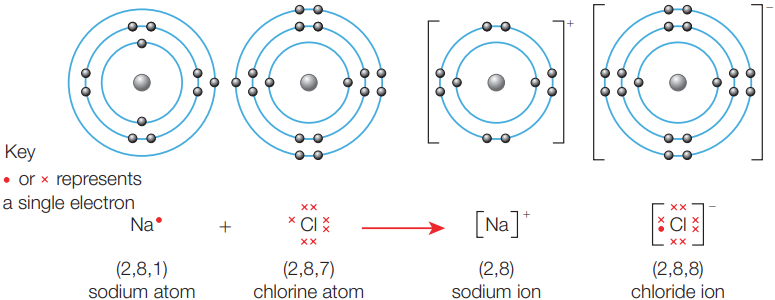
\includegraphics[scale=0.8]{Biology/1A/Images/1A-1-1.png}
        \caption{The formation of sodium chloride.}
    \end{figure}
\end{itemize}

\paragraph{\underline{Covalent Bonding} (共价键)}
\begin{itemize}
    \item \textbf{Definition:} Atoms shere electrons to achieve stability.
    \item \textbf{\underline{Polarity} (极性):} Unequal sharing of electrons leads to \underline{polar molecules} (极性分子 e.g.,
    water).
    \item \textbf{\underline{Dipoles} (偶极子):} Partial charges within the molecule, represented as $\delta^+$ (positive) and
    $\delta^-$ (negative).
    \begin{figure}[H]
        \centering
        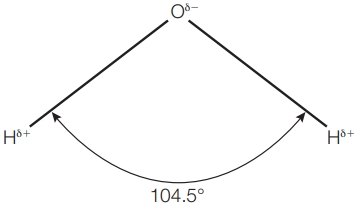
\includegraphics[scale=0.35]{Biology/1A/Images/1A-1-3.png}
        \caption{A model of a water molecule showing dipoles.}
    \end{figure}
    \item \textbf{Examples:} Formation of \underline{hydrogen} ($H_2$ 氢气) molecules and the formation of \underline{water}
    ($H_2O$ 水).
    \begin{figure}[H]
        \centering
        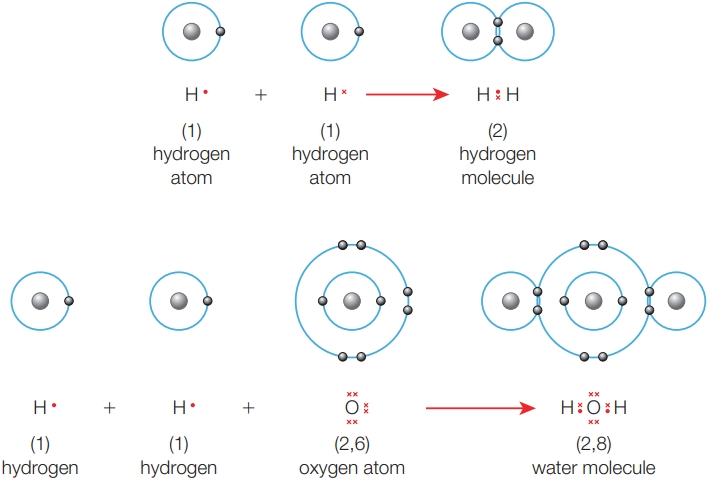
\includegraphics[scale=0.3]{Biology/1A/Images/1A-1-2.png}
        \caption{The formation of hydrogen molecules and water molecules are examples of covalent bonding.}
    \end{figure}
\end{itemize}

\paragraph{Chemistry of Water}
\begin{itemize}
    \item \textbf{Molecular Structure}
    \begin{itemize}
        \item \textbf{Polar Molecule:} Water ($H_2O$) has a bent structure with a partial charges (see figure 2.2) - oxygen is
        $\delta^-$, and hydrogen is $\delta^+$.
        \item \textbf{\underline{Hydrogen Bonding} (氢键):} Weak attractions between water molecules, providing
        \underline{cohesion} (凝聚力) and a relatively high boiling point.
        \begin{figure}[H]
            \centering
            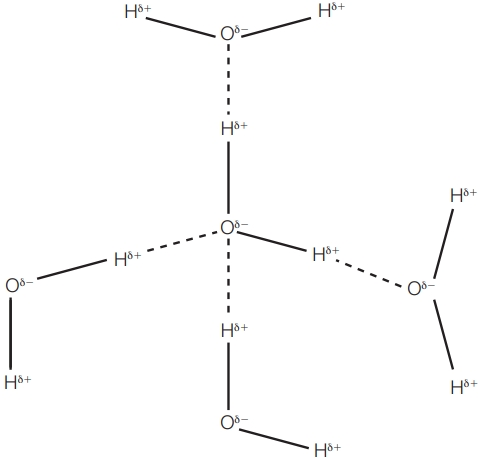
\includegraphics[scale=0.3]{Biology/1A/Images/1A-1-5.png}
            \caption{Hydrogen bonding in water molecules, based on attraction between positive and negative dipoles.}
        \end{figure}
    \end{itemize}
    \item \textbf{Unique Properties}
    \begin{itemize}
        \item \textbf{\underline{Solvent} (溶剂) Properties}
        \begin{itemize}
            \item Excellent solvent for ionic and polar \underline{substances} (物质).
            \begin{figure}[H]
                \centering
                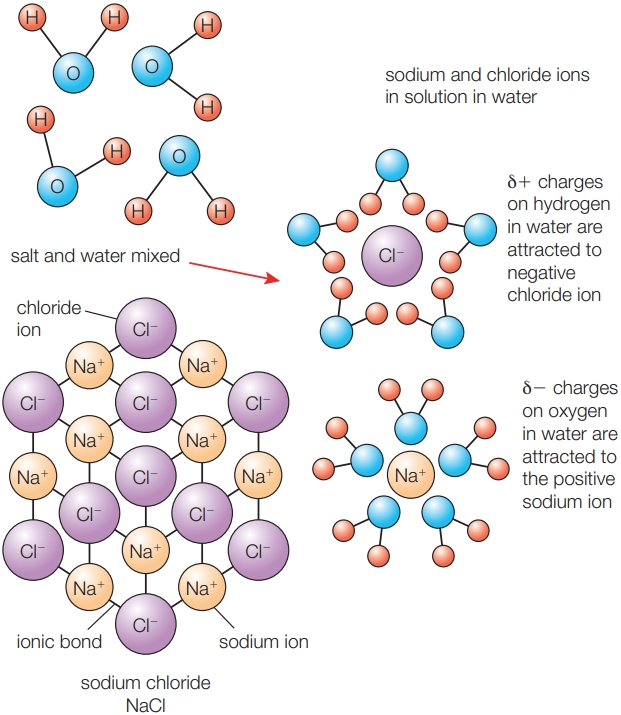
\includegraphics[scale=0.25]{Biology/1A/Images/1A-1-4.png}
                \caption{A model of sodium chloride dissolving in water as a result of the interactions between the charges on
                sodium and chloride ions and the dipoles of the water molecules.}
            \end{figure}
            \item \underline{Facilitates} (促进) \underline{biochemical} (生化) reactions in \underline{aqueous solutions} (水溶液).
        \end{itemize}
        \item \textbf{\underline{Thermal} (热) Stability}
        \begin{itemize}
            \item High specific \underline{heat capacity} \footnote{\textbf{Heat capacity: } Heat capacity refers to the amount of
            heat energy required to raise the temperature of a substance by one degree Celsius. It reflects the substance's
            ability to store \underline{thermal energy} (热能). $c$ is the symbol of heat capacity. The general formula of heat
            capacity is $c = \frac{Q}{m \left(t - t_0\right)} = \frac{Q}{m \Delta t}$. $\unit{J.kg^{-1}.K^{-1}}$ is the SI unit
            of heat capacity and $\frac{J}{(kg \cdot ^{\circ} C)}$ is the common unit.} (比热容) moderates temperature changes.
            \item Ice floats due to lower \underline{density} (密度) compared to liquid water, \underline{insulating} (隔热) the
            \underline{aquatic} (水生) life.
        \end{itemize}
        \item \textbf{\underline{Cohesion} (凝聚力) and \underline{Adhesion} (粘附力)}
        \begin{itemize}
            \item Enables water transport in plants.
            \item High surface tension due to hydrogen bonding.
        \end{itemize}
    \end{itemize}
\end{itemize}

\paragraph{Importance of Water}
\begin{itemize}
    \item \textbf{Biological Reactions:} All cellular reactions occur in an aqueous environment.
    \item \textbf{Transport Medium:} Dissolves and carries \underline{nutrients} (营养物质), gases, and \underline{waste products}
    (废物).
    \item \textbf{Habitat:} Provides a stable environment for \underline{diverse} (多样的) life forms.
    \item \textbf{Temperature Regulation:}
    \begin{itemize}
        \item \underline{Evaporation} (蒸发) cools organisms.
        \item High specific heat stability ecosystems.
    \end{itemize}
    \item \textbf{Structural Support:} \underline{Turgor pressure} \footnote{\textbf{Turgor pressure:} Turgor pressure is the
    pressure exerted by the water-filled \underline{vacuole} (液泡) against the cell wall in plant cells. It results from water
    entering the cell by \underline{osmosis} (渗透) and helps maintain the cell's \underline{rigidity} (刚性), supporting the
    plant's structure and preventing \underline{wilting} (枯萎).} (胀压) in plants depends on water.
\end{itemize}

\paragraph{Importance of \underline{Inorganic} (无机) Ions}
\begin{itemize}
    \item \textbf{Nitrate Ions ($NO_3^-$ 硝酸根离子):} Vital for DNA \footnote{\textbf{DNA (Deoxyribonucleic Acid 脱氧核糖核酸):} DNA
    is a molecule that carries the \underline{genetic instructions} (遗传信息) used in the growth, development, functioning, and
    reproduction of all living organisms. It consists of two strands forming a double \underline{helix} (螺旋), with each
    \underline{strand} (股) made up of \underline{nucleotide bases} (核苷酸碱基) (adenine 腺嘌呤, thymine 胸腺嘧啶, cytosine 胞嘧啶,
    and guanine 鸟嘌呤). These \underline{bases pair} (碱基对) specifically (A-T, C-G) and encode the instructions for
    \underline{synthesizing} (合成) proteins, which determine an organism's \underline{traits} (特征).} and \underline{protein
    synthesis} (蛋白质合成) in plants. (see sections 1A.5, 2B.3, and chapter 5A).
    \item \textbf{Phosphate Ions ($PO_4^{3-}$ 磷酸根离子):} Essential for ATP \footnote{\textbf{ATP (Adenosine Triphosphate
    腺嘌呤核苷三磷酸):} ATP is a molecule that acts as the primary energy carrier in cells. It consists of an \underline{adenosine
    molecule} (腺苷分子) bonded to three \underline{phosphate} (磷酸盐) groups. When ATP is broken down into ADP (adenosine
    diphosphate 二磷酸腺苷/核苷酸) and a phosphate group, energy is released to fuel cellular processes such as muscle contraction,
    active transport, and chemical synthesis.}, DNA \footnotemark[3], and RNA \footnote{\textbf{RNA (Ribonucleic Acid 核糖核酸):}
    RNA is a \underline{single-stranded nucleic acid} (单链核酸) that plays a crucial role in protein synthesis and gene
    expression. It is composed of \underline{ribose sugar} (核糖/单糖), phosphate groups, and four \underline{nitrogenous bases}
    (含氮碱基): adenine (A 腺嘌呤), uracil (U 尿嘧啶), cytosine (C 胞嘧啶), and guanine (G 鸟嘌呤). Unlike DNA, RNA contains uracil
    instead of thymine. Types of RNA include: mRNA \footnotemark[6] (messager RNA 信使核糖核酸), tRNA \footnotemark[7] (transfer
    RNA 转运核糖核酸), and rRNA \footnotemark[8] (ribosomal RNA 核糖体).} (see section 2B.3 and chapter 5A).
    \footnotetext[6]{\textbf{mRNA:} mRNA is a type of RNA that carries the genetic information from DNA in the cell nucleus to
    the \underline{ribosome} (核糖体), where it is used as a template for protein synthesis. It is transcribed from DNA and
    contains \underline{codons} \footnotemark[9] (密码子) that specify the \underline{amino acids} (氨基酸) to be incorporated
    into the protein.}
    \footnotetext[7]{\textbf{tRNA:} tRNA is a type of RNA that helps decode the genetic instructions in mRNA during protein
    synthesis. It carries specific amino acids to the ribosome, where it pairs its \underline{anticodon} \footnotemark[10]
    (反密码子) with the complementary codon on the mRNA sequence. This ensures that amino acids are added in the correct sequence
    to form a protein.}
    \footnotetext[8]{\textbf{rRNA:} rRNA is a type of RNA that is a key structural and functional component of ribosomes, the
    \underline{molecular machines} \footnotemark[11] (分子机器) that synthesize proteins. rRNA helps align mRNA and tRNA during
    protein synthesis and catalyzes the formation of \underline{peptide bonds} (肽键) between amino acids, facilitating the
    assembly of proteins.}
    \footnotetext[9]{\textbf{Codon:} A codon is a sequence of three nucleotide bases in mRNA that corresponds to a specific
    amino acid or a stop signal during protein synthesis. For example, the \underline{codon AUG} \footnotemark[12] (起始密码子)
    codes for the amino acid \underline{methionine} (蛋氨酸) and also serves as the start signal for translation.}
    \footnotetext[10]{\textbf{Anticodon:} An anticodon is a sequence of three nucleotide bases on a tRNA molecule that is
    complementary to a codon on the mRNA strand. During protein synthesis, the anticodon pairs with its corresponding codon,
    ensuring that the correct amino acid is added to the growing polypeptide chain.}
    \footnotetext[11]{\textbf{Molecular machines:} Molecular machines are complex biomolecules or assemblies of molecules that
    perform specific tasks within a cell, often converting energy into mechanical work. Examples include ribosomes for protein
    synthesis, ATP synthase for energy production, and \underline{motor proteins} \footnotemark[13] (马达蛋白) like
    \underline{kinesin} (驱动蛋白) for \underline{intracellular transport} (细胞内运输).}
    \footnotetext[12]{\textbf{Codon AUG:} The codon AUG serves two critical roles in protein synthesis: start codon, it signals
    the beginning of translation, indicating where the ribosome should start assembling the protein; and amino acid, AUG codes
    for the amino acid methionine (Met), which is often the first amino acid in newly synthesized proteins. This dual function
    makes AUG essential in the initiation of protein synthesis.}
    \footnotetext[13]{\textbf{Motor proteins:} Motor proteins are specialized molecular machines that convert chemical energy
    from ATP into mechanical work to perform cellular movements. They play key roles in intracellular transport, cell division,
    and structural support. Examples include: \underline{kinesin} (驱动蛋白), \underline{dynein} (动力蛋白), and \underline{myosin}
    (肌球蛋白).}
    \item\textbf{Chloride Ions ($Cl^-$ 氯离子):} Needed in all living organisms to make AT and ADP as well as DNA and RNA (see
    chapters 7C and 8A).
    \item \textbf{Hydrogencarbonate Ions ($HCO_3^-$ 碳酸氢根离子):} Needed in nerve impulses, sweating, and many
    \underline{secretory systems} (分泌系统) in animals (see section 1B.2).
    \item \textbf{Sodium Ions ($Na^+$ 钠离子):} Critical in nerve impulses and secretory functions (see chapter 8A).
    \item \textbf{Magnesium Ions ($Mg^{2+}$ 镁离子):} Needed for production of \underline{chorophyll} (叶绿素) in plants (see
    chapter 5A).
    \item \textbf{Hydrogen Ions ($H^+$ 氢离子):} Needed in cellular \underline{respiration} (呼吸) and \underline{photosynthesis}
    (光合作用), and in numerous pumps and systems as well as pH balance (see section 2A.4 and chapters 5A and 7A).
    \item \textbf{Calcium Ions ($Ca^{2+}$ 钙离子):} Needed for the formation of \underline{calcium pectate} (果胶酸钙) for middle
    \underline{lamella} (中膜) between two cell walls in plants, and for bone formation and muscle contraction in animals (see
    section 4A.1 and chapters 7B and 7C).
\end{itemize}

% ===========================
%       Chapter 1A.2
%      Carbohydrates:
%   Mono- and Disaccharides
%   Created by Michael Tang
%        2024.12.30
% ===========================

\subsubsection{1A.2 Carbohydrates: Monosaccharides and Disaccharides}
\paragraph{What are Organic Compounds?}
\begin{itemize}
    \item \textbf{Definition:} Organic compounds are molecules containing carbon atoms bonded to hydrogen and other elements, such
    as oxygen, nitrogen, and phosphorus. In some carbon compounds small molecules (\underline{monomers} 单体) bond with many
    other similar units to make a very large molecule called a \underline{polymer} (聚合物). The ability of carbon to combine and
    make \underline{macromolecules} (大分子) is the basis of all biological molecules and provides the great variety and
    complexity found in living things.
    \begin{figure}[H]
        \centering
        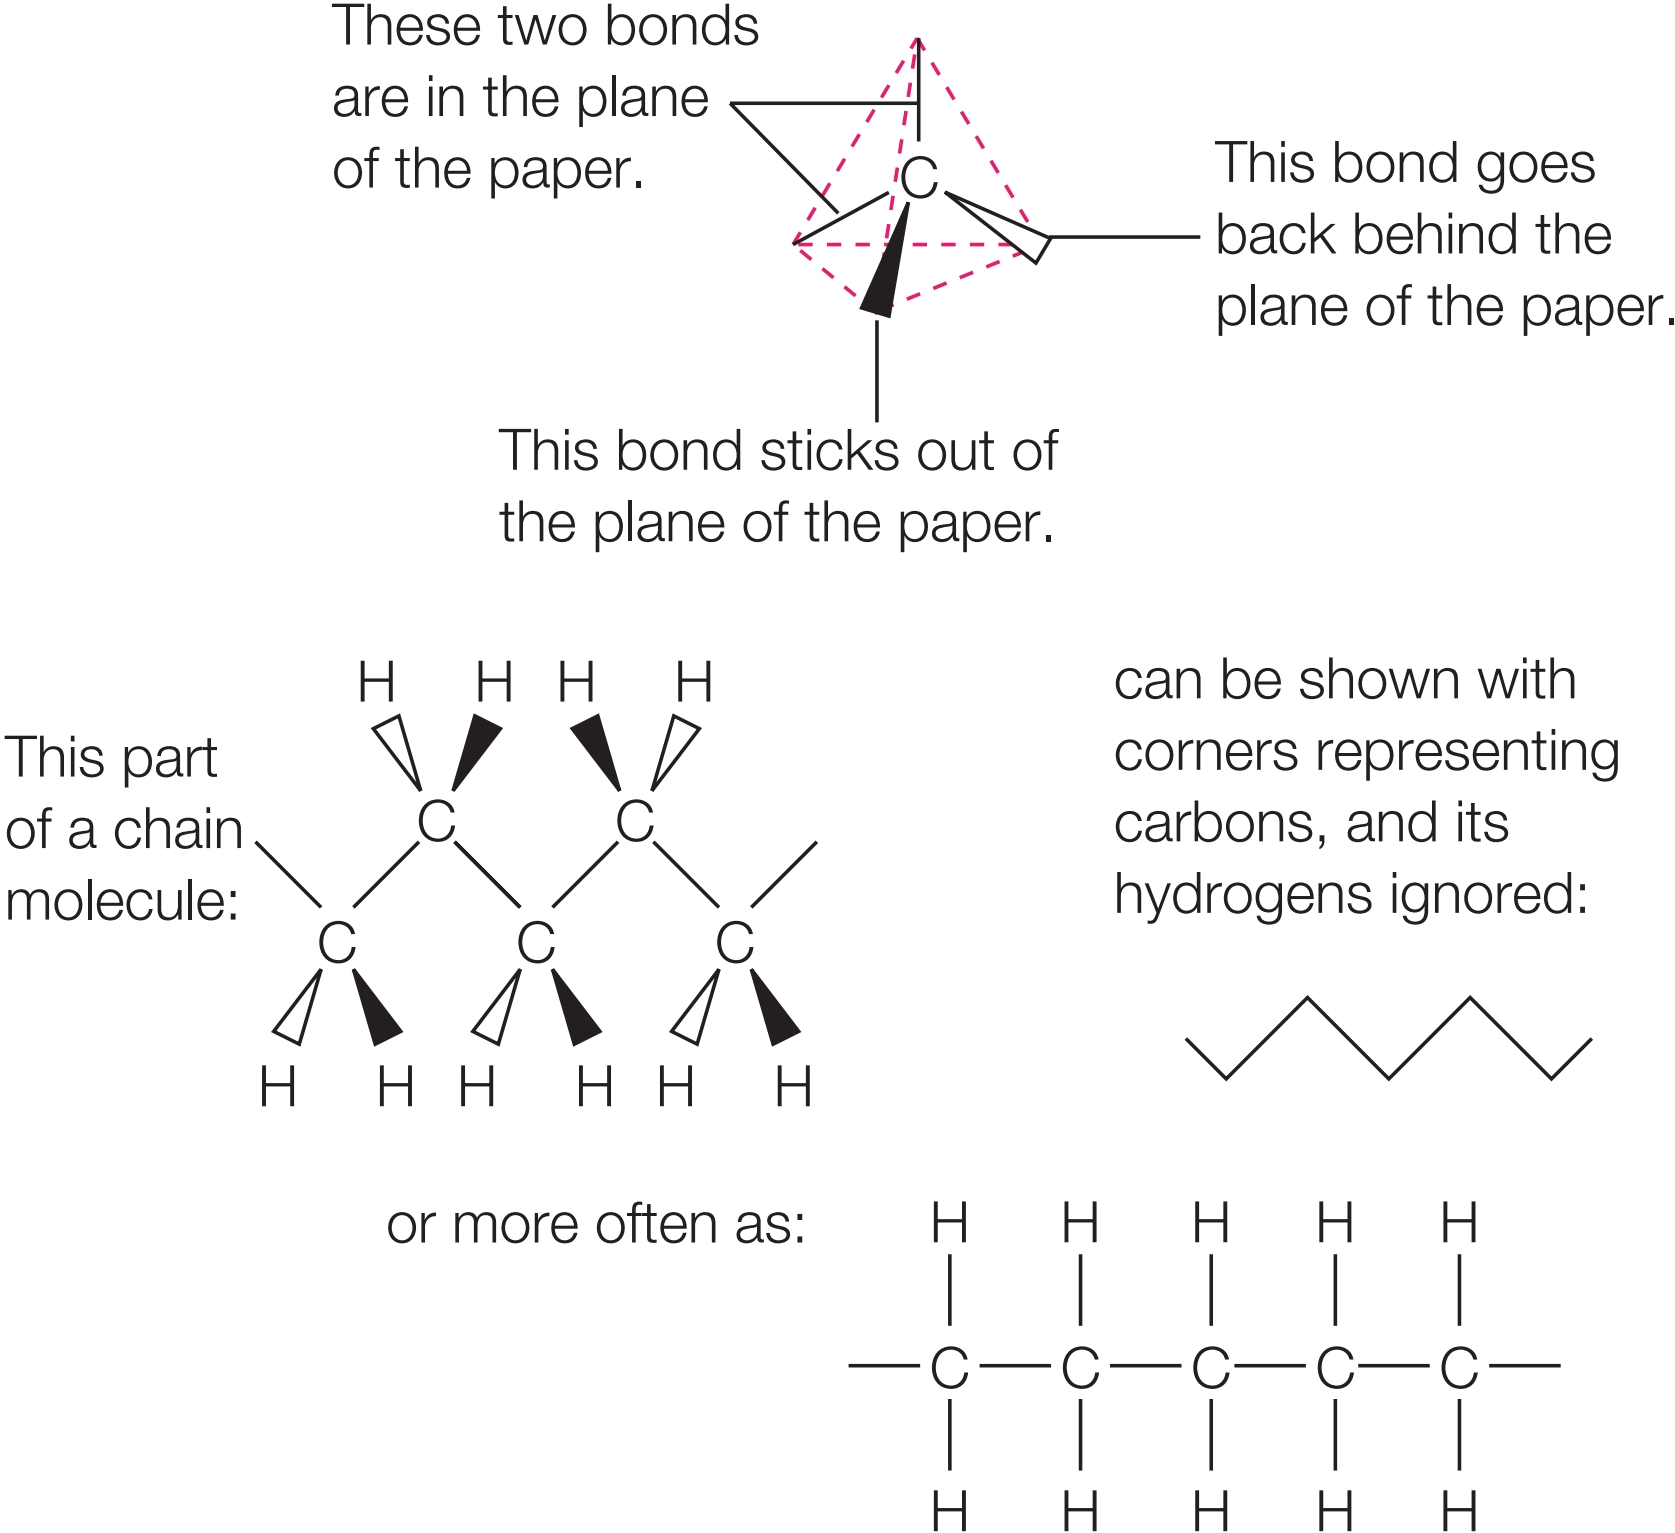
\includegraphics[scale=0.18]{Biology/1A/Images/1A-2-1.png}
        \caption{The bonds in a carbon atom have a complicated 3D shape. This is difficult to represent, so in most molecular
        diagrams we use one of several different ways to draw them.}
    \end{figure}
    \item \textbf{Key Features:}
    \begin{itemize}
        \item Carbon atoms form stable covalent bonds, allowing complex structures.
        \item Organic compounds include \underline{carbohydrates} (碳水化合物), \underline{lipids} (脂质), \underline{proteins}
        (蛋白质), and \underline{nucleic acids} (核酸).
    \end{itemize}
\end{itemize}

\paragraph{Carbohydrates}
Carbohydrates are essential organic molecules, primarily serving as energy sources and structural components. They are composed
of carbon (\ce{C} 碳), hydrogen (\ce{H} 氢), and oxygen (\ce{O} 氧), typically in a 1:2:1 ratio - \ce{(CH2O)_n}.

\paragraph{\underline{Monosaccharides} (单糖): The Simplest Sugars}
\begin{itemize}
    \item \textbf{Key Characteristics:}
    \begin{itemize}
        \item Simplest form of carbohydrates.
        \item General formula: \ce{(CH2O)_n}, where $n$ is the number of carbon. Although $n$ can be any number, but it
        is usually low (3-7).
        \item Examples:
        \begin{itemize}
            \item \textbf{Triose (3-Carbon 三糖, $n=3$):} \ce{C3H6O3}. E.g., \underline{glyceraldehyde} (甘油醛), involved in
            \underline{glycolysis} (糖酵解).
            \item \textbf{Pentose (5-Carbon 五糖, $n=5$):} \ce{C5H10O5}. E.g., \underline{ribose} (核糖) and
            \underline{deoxyribose} (脱氧核糖).
            \begin{figure}[H]
                \centering
                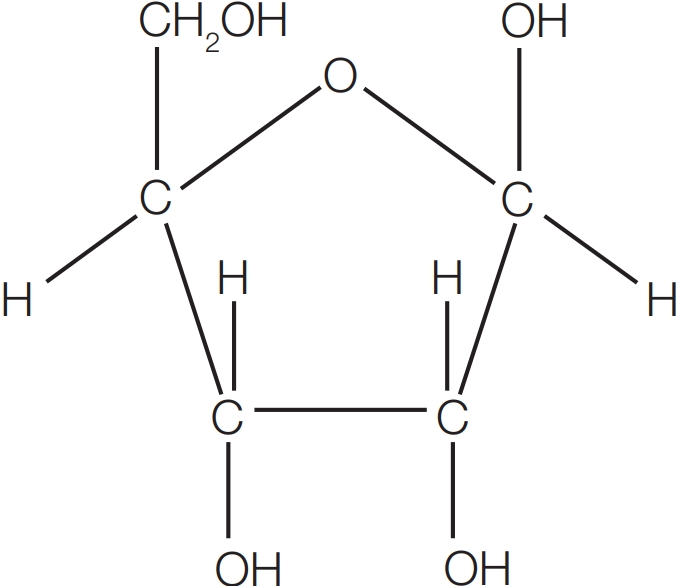
\includegraphics[scale=0.25]{Biology/1A/Images/1A-2-2.png}
                \caption{Pentose sugars such as ribose have 5 carbon atoms.}
            \end{figure}
            \item \textbf{Hexose (6-Carbon 六糖 , $n=6$):} \ce{C6H12O6}. E.g., glucose (energy source 葡萄糖), fructose (fruit
            sugar 果糖), galactose (milk sugar 半乳糖).
        \end{itemize}
        \item Structure of Glucose
        \begin{itemize}
            \item Gulcose has two \underline{isomers} (different forms 同分异构体): $\alpha$-glucose and $\beta$-glucose. The two
            isomers have different arrangements of the atoms on the side chains of the molecule.
            \item \textbf{Alpha($\alpha$) glucose:} \underline{Hydroxyl} (\ce{-OH} 羟基) group on carbon 1 is below the plane.
            \item \textbf{Beta($\beta$) glucose:} Hydroxyl group on carbon 1 is above the plane.
        \end{itemize}
        \begin{figure}[H]
            \centering
            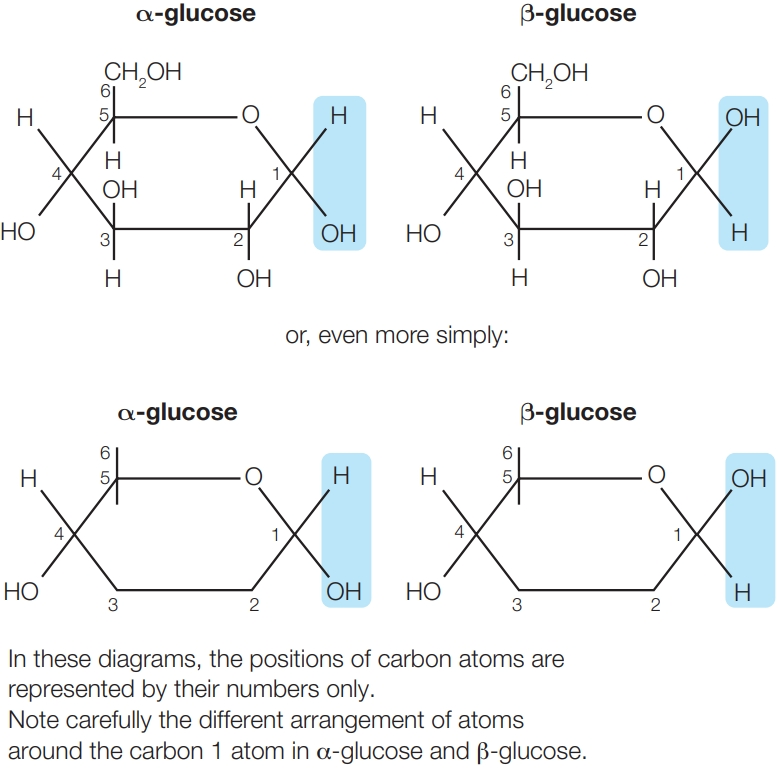
\includegraphics[scale=0.28]{Biology/1A/Images/1A-2-3.png}
            \caption{Hexose sugars have a ring structure. The arrangement of the atoms on the side chains can make a significant
            difference to the way in which the molecule can be used by the body. The carbon atoms are numbered in order to
            identify the different arrangements.}
        \end{figure}
    \end{itemize}
\end{itemize}

\paragraph{\underline{Disaccharides} (二糖): The Double Sugars}
\begin{itemize}
    \item \textbf{Formation:}
    \begin{itemize}
        \item \textbf{\underline{Condensation Reaction} (缩合反应):} Two monosaccharides join, forming a \underline{glycosidic
        bond} (糖苷键) and releasing a water molecule (\ce{H2O}).
        \begin{figure}[H]
            \centering
            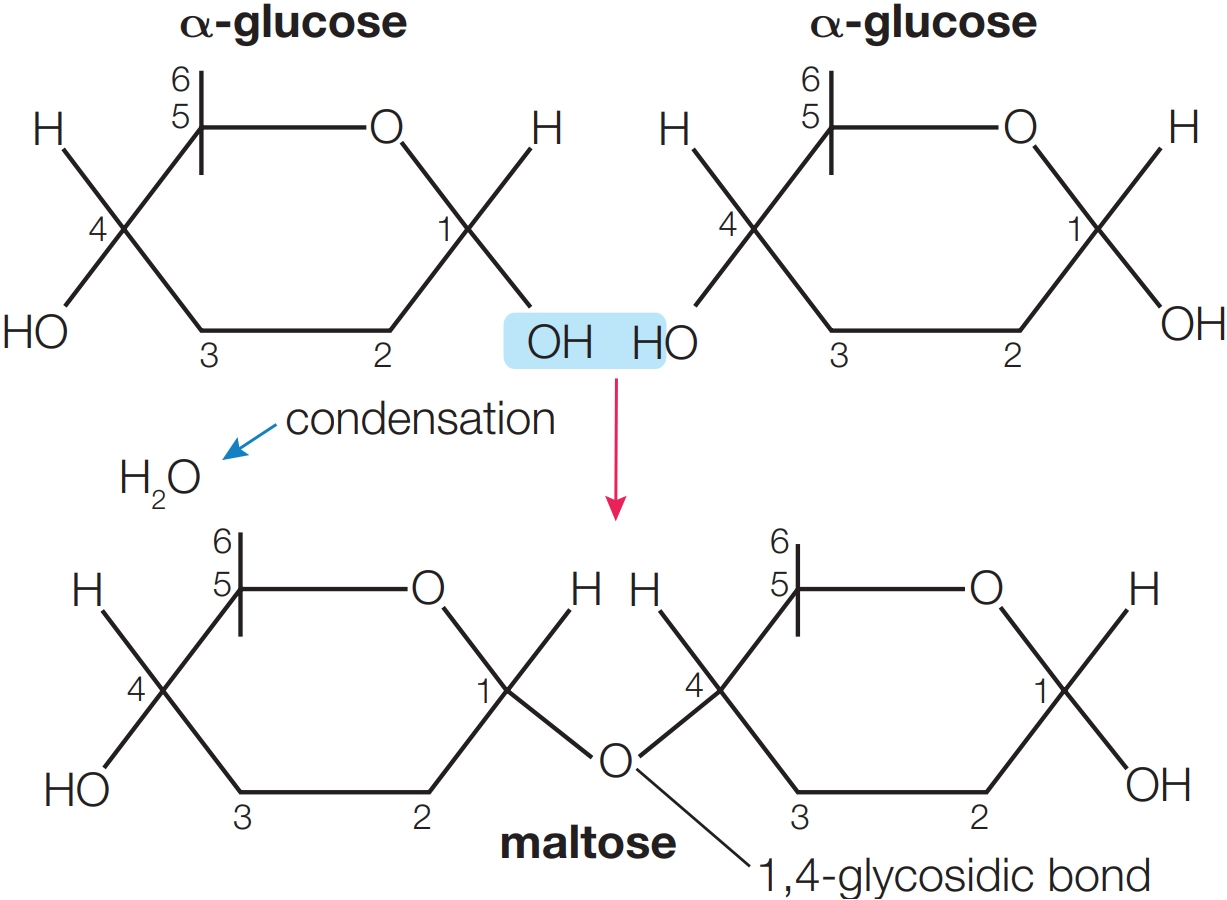
\includegraphics[scale=0.18]{Biology/1A/Images/1A-2-4.png}
            \caption{The formation of a glycosidic bond. The condensation reaction between two monosaccharides results in a
            disaccharide and a molecule of water.}
        \end{figure}
        \item \textbf{Examples:}
        \begin{itemize}
            \item \textbf{\underline{Sucrose} (蔗糖):} Glucose + Fructose. Stored in plants such as \underline{sugar cane} (甘蔗).
            \item \textbf{\underline{Lactose} (乳糖):} Glucose + Galactose. Milk sugar - this is the main carbohydrate found in
            milk.
            \item \textbf{\underline{Maltose} (麦芽糖):} Glucose + Glucose. \underline{Malt} (麦芽) sugar - found in
            \underline{germinating} (发芽) seed such as \underline{barley} (大麦).
        \end{itemize}
    \end{itemize}
    \item \textbf{Breakdown - \underline{Hydrolysis Reaction} (水解反应):} Glycosidic bonds are broken with the
    \underline{addition} (添加) of water, \underline{yielding} (产生) two monosaccharides.
\end{itemize}

\paragraph{Testing for Sugars - \underline{Benedict's Test} (本尼迪克特试验)}
\begin{itemize}
    \item \textbf{Principle:} Benedict's test is a \underline{qualitative test} \footnote{\textbf{Qualitative Test:} A qualitative
    test determines the \underline{presence} (存在) or \underline{absence} (不存在) of a specific substance in a sample, without
    providing \underline{precise} (精确的) numerical data about its \underline{concentration} (浓度) or \underline{quantity} (数量)
    \begin{itemize}
        \item \textbf{Key Features:}
        \begin{itemize}
            \item \textbf{Purpose:} Identify whether a substance is present.
            \item \textbf{Outcome:} Results are typically \underline{descriptive} (描述性的 - e.g., color change, precipitation
            沉淀, or effervescence 泡沫) rather than \underline{quantitative} (定量性的).
            \item \textbf{Examples in Biology and Chemistry:} Benedict's test for reducing sugars (color change from blue to
            brick-red), iodine test for starch (color change from yellow-brown to blue-black), and \underline{biuret test}
            (缩二脲试验) for proteins (color change from blue to purple).
        \end{itemize}
        \item \textbf{Limitations:}
        \begin{itemize}
            \item Does not measure the exact amount of a substance.
            \item \underline{Subjective interpretation} (主观解释)  of results (e.g., intensity of color change 颜色变化的程度).
        \end{itemize}
    \end{itemize}} (定性实验) used to detect the presence of \underline{reducing sugars} (还原糖). These sugars can reduce copper
    (II) ions (\ce{Cu^2+}) to copper (I) ions (\ce{Cu^+}) due to the presence of a free \underline{aldehyde} (\ce{R-CHO} \footnote{In
    organic chemistry \ce{R} is a \underline{shorthand symbol} (缩写符号) used to represent a generic \underline{alkyl group} (烷基)
    or \underline{side chain} (侧链) attached to a \underline{functional group} \footnotemark[9] (官能团). It is a
    \underline{placeholder} (占位符) for any group of carbon and hydrogen atoms (and sometimes other atoms) in a molecule.
    \begin{itemize}
        \item \textbf{Explanation of \ce{R} in \ce{R-CHO}:}
        \begin{itemize}
            \item \ce{R}: Represents a \underline{hydrocarbon} (烃/碳氢化合物) chain or group, such as:
            \begin{itemize}
                \item \underline{Methyl group} (甲基): \ce{CH3-}
                \item \underline{Ethyl group} (乙基): \ce{CH3CH2-}
                \item \underline{Cycloalkyl group} (环烷基): \ce{C6H11}
                \item Longer or branched alkyl chains: \ce{C_nH_{2n+1}}
            \end{itemize}
            \item \ce{CHO}: Represents the \underline{aldehyde functional group} (醛官能团), where a carbon atom is
            \underline{double-bonded} (双键) to an oxygen atom (\ce{C=O}) and \underline{single-bonded} (单键) to a hydrogen atom
            (\ce{-H}).
        \end{itemize}
        \item \textbf{Purpose of \ce{R}:}
        \begin{itemize}
            \item[1.] \textbf{Generic Representation:} It simplifies chemical structures when the specific nature of the alkyl
            group is not important for the discussion.
            \item[2.] \textbf{Flexibility:} Allows focus on the functional group (\ce{CHO}) rather than the details of the alkyl
            chain.
        \end{itemize}
        \item \textbf{Examples:} Methanal (Formaldehyde 甲醛): \ce{H-CHO}, where \ce{R=H}.
    \end{itemize}} 醛) or
    \underline{ketone} (\ce{R-CO-R}$'$ \footnote{\ce{R-CO-R}$'$ can also write as $>$\ce{C=O}. In organic chemistry, the symbol $>$\ce{C=O} is used
    to describe the structure of a \underline{carbonyl group} (羰基), emphasizing that the carbon atom in the carbonyl group is
    bonded not only to an oxygen atom but also to two other \underline{groups} (基团). The $>$ symbol indicates that the carbonyl
    carbon is an \underline{internal carbon} (内部碳), connected to two other groups or chains (rather than being a terminal
    carbon).} 酮) group.
    \footnotetext[9]{\textbf{Functional group:} A functional group is a specific group of atoms within a molecule that
    determines the chemical properties and reactions of that molecule. It is the reactive part of the molecule, often defining
    its behavior in biological or chemical processes. Functional groups are crucial in organic chemistry because they dictate how
    molecules interact and bond with others.}
    \item \textbf{Reducing sugars:} Reducing sugars include monosaccharides like glucose, fructose, and galactose, and
    disaccharides except sucrose. They have the ability to donate electrons to other molecules due to their reactive carbonyl
    group.
    \item \textbf{Reagents in Benedict's Test:} Benedict's Solution contains:
    \begin{itemize}
        \item \textbf{Copper (II) Sulfate (\ce{CuSO4}):} Source of (\ce{Cu^2+}) ions.
        \item \textbf{Sodium Citrate (\ce{C6H5Na3O7}):} Stablizes the copper (II) ions in the solution.
        \item \textbf{Sodium Carbonate (\ce{Na2CO3}):} Provides an alkaline environment.
    \end{itemize}
    \item \textbf{Chemical Reaction:}
    \begin{itemize}
        \item[1.] In an alkaline medium, the carbonyl group of the reducing sugar reacts with the copper (II) ions.
        \item[2.] Reduction Process:
        \begin{itemize}
            \item \ce{Cu^2+} (blue) is reduced to \ce{Cu^+} (red/orange precipitate of copper (I) oxide, \ce{Cu2O}).
            \item Reaction:
            \begin{equation}
                \ce{R-CHO + 2Cu^2+ + 5OH^- -> R-COOH + Cu2O + 2H2O}
            \end{equation}
            Where \ce{R-CHO} represents the reducing sugar.
        \end{itemize} 
    \end{itemize}
    \item \textbf{Procedure:}
    \begin{itemize}
        \item[1.] Mix the sample with Benedict's solution.
        \item[2.] Heat the mixture in a boiling water bath for about 2-5 minutes.
        \item[3.] Observe the color change and precipitate formation.
    \end{itemize}
    \item \textbf{Observation and Results:}
    \begin{table}[h!]
        \centering
        \begin{tabular}{|l|l|}
        \hline
        \textbf{Color Change}          & \textbf{Reducing Sugar Concentration} \\ \hline
        Blue (no change)               & No reducing sugar present             \\ \hline
        Green                          & Low concentration                     \\ \hline
        Yellow                         & Moderate concentration                \\ \hline
        Brick-red precipitate          & High concentration                    \\ \hline
        \end{tabular}
        \caption{Color changes observed in Benedict's test for reducing sugars.}
        \label{tab:reducing_sugars}
    \end{table}
    \begin{figure}[H]
        \centering
        \includegraphics[scale=1]{Biology/1A/Images/1A-2-5.bmp}
        \caption{Benedict's test for reducing sugars.}
    \end{figure}
    \item \textbf{Limitations:} Non-reducing sugars like sucrose do not react directly unless hydrolyzed.
\end{itemize}
% ===========================
%       Chapter 1A.3
%      Carbohydrates:
%     Polysaccharides
%   Created by Michael Tang
%        2024.12.30
% ===========================

\subsubsection{1A.3 Carbohydrates: \underline{Polysaccharides} (多糖)}
\paragraph{Carbohydrates and Energy}
Carbohydrates are a primary source of energy in biological systems, particularly glucose, which is a key monosaccharide used in
cellular respiration.
\begin{itemize}
    \item \textbf{Key Points}
    \begin{itemize}
        \item \textbf{Energy Production:} Glucose (\ce{C6H12O6}) is broken down through cellular respiration to produce ATP
        (adenosine triphosphate), which powers cellular activities.
        \item \textbf{End Products:} The breakdown of glucose result in:
        \begin{itemize}
            \item Carbon dioxide (\ce{CO2})
            \item Water (\ce{H2O})
            \item Large amounts of ATP
        \end{itemize}
        \item \textbf{Glucose Utilization:}
        \begin{itemize}
            \item \textbf{Monosaccharides} such as glucose are rapidly absorbed and used for immediate energy needs.
            \item \textbf{Disaccharides} like sucrose and lactose are broken into monosaccharides for energy production.
            \item \textbf{Polysaccharides} are complex carbohydrates made up of many monosaccharide units joined by glycosidic
            bonds. Note that molecules with between 3 and 10 sugar units are known as \underline{\textbf{oligosaccharides}}
            (低聚糖), while molecules containing 11 or more monosaccharides are known as true polysaccharides.
            \begin{figure}[H]
                \centering
                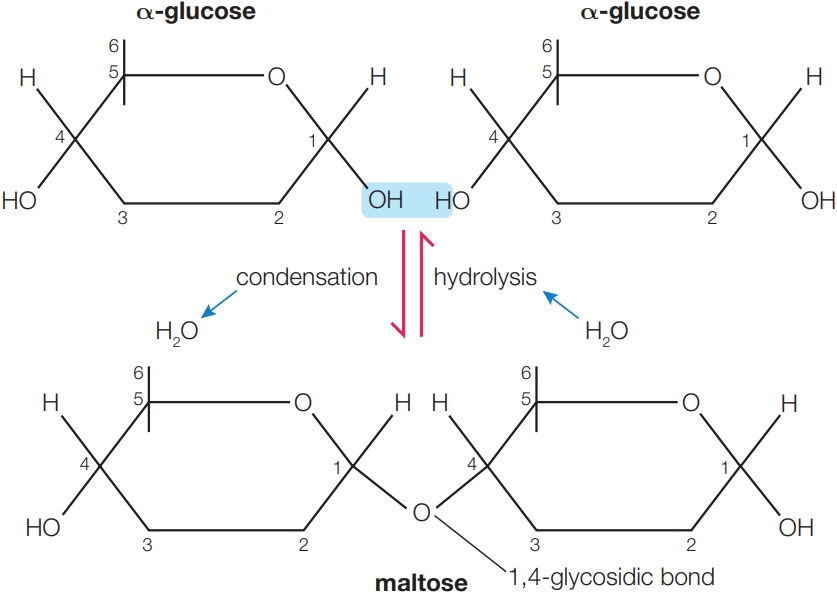
\includegraphics[scale=0.3]{Biology/1A/Images/1A-3-1.png}
                \caption{Glycosidic bonds are made by condensation reactions and broken down by hydrolysis.}
            \end{figure}
            \item \textbf{Exam Hint:} Avoid stating that energy is "created". Instead, describe how chemical energy from glucose
            is transferred to ATP molecules.
        \end{itemize}
    \end{itemize}
    \item \textbf{Properties of Polysaccharides}
    \begin{itemize}
        \item[1.] \textbf{Compact Structure:}
        \begin{itemize}
            \item Takes up little space within cells.
            \item Ideal for storage purposes.
        \end{itemize}
        \item[2.] \textbf{Insolubility:}
        \begin{itemize}
            \item Reduces \underline{osmotic effects} \footnote{\textbf{Osmotic effects:} Osmotic effects refer to the movement
            of water across a \underline{semipermeable membrane} \footnotemark[10] (半透膜) due to differences in solute
            concentration.} (渗透效应) in cells.
            \footnotetext[10]{\textbf{Semipermeable membrane:} It is a membrane that allows certain molecules to pass through
            while blocking others. It permits solvent molecules (such as water) to pass but prevents solute molecules from doing
            so. This property makes semipermeable membranes highly useful in various applications, such as
            \underline{desalination} (海水淡化), where water and salt in seawater are separated using a semipermeable membrane.}
            \item Does not affect water potential.
        \end{itemize} 
        \item[3.] \textbf{Chemical Inactivity:} Does not interfere with cellular reactions.
    \end{itemize}
    \item \textbf{Starch (Plant Energy Store)}
    \begin{itemize}
        \item Composed of $\alpha$-glucose units.
        \item Two main components:
        \begin{itemize}
            \item \textbf{\underline{Amylose} (直链淀粉):} Long, unbranched chains of $\alpha$-glucose units. Forms a compact
            spiral sturcture due to 1,4-glycosidic bonds.
            \item \textbf{\underline{Amylopectin} (支链淀粉):} Branched chains of $\alpha$-glucose units. Contains 1,4- and 1,6-
            glycosidic bonds, allowing rapid glucose release.
        \end{itemize}
        \begin{figure}[H]
            \centering
            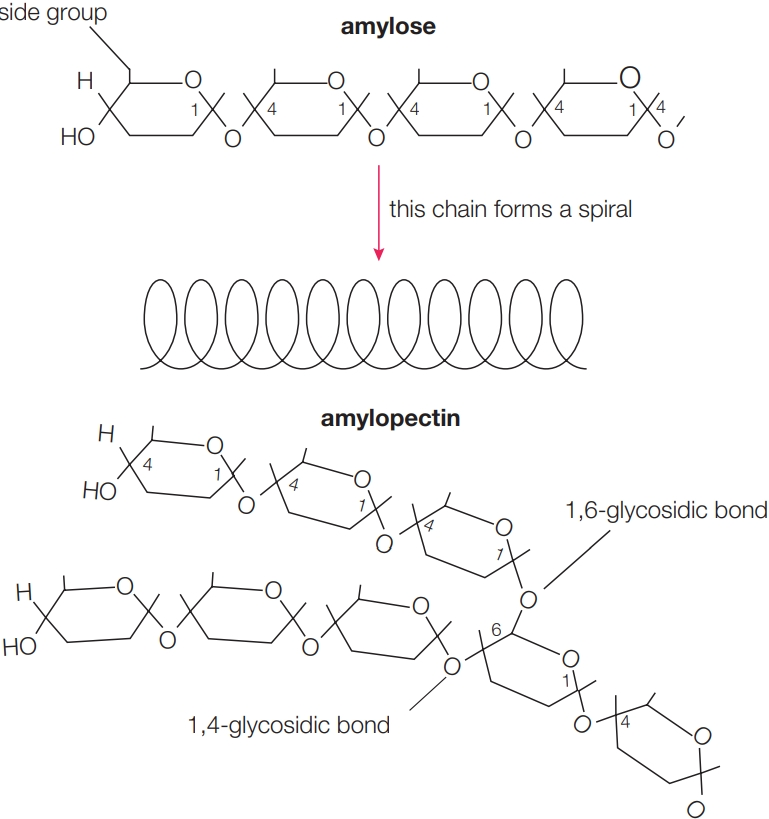
\includegraphics[scale=0.35]{Biology/1A/Images/1A-3-2.png}
            \caption{Amylose and amylopectin — a small difference in the position of the glycosidic bonds in the molecule makes
            a big difference to the properties of the compounds.}
        \end{figure}
        \item \textbf{Function:}
        \begin{itemize}
            \item Efficient energy storage in plants.
            \item Rapid glucose availability during high metabolic demands.
        \end{itemize}
        \item \textbf{Testing for Starch} If you add a few drops of reddish-brown iodine solution to a sample containing starch
        (whether it is a solid sample or a sample in solution), the iodine solution will turn blue-black.
        \begin{figure}[H]
            \centering
            \includegraphics[scale=1]{Biology/1A/Images/1A-3-5.bmp}
            \caption{The iodine test for starch.}
        \end{figure}
    \end{itemize}
    \item \textbf{Glycogen (Animal Energy Store)}
    \begin{itemize}
        \item Similar to amylopectin but more extensively branched.
        \item \textbf{Structure:}
        \begin{itemize}
            \item Contains many 1,6-glycosidic bonds, leading to multiple branches.
            \item Compact and can be rapidly hydrolyzed for energy.
        \end{itemize}
        \begin{figure}[H]
            \centering
            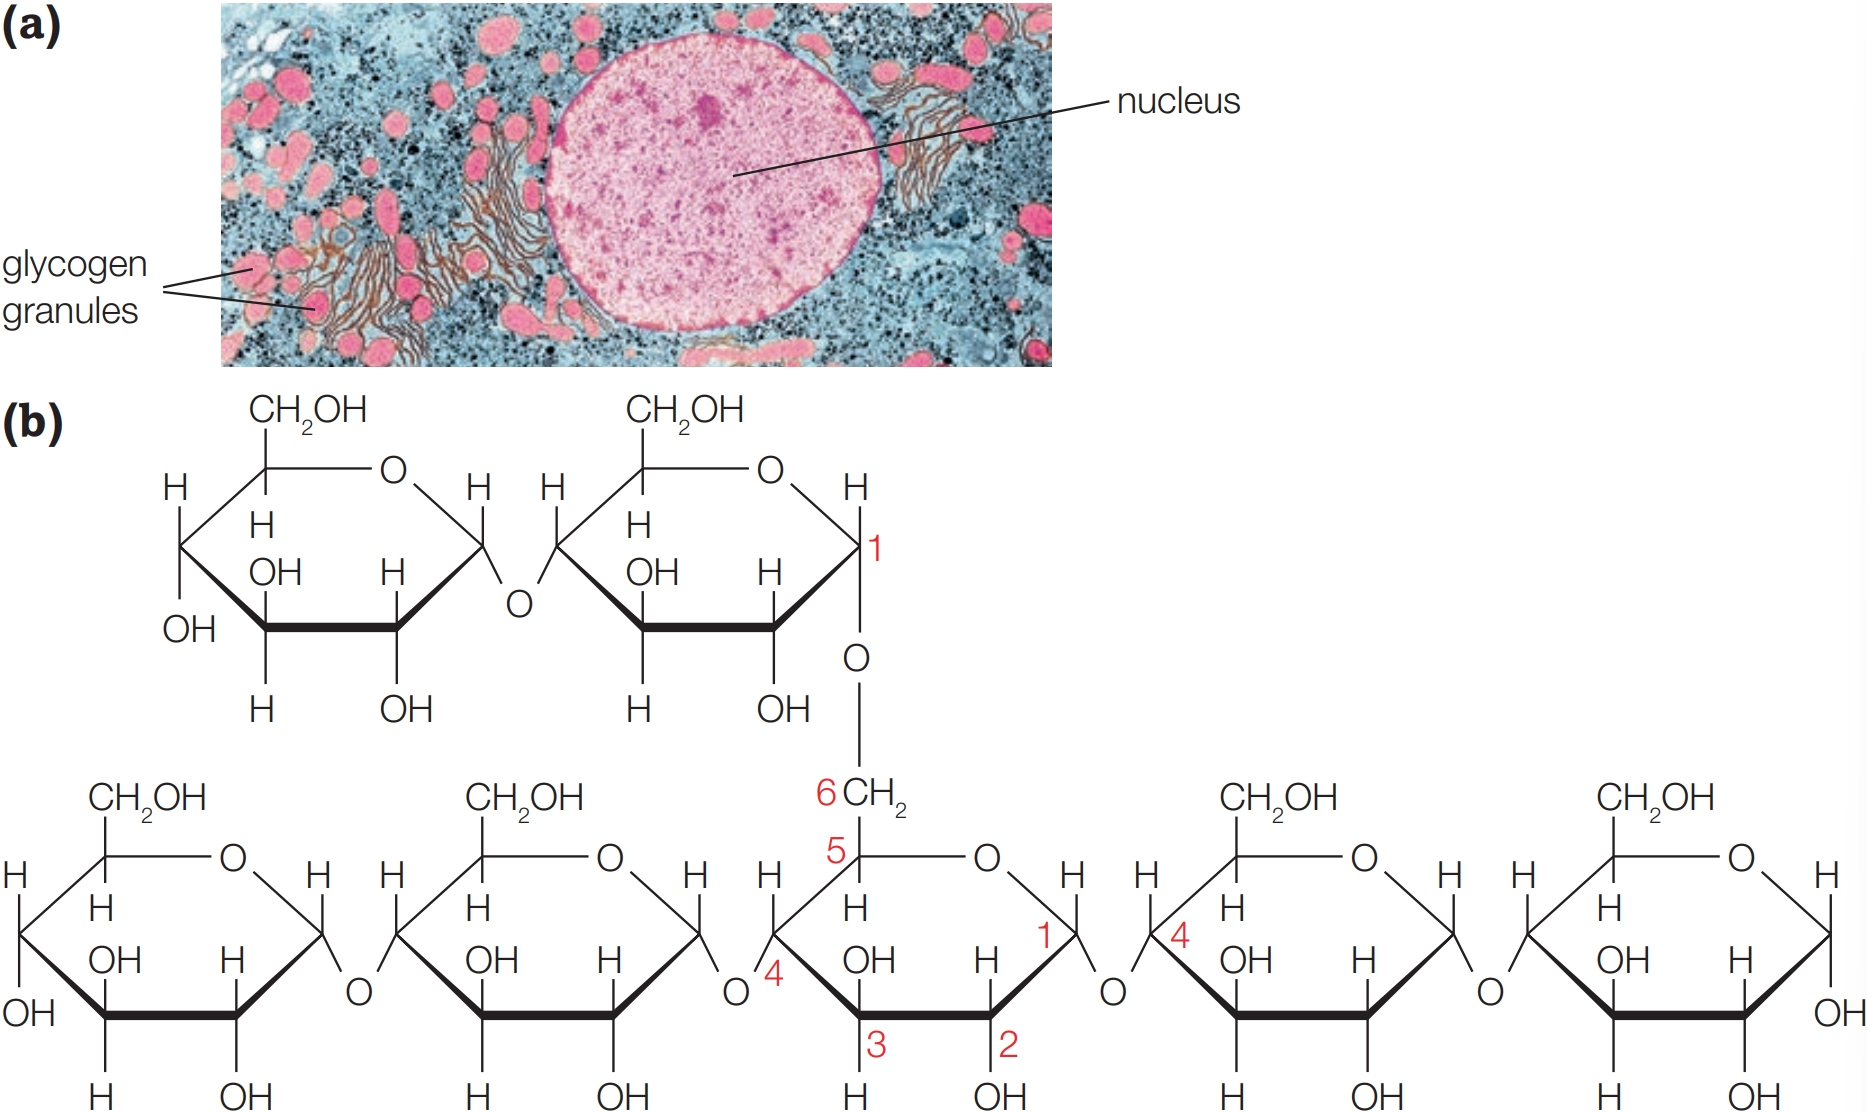
\includegraphics[scale=0.15]{Biology/1A/Images/1A-3-3.png}
            \caption{In \textbf{(a)} you can see liver cells full of small glycogen \underline{granules} (微粒), \underline{stained}
            (染色) pink in this \underline{micrograph} (显微照片). If your blood glucose levels are low, this glycogen store in
            your liver can be broken down to provide the glucose you need for cellular respiration. In \textbf{(b)} you can see the
            structure of glycogen with 1,4 and 1,6-glycosidic bonds.}
        \end{figure}
        \item \textbf{Function:}
        \begin{itemize}
            \item Found in the liver and muscle cells.
            \item Acts as a quick energy source for animal during high activity.
        \end{itemize}
        \begin{figure}[H]
            \centering
            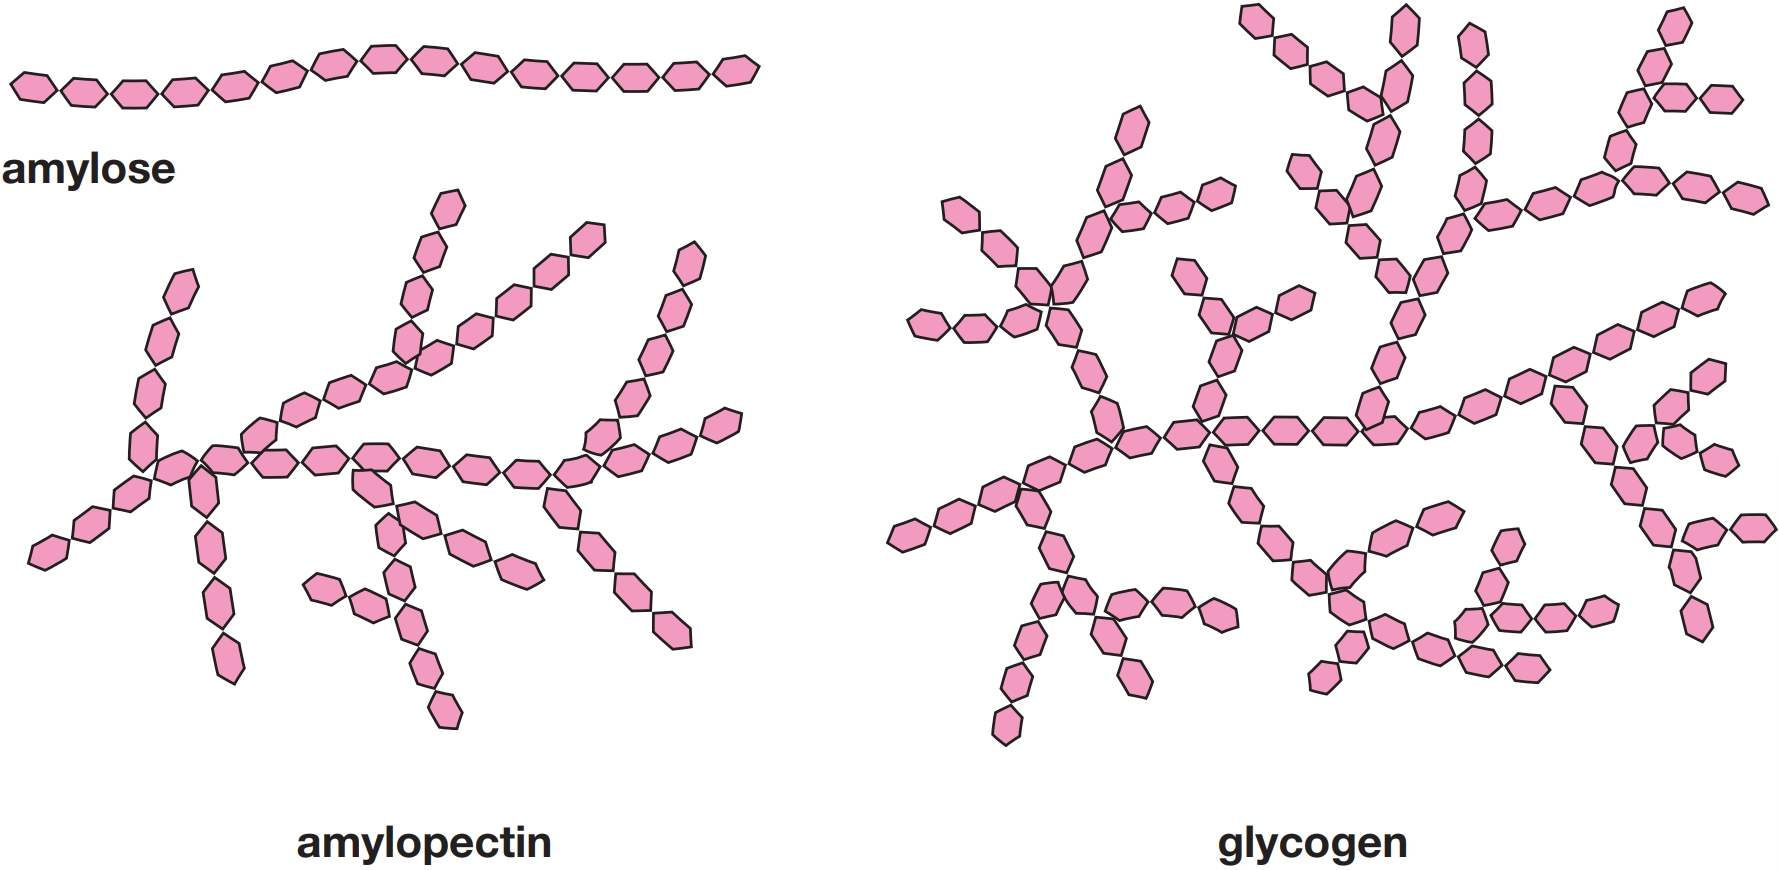
\includegraphics[scale=0.15]{Biology/1A/Images/1A-3-4.png}
            \caption{You can clearly see the many side branches which allow glycogen to be broken down so quickly when you
            compare amylose, amylopectin and glycogen.}
        \end{figure}
    \end{itemize}
\end{itemize}

% ===========================
%       Chapter 1A.4
%          Lipids
%   Created by Michael Tang
%        2024.12.30
% ===========================

\subsubsection{1A.4 \underline{Lipids} (脂类)}
\paragraph{Fats and Oils} Fats and oils are essential lipids with significant biological roles.
\begin{itemize}
    \item \textbf{Definition:} Lipids include fats and oil. Fats are solid at room temperature, while oils are liquid at room
    temperature.
    \item \textbf{Composition:}
    \begin{itemize}
        \item Made of \underline{glycerol} ($C_3H_8O_3$ 甘油) and fatty acids ($C_nH_{2n+1}COOH$ 脂肪酸).
        \begin{figure}[H]
            \centering
            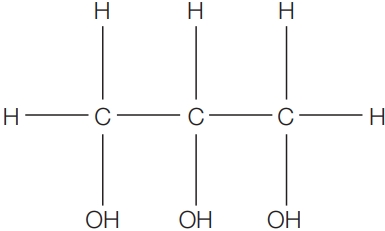
\includegraphics[scale=0.28]{Biology/1A/Images/1A-4-1.png}
            \caption{Displayed formula of glycerol (propane-1,2,3-triol).}
        \end{figure}
        \item Contain carbon ($C$), hydrogen ($H$), and small amount of oxygen ($O$) atoms.
    \end{itemize}
    \item \textbf{Sources:}
    \begin{itemize}
        \item \textbf{Fats:} \underline{Predominantly} (大多数情况下) from animal sources (e.g., butter, lard 猪油).
        \item \textbf{Oils:} Predominantly from plant sourcrs (e.g., olive oil, sunflower oil).
    \end{itemize}
    \item \textbf{Energy Content:}
    \begin{itemize}
        \item Store about three times as much energy as the same mass of carbohydrates.
        \item Act as long-term energy storage, especially in seeds and \underline{adipose tissue} (皮下脂肪组织).
    \end{itemize}
\end{itemize}

\paragraph{Fatty Acids} Fatty acids are hydrocarbon chains with a \underline{carboxyl group} ($-COOH$ 羧基) at one end.
\begin{itemize}
    \item \textbf{Types:}
    \begin{itemize}
        \item[1.] \textbf{\underline{Saturated Fatty Acids} (饱和脂肪酸):} Only single bonds between carbon atoms (e.g., stearic
        acid 硬脂酸).
        \begin{figure}[H]
            \centering
            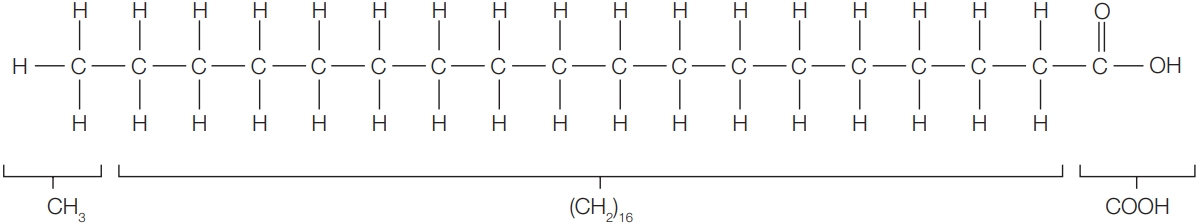
\includegraphics[scale=0.28]{Biology/1A/Images/1A-4-2.png}
            \caption{Displayed formula of stearic acid, a saturated fatty acid found in both plant and animal fats.}
        \end{figure}
        \item[2.] \textbf{\underline{Unsaturated Fatty Acids} (不饱和脂肪酸):}
        \begin{itemize}
            \item \textbf{\underline{Monounsaturated Fatty Acids} (单不饱和脂肪酸):} One double bond between carbon atoms.
            \item \textbf{\underline{Polyunsaturated Fatty Acids} (多不饱和脂肪酸):} Multiple carbon-carbon double bonds
            (e.g., linoleic acid 亚油酸).
        \end{itemize}
        \begin{figure}[H]
            \centering
            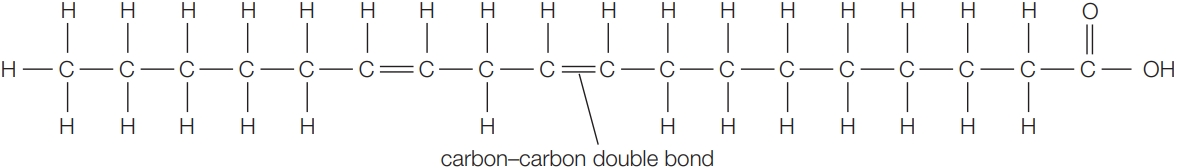
\includegraphics[scale=0.28]{Biology/1A/Images/1A-4-3.png}
            \caption{Displayed formula of linoleic acid, a polyunsaturated fatty acid.}
        \end{figure}
    \end{itemize}
    \item \textbf{Properties:}
    \begin{itemize}
        \item Saturated fats are more likely to be solid at room temperature.
        \item Unsaturated fats are usually liquid and healthier in the diet.
    \end{itemize}
\end{itemize}

\paragraph{Forming Ester Bonds} Ester bonds are formed in the synthesis of \underline{triglycerides} \footnote{Note that a
word with a prefix mono- usually means one, di- means two, tri- means three, and poly- means many.} (甘油三酯) through a
condensation reaction.
\begin{itemize}
    \item \textbf{Process:}
    \begin{itemize}
        \item[1.] \textbf{Reactants:}
        \begin{itemize}
            \item Glycerol provides hydroxyl groups ($-OH$).
            \item Fatty acids provide carboxyl groups ($-COOH$).
        \end{itemize}
        \item[2.] \textbf{Reaction:} A molecule of water ($H_2O$) is removed for each \underline{ester bond} \footnote{An ester
        bond is a covalent bond formed between the hydroxyl group ($-OH$) of glycerol and the carboxyl group ($-COOH$) of a fatty
        acid. This bond is a key structural feature of lipids, particularly triglycerides.} (酯键) formed.
        \item[3.] \textbf{Product:} One molecule of glycerol reacts with three fatty acids to form a triglyceride.
    \end{itemize}
    \item \textbf{Chemical Representation:}
    $$\text{Glycerol} + 3\text{Fatty Acids} \rightarrow \text{Triglyceride} + 3H_2O$$
    \item \textbf{Hydrolysis:} Ester bonds in triglycerides can be broken down by adding water, releasing glycerol and fatty
    acids.
    \begin{figure}[H]
        \centering
        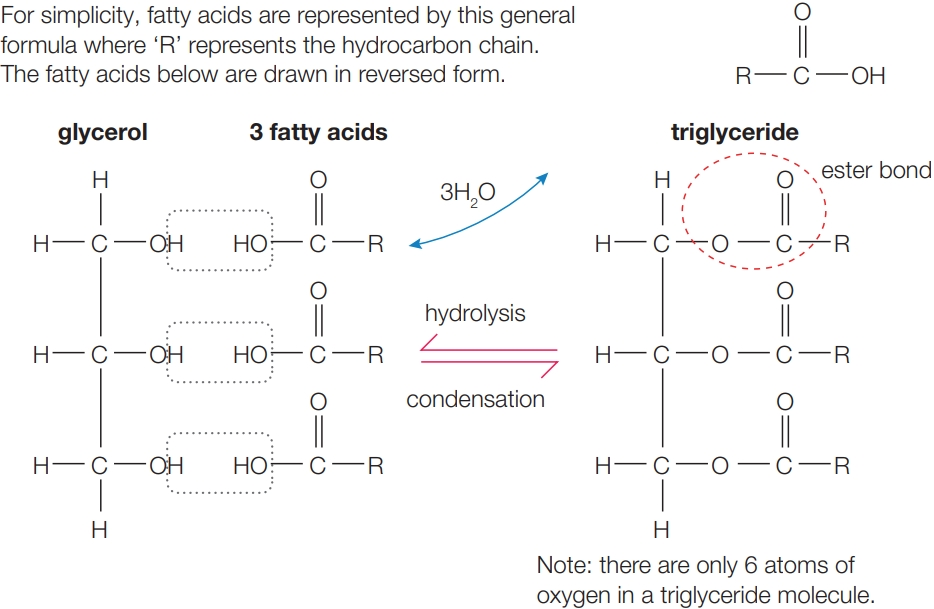
\includegraphics[scale=0.35]{Biology/1A/Images/1A-4-4.png}
        \caption{The formation of ester bonds.}
    \end{figure}
\end{itemize}
\subsection{Mammalian Transport Systems}
% ===============================
%          Chapter 1B.1
%  The Principles of Circulation
%     Created by Michael Tang
%           2025.01.01
% ===============================

\subsubsection{1B.1 The Principles of Circulation}
\paragraph{Need for Transport in Organisms}
\begin{itemize}
    \item \textbf{\underline{Diffusion} (扩散):} The movement of substances from a region of high concentration to low
    concentration. Works efficiently only in small organisms where the surface area to volume ratio (sa$:$vol) is large.
    \item \textbf{Limitations of Diffusion:} As organisms grow larger, the sa$:$vol ratio decreases, and diffusion becomes
    insufficient to meet the metabolic demands of all cells.
\end{itemize}

\paragraph{Transport in Small Organisms}
\begin{itemize}
    \item Small organisms (e.g., amoeba 阿米巴原虫/变形虫, marine larvae 海洋幼虫) rely on diffusion for transport due to:
    \begin{itemize}
        \item[1.] Short diffusion distances.
        \item[2.] Large sa$:$vol ratio (e.g., jellyfish larvae 水母幼虫)
        \item[3.] Low metabolic demands.
    \end{itemize}
    \item Surface area to volume ratio (sa$:$vol): Larger organisms have smaller sa$:$vol ratios, making diffusion less efficient.
\end{itemize}

\paragraph{Transport in Multicellular Organisms}
Larger organisms require specialized transport systems due to:
\begin{itemize}
    \item[1.] Increased metabolic demands (e.g., oxygen, nutrients, waste removal).
    \item[2.] Removal of waste products (e.g., carbon dioxide, urea 尿素).
    \item[3.] Greater distance between external environment and innermost cells.
\end{itemize}

\paragraph{Key Features of Mass Transport Systems}
\begin{itemize}
    \item[1.] \textbf{Exchange surfaces:} Efficient transport of materials in and out (e.g., gases, nutrients, waste).
    \item[2.] \textbf{Transport vessels:} Tubes to carry substances (e.g., blood vessels 血管, xylem 木质部).
    \item[3.] \textbf{Mechanisms for movement:} Pumping (e.g., heart 心脏) or maintaining concentration gradients.
    \item[4.] \textbf{Transport medium:} Fluid to carry substances (e.g., blood 血液, sap 树液).
    \item[5.] \textbf{Adaptations:} To meet the specific needs of the organism (e.g., gills 鳃, lungs 肺).
\end{itemize}

\paragraph{Circulatory Systems}
\begin{itemize}
    \item[1.] \textbf{Open Circulatory System:} Found in insects, \underline{mollusks} 软体动物, and some
    \underline{invertebrates} 无脊椎动物. Blood flows freely in the body cavity (hemocoel 血腔) and directly.
    \item[2.] \textbf{Closed Circulatory System:} Found in \underline{vertebrates} (脊椎动物) and some invertebrates. Blood is
    enclosed in blood vessels (e.g., arteries 动脉, veins 静脉, capillaries 毛细血管) and pumped by a heart.
\end{itemize}

\paragraph{Types of Circulatory Systems}
\begin{itemize}
    \item[1.] \textbf{Single Circulation:}
    \begin{itemize}
        \item Blood passes through the heart once per cycle.
        \item Heart $\rightarrow$ Gills $\rightarrow$ Body $\rightarrow$ Heart.
        \item Advantages: Simple and sufficient for lower metabolic demands.
        \begin{figure}[H]
            \centering
            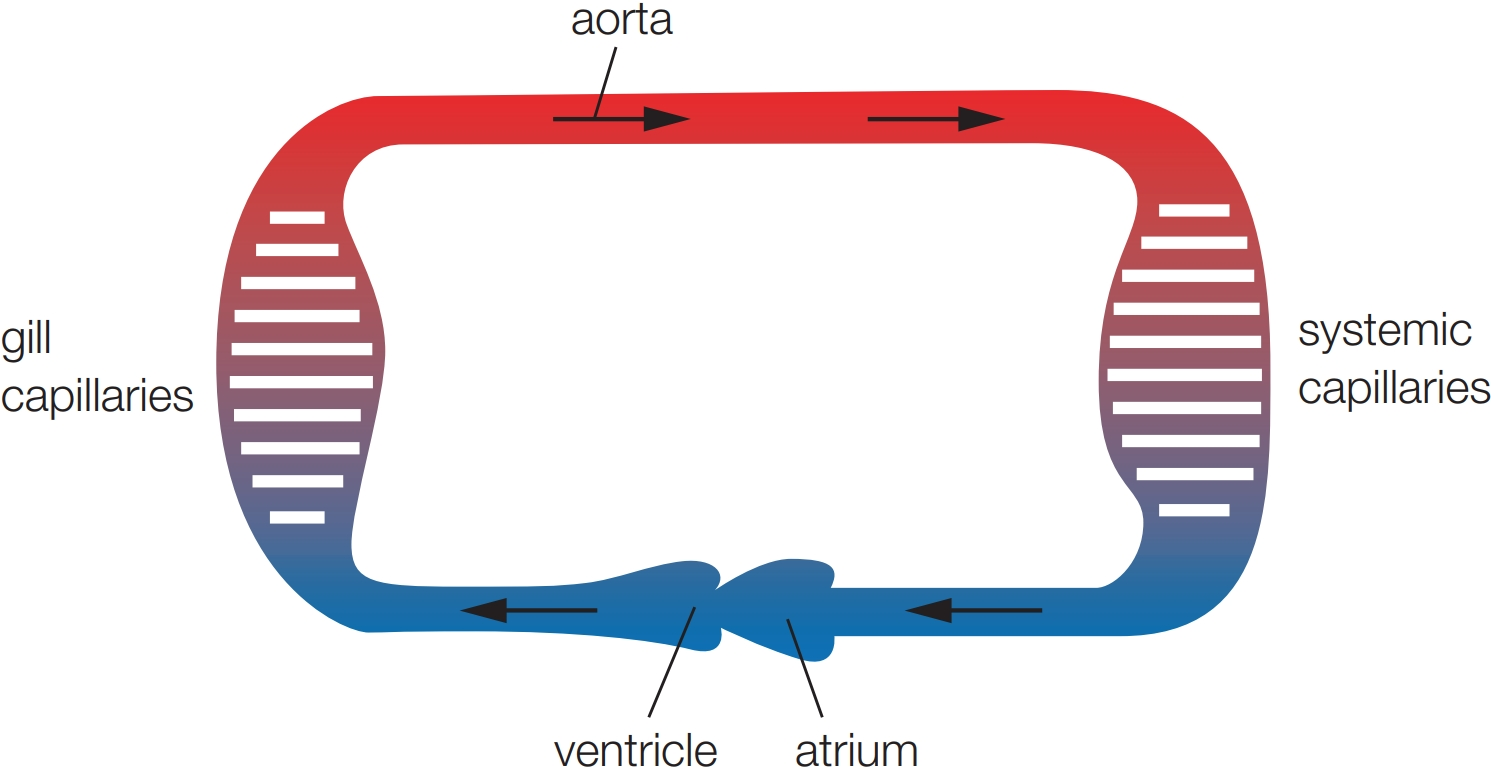
\includegraphics[scale=0.15]{Biology/1B/Images/1B-1-1.png}
            \caption{The single circulation of a fish.}
        \end{figure}
    \end{itemize}
    \item[2.] \textbf{Double Circulation:}
    \begin{itemize}
        \item Blood passes through the heart twice per cycle.
        \begin{itemize}
            \item[a)] \textbf{Pulmonary Circulation:} Heart $\rightarrow$ Lungs $\rightarrow$ Heart.
            \item[b)] \textbf{Systemic Circulation:} Heart $\rightarrow$ Body $\rightarrow$ Heart.
        \end{itemize}
        \begin{figure}[H]
            \centering
            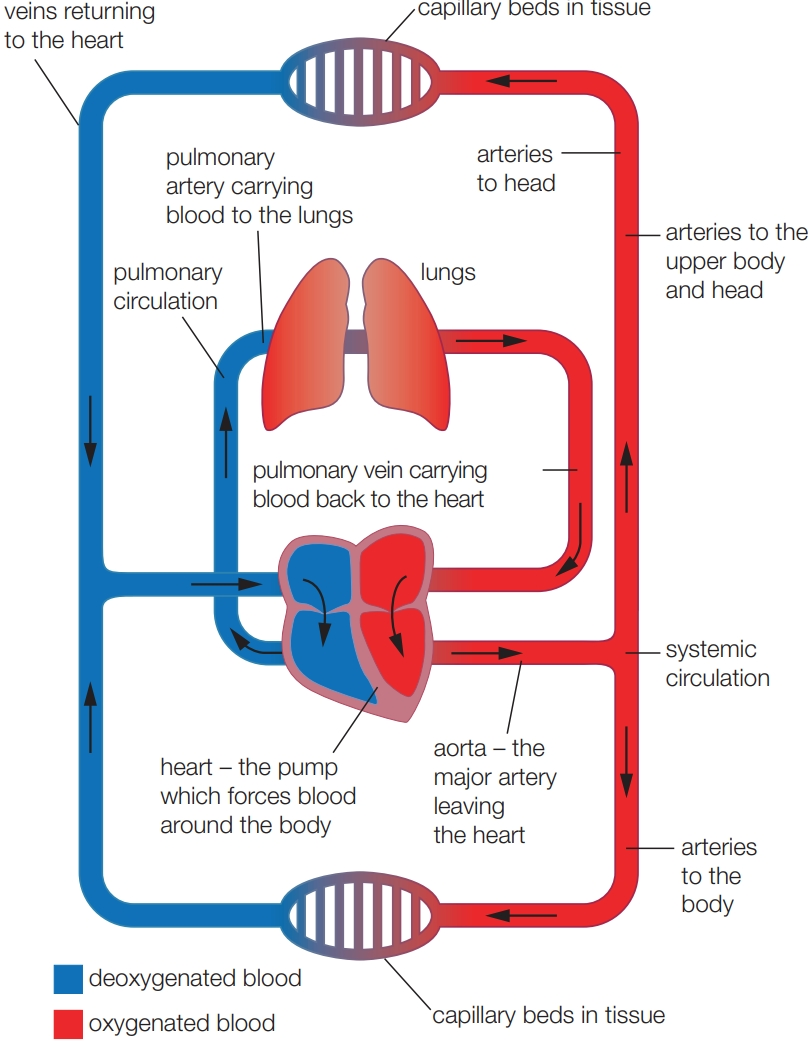
\includegraphics[scale=0.25]{Biology/1B/Images/1B-1-2.png}
            \caption{A double circulation sends blood at high pressure, carrying lots of oxygen, to the active cells of the body.
            Take note: this is a schematic diagram. In a real double circulation, all of the blood vessels enter and leave from
            the top of the heart.}
        \end{figure}
        \item Advantages:
        \begin{itemize}
            \item Maintain high blood pressure in systemic circulation.
            \item Efficient oxygen delivery to active tissues.
        \end{itemize}
    \end{itemize}
\end{itemize}
% ===============================
%          Chapter 1B.2
%     The Roles of the Blood
%     Created by Michael Tang
%           2025.01.01
% ===============================

\subsubsection{1B.2 The Roles of the Blood}
\paragraph{The \underline{Cardiovascular System} (心血管系统)}
\begin{itemize}
    \item The cardiovascular system is a mass transport system in mammals, consisting of:
    \begin{itemize}
        \item[1.] \textbf{Heart:} Pumps blood.
        \item[2.] \textbf{Blood vessels:} Transport blood to tissues.
        \item[3.] \textbf{Blood:} The transport medium carrying nutrients, gases, hormones, and waste.
    \end{itemize}
    \item Functions:
    \begin{itemize}
        \item Delivers materials like oxygen and glucose to body cells.
        \item Removes waste products (e.g., carbon dioxide, urea).
        \item Distributes heat and maintains body temperature.
    \end{itemize}
\end{itemize}

\paragraph{Components of Blood}
\begin{figure}[H]
    \centering
    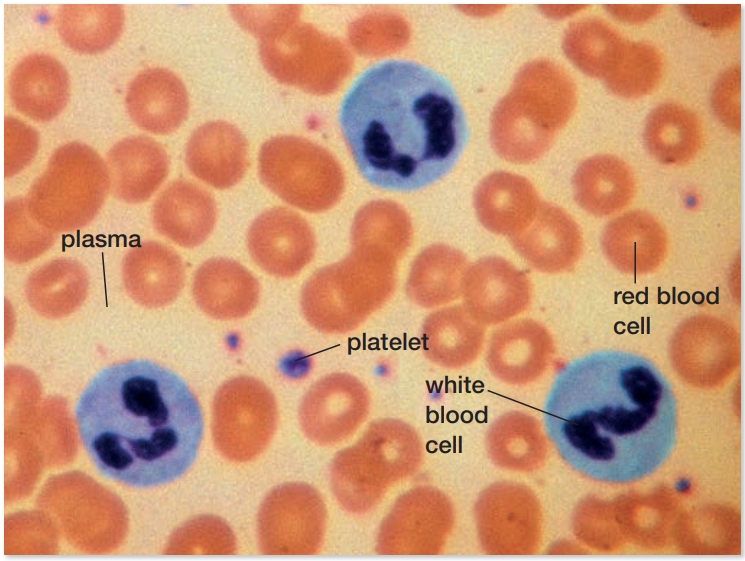
\includegraphics[scale=0.25]{Biology/1B/Images/1B-2-1.png}
    \caption{This light micrograph shows red blood cells, white blood cells and platelets.}
\end{figure}
\begin{itemize}
    \item[1.] \textbf{\underline{Plasma} (血浆):}
    \begin{itemize}
        \item Liquid part of blood ($55\%$ of blood volume).
        \item Transport:
        \begin{itemize}
            \item Digested food (e.g., glucose, amino acids).
            \item \underline{Excretory products} (排泄物 e.g., urea, carbon dioxide).
            \item Hormones.
        \end{itemize}
        \item Maintains a stable pH and regulates body temperature.
    \end{itemize}
    \item[2.] \textbf{\underline{Erythrocytes} (红细胞 Red Blood Cells):}
    \begin{itemize}
        \item Approximately 4-6 million cells per $\text{mm}^3$.
        \item Contain haemoglobin to transport oxygen.
        \item Adaptations:
        \begin{itemize}
            \item \underline{Biconcave} (双凹面) shape increases surface area.
            \item No nucleus allows more haemoglobin storage.
            \item \underline{Lifespan} (寿命) of $\sim 120$ days.
        \end{itemize}
    \end{itemize}
    \item[3.] \textbf{\underline{Leukocytes} (白细胞 White Blood Cells):}
    \begin{itemize}
        \item Approximately 4,000-11,000 cells per $\text{mm}^3$.
        \item Role:
        \begin{itemize}
            \item Defend against \underline{pathogens} (病原体 e.g., bacteria, viruses).
            \item Aid in \underline{inflammatory response} (炎症反应).
        \end{itemize}
        \item Types:
        \begin{itemize}
            \item \underline{Granulocytes} (contain granules 粒细胞 e.g., neutrophils 嗜中性粒细胞, eosinophils 嗜酸性粒细胞).
            \item \underline{Agranulocytes} (no granules 无颗粒细胞 e.g., lymphocytes 淋巴细胞, monocytes 单核细胞).
        \end{itemize}
    \end{itemize}
    \item[4.] \textbf{\underline{Platelets} (血小板):}
    \begin{itemize}
        \item Small cell \underline{fragments} (片段) without a nucleus ($\sim 150,000-400,000$ per $\text{mm}^3$).
        \item Involved in \underline{blood clotting} (凝血).
    \end{itemize}
\end{itemize}

\paragraph{Transport of Oxygen}
\begin{itemize}
    \item Haemoglobin binds oxygen in the lungs and forms \underline{oxyhaemoglobin} (氧合血红蛋白):
    \begin{equation}
        \frac{\ce{Hb + 4O2 <=> Hb.4O2}}{\ce{Haemoglobin + Oxygen <=> Oxyhaemoglobin}}
    \end{equation}
    \item Oxygen \underline{dissociation curve} (氧解离曲线):
    \begin{itemize}
        \item S-shaped curve showing \underline{haemoglobin saturation} (血红蛋白饱和度) at different oxygen pressures.
        \item In low oxygen environments, haemoglobin releases oxygen to tissues efficiently.
    \end{itemize}
    \begin{figure}[H]
        \centering
        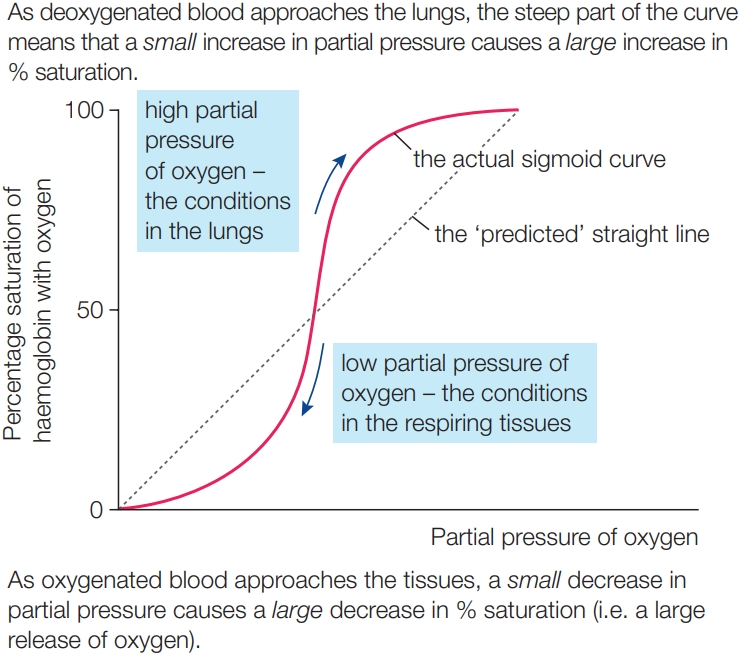
\includegraphics[scale=0.25]{Biology/1B/Images/1B-2-2.png}
        \caption{Oxygen dissociation curve for human haemoglobin.}
    \end{figure}
\end{itemize}

\paragraph{Transport of Carbon Dioxide}
\begin{itemize}
    \item Carbon dioxide is transported in three forms:
    \begin{itemize}
        \item[1.] Dissolved in plasma ($5\%$).
        \item[2.] Bound to haemoglobin as carbaminohaemoglobin ($10-20\%$).
        \item[3.] As \underline{bicarbonate ions} ($\ce{HCO3-}$ 碳酸氢根离子) in plasma ($70-85\%$, majority).
    \end{itemize}
    \item The reaction of the carbon dioxide with water is crucial. When carbon dioxide is dissolved in the blood it reacts
    slowly with the water to form carbonic acid (\ce{H2CO3}). The carbonic acid separates to form hydrogen ions (\ce{H+}) and
    hydrogencarbonate ions (\ce{HCO3-}):
    \begin{equation}
        \ce{CO2 + H2O <=> H2CO3 <=> H+ + HCO3-}
    \end{equation}
    \item \textbf{\underline{Chloride shift} (氯离子转移):} Exchange of bicarbonate ions for chloride ions in red blood cells
    maintains charge balance.
    \begin{figure}[H]
        \centering
        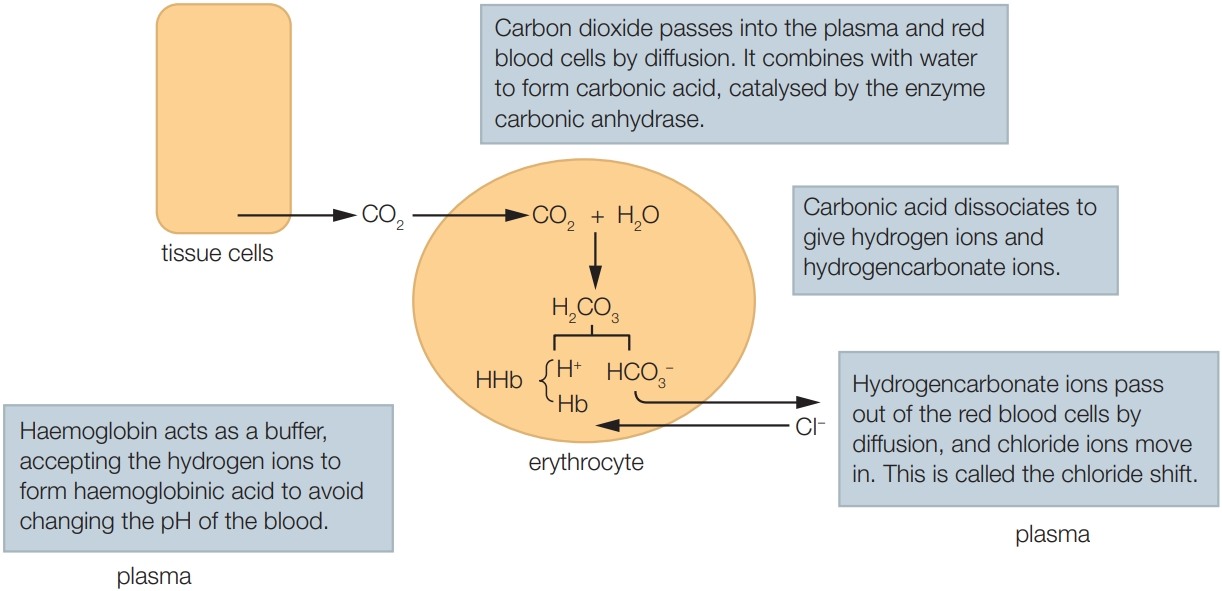
\includegraphics[scale=0.25]{Biology/1B/Images/1B-2-3.png}
        \caption{The transport of carbon dioxide from the tissues to the lungs depends on the reaction of carbon dioxide with
        water, controlled by an enzyme in the red blood cells.}
    \end{figure}
\end{itemize}

\paragraph{\underline{The Bohr Effect} (波尔效应)}
High carbon dioxide levels in active tissues lower haemoglobin's affinity for oxygen, allowing oxygen to be released more readily.
The changes in the oxygen dissociation curve that result as the carbon dioxide level changes are known as the Bohr effect.
\begin{figure}[H]
    \centering
    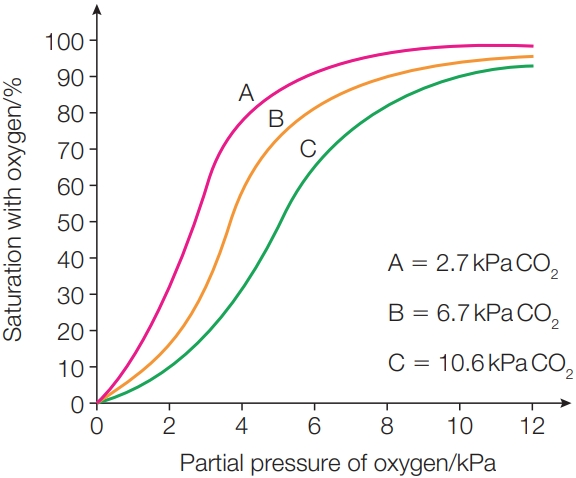
\includegraphics[scale=0.25]{Biology/1B/Images/1B-2-4.png}
    \caption{As the proportion of carbon dioxide in the environment rises, the haemoglobin curve moves down and to the right, so
    it gives up oxygen more easily. This is known as the Bohr effect.}
\end{figure}

\paragraph{\underline{Fetal Haemoglobin} (胎儿血红蛋白)}
Fetal haemoglobin has a higher oxygen affinity than adult haemoglobin, enabling oxygen transfer from the mother's blood to the
fetus.
\begin{figure}[H]
    \centering
    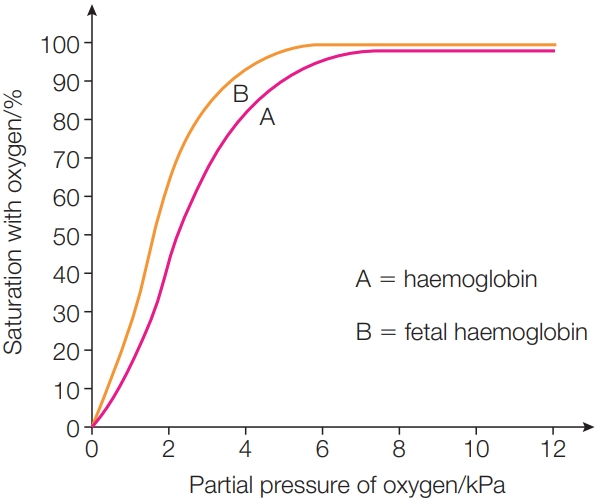
\includegraphics[scale=0.25]{Biology/1B/Images/1B-2-5.png}
    \caption{Fetal haemoglobin has a higher affi nity for oxygen than the adult haemoglobin of the mother, so it can take oxygen
    from the mother's blood and deliver it to the cells of the growing fetus.}
\end{figure}

\paragraph{\underline{Clotting} (凝血) of Blood} Blood clotting mechanism:
\begin{itemize}
    \item[1.] \underline{Platelets} (血小板) release \underline{thromboplastin} (凝血酶原) at the injury site.
    \item[2.] Thromboplastin \underline{catalyzes} (催化) the conversion of \underline{prothrombin} (凝血酶原) to
    \underline{thrombin} (凝血酶). This requires calcium ions.
    \item[3.] Thrombin converts \underline{fibrinogen} (纤维蛋白原) to \underline{fibrin} (纤维蛋白) which is insoluble.
    \item[4.] Fibrin forms a mesh that traps red blood cells and platelets, forming a \underline{clot}.
\end{itemize}
\begin{figure}[H]
    \centering
    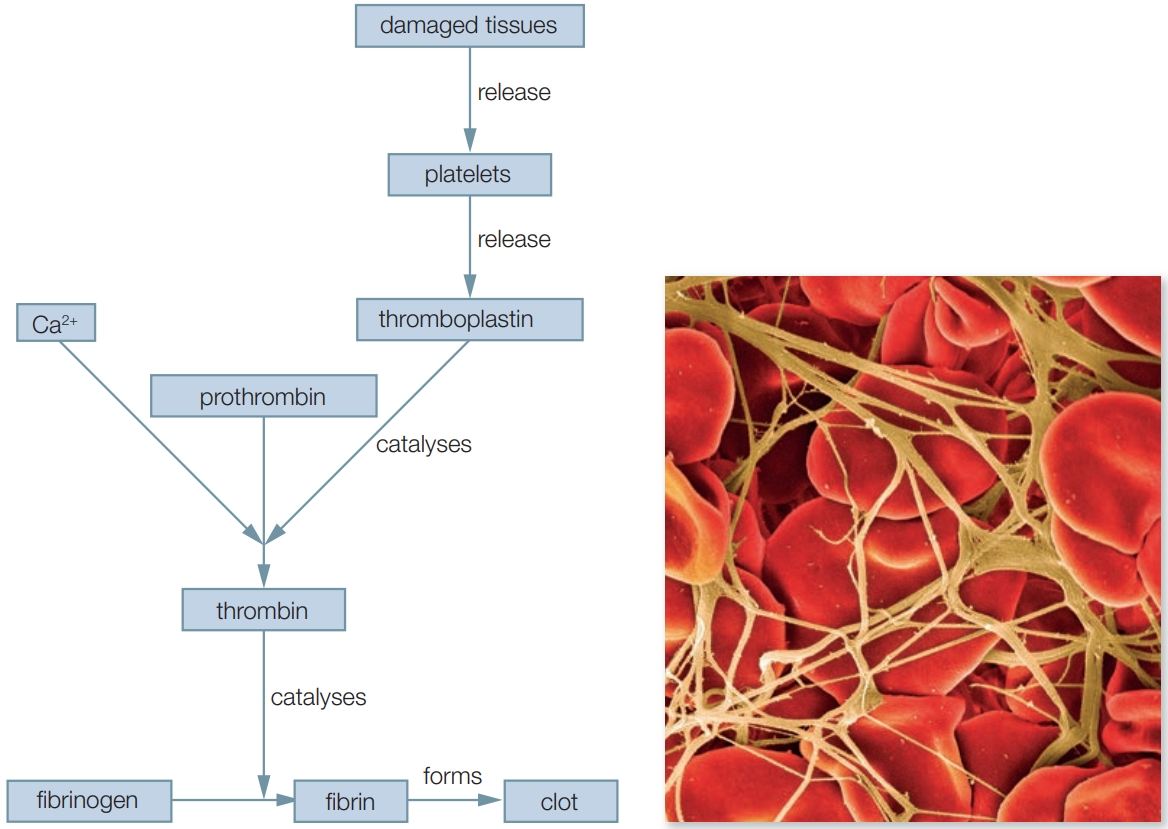
\includegraphics[scale=0.25]{Biology/1B/Images/1B-2-6.png}
    \caption{The \underline{cascade} (大量) of events that results in a life-saving or life-threatening clot. When you cut
    yourself, this is the process which seals the blood vessels and protects the delicate new tissues that form underneath.}
\end{figure}
% ==================================
%           Chapter 1B.3
%  Circulation in the Blood Vessels
%       Created by Michael Tang
%            2025.01.12
% ==================================

\subsubsection{1B.3 Circulation in the Blood Vessels}
\paragraph{Types of Blood Vessels}
\begin{itemize}
    \item[1.] \textbf{\underline{Arteries} (动脉)}
    \begin{itemize}
        \item \textbf{Function:} Carry blood away from the heart (usually \underline{oxygenated} (充满氧气的), except for
        \underline{pulmonary} (肺部) and \underline{umbilical} (脐带) arteries).
        \item \textbf{Structure:}
        \begin{itemize}
            \item Thick walls with \underline{elastic fibres} (弹性纤维), \underline{smooth muscle} (平滑肌), and
            \underline{collagen} (胶原蛋白) to \underline{withstand} (承受) high pressure.
            \item Narrow \underline{lumen} (管腔) to maintain high pressure.
        \end{itemize}
        \begin{figure}[H]
            \centering
            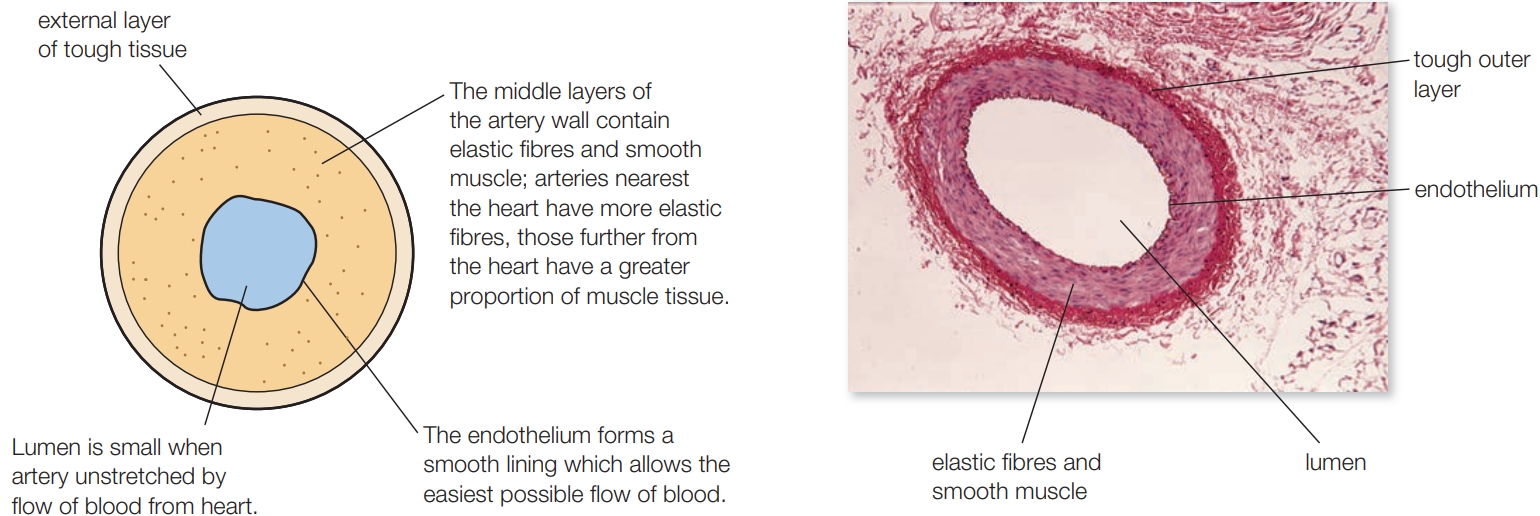
\includegraphics[scale=0.2]{Biology/1B/Images/1B-3-1.png}
            \caption{The structure of an artery means it is adapted to \underline{cope} (处理) with the \underline{surging} (涌动)
            of the blood as the heart pumps.}
        \end{figure}
        \item \textbf{Adaptations:}
        \begin{itemize}
            \item \underline{Elastic recoil} (弹性回缩) helps maintain blood flow during \underline{diastole} (舒张期).
            \item \underline{Arterioles} (小动脉) regulate blood flow to tissues by \underline{adjusting} (调整) lumen size.
        \end{itemize}
        \begin{figure}[H]
            \centering
            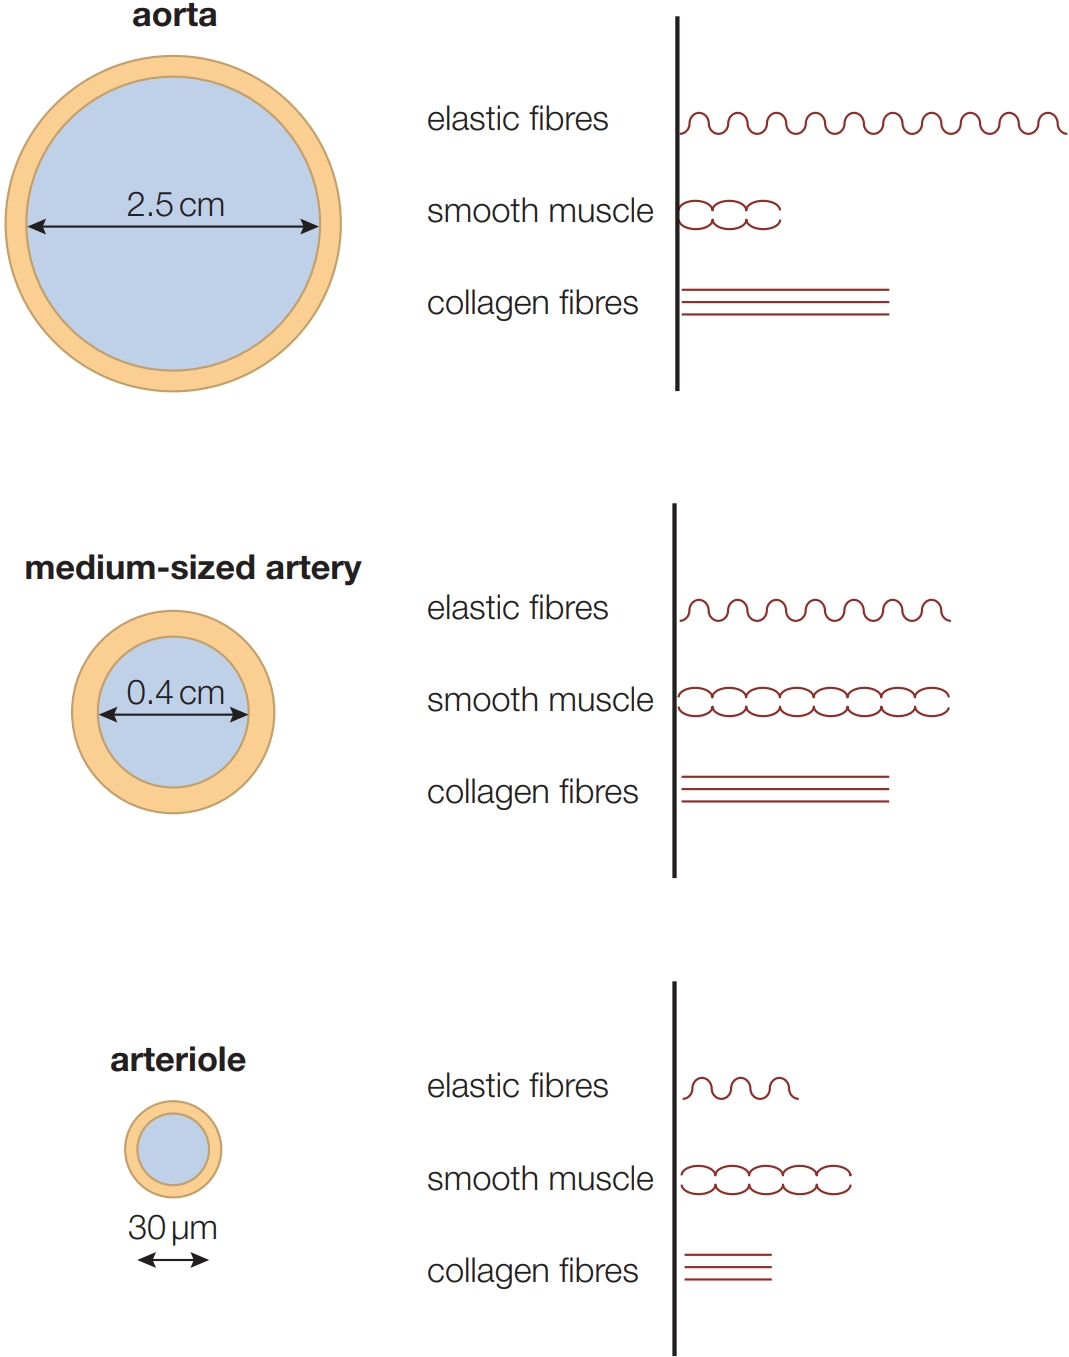
\includegraphics[scale=0.15]{Biology/1B/Images/1B-3-2.png}
            \caption{The relative proportions of different tissues in different arteries.Collagen gives general strength and
            flexibility to both arteries and veins.}
        \end{figure}
    \end{itemize}
    \item[2.] \textbf{\underline{Capillaries} (毛细血管)}
    \begin{itemize}
        \item \textbf{Function:} Facilitate exchange of substances between blood and tissues.
        \item \textbf{Structure:}
        \begin{itemize}
            \item Very thin walls (one cell thick) for efficient \underline{diffusion} (扩散).
            \item Small lumen allows red blood cells to pass through single cell, increasing contact with the
            \underline{capillary walls} (毛细血管壁).
        \end{itemize}
        \item \textbf{Adaptations:}
        \begin{itemize}
            \item Large surface area for exchange.
            \item Slow blood flow ensures more time for diffusion.
        \end{itemize}
        \begin{figure}[H]
            \centering
            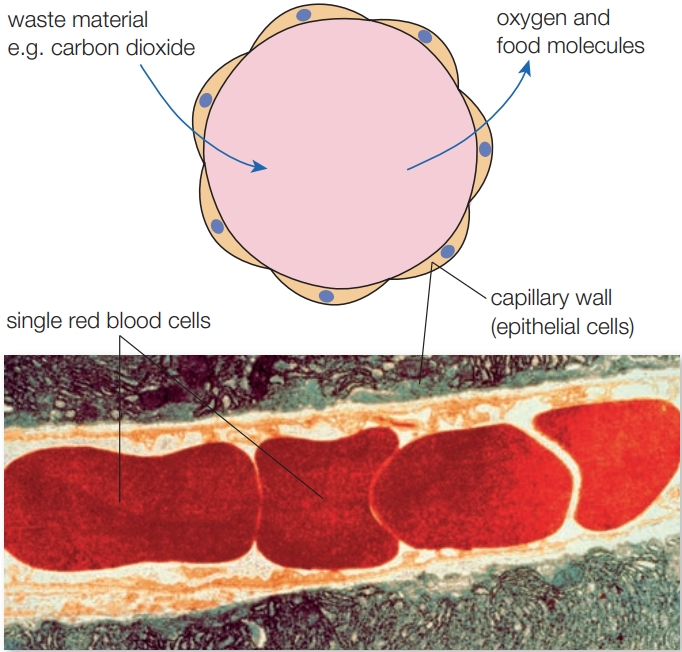
\includegraphics[scale=0.3]{Biology/1B/Images/1B-3-3.png}
            \caption{The relative proportions of different tissues in different arteries.Collagen gives general strength and
            flexibility to both arteries and veins.}
        \end{figure}
    \end{itemize}
    \item[3.] \textbf{\underline{Veins} (静脉)}
    \begin{itemize}
        \item \textbf{Function:} Carry blood back to the heart (usually \underline{deoxygenated} (缺氧的), except for pulmonary
        and umbilical veins).
        \item \textbf{Structure:}
        \begin{itemize}
            \item Thin walls with less \underline{elastic} (弹性) and muscle tissue due to lower pressure.
            \item Wide lumen to \underline{accommodate} (容纳) large volume of blood.
        \end{itemize}
        \begin{figure}[H]
            \centering
            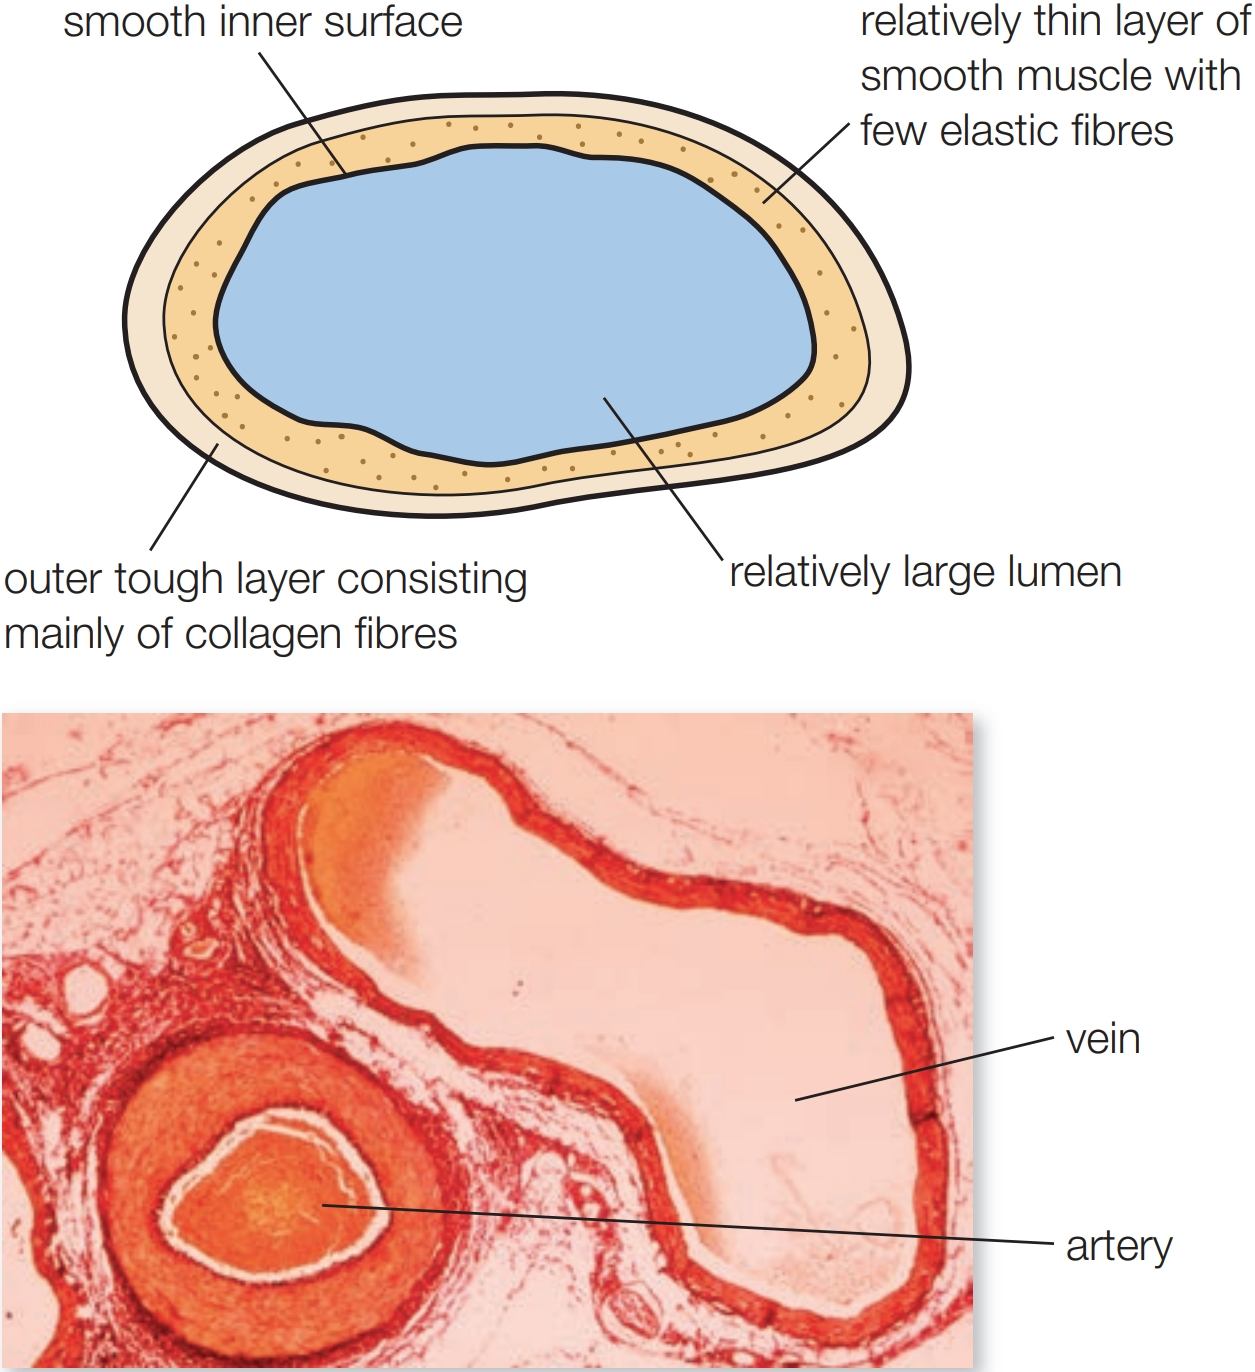
\includegraphics[scale=0.15]{Biology/1B/Images/1B-3-4.png}
            \caption{The arrangement of tissues in a vein reflects the pressure of blood in the vessel.}
        \end{figure}
    \end{itemize}
\end{itemize}

\paragraph{Key Adaptations of Blood Vessels}
\begin{itemize}
    \item \textbf{Arteries:}
    \begin{itemize}
        \item High \underline{elasticity} (弹性) for pressure \underline{surges} (涌动) from the heart.
        \item Smooth \underline{endothelium} (内皮) reduces \underline{friction} (摩擦) for efficient blood flow.
    \end{itemize}
    \begin{figure}[H]
        \centering
        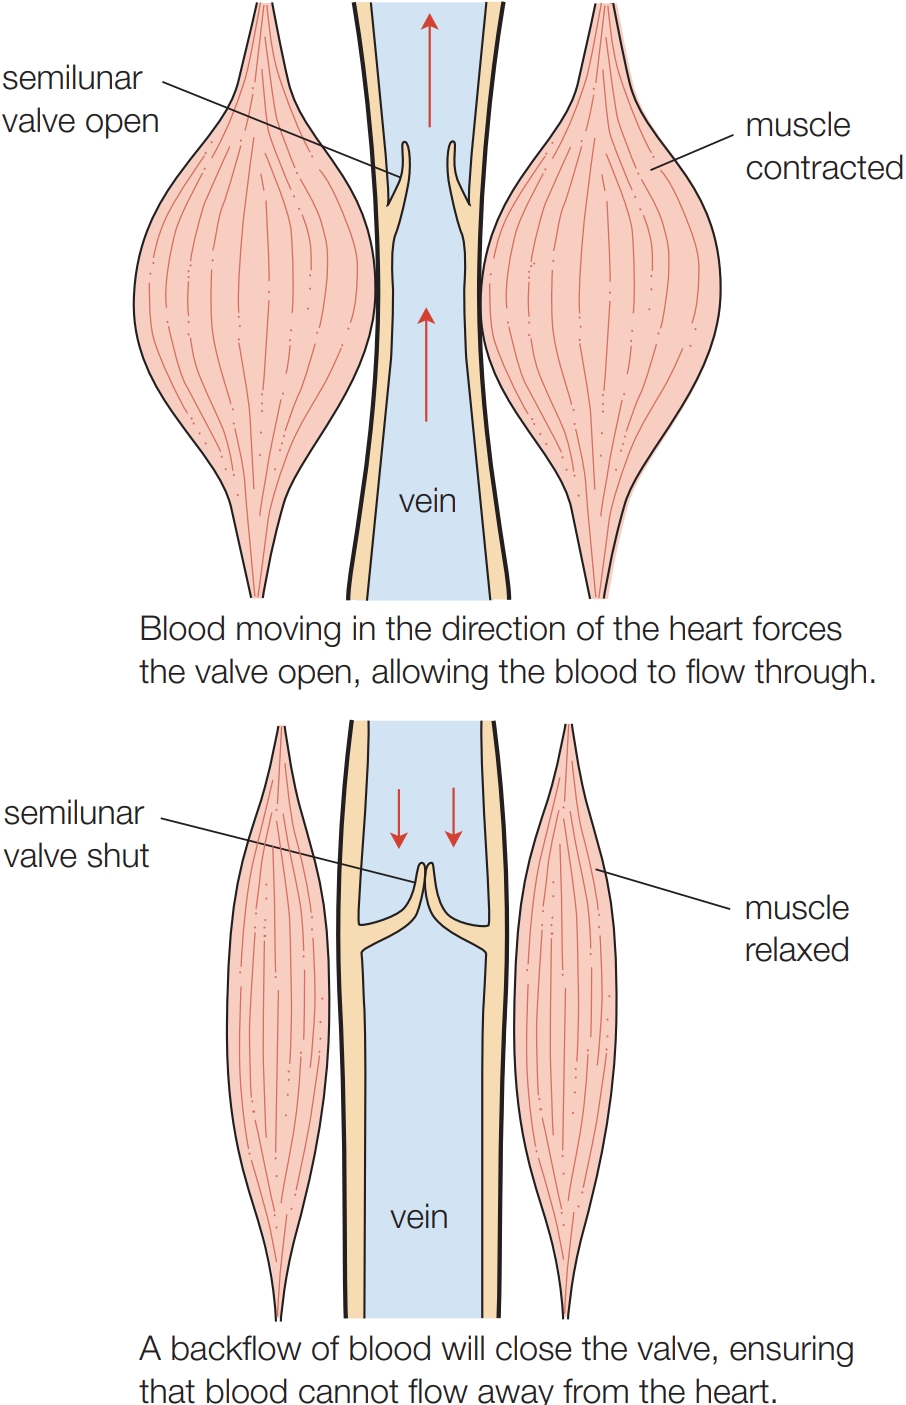
\includegraphics[scale=0.18]{Biology/1B/Images/1B-3-5.png}
        \caption{Valves in the veins make sure blood only flows in one direction - towards the heart. The contraction of large
        muscles encourages blood flow through the veins.}
    \end{figure}
    \item \textbf{Capillaries:} Short diffusion distance for gas exchange.
    \item \textbf{Veins:}
    \begin{itemize}
        \item Valves prevent backflow.
        \item Act as a \underline{reservoir} (储备) for blood (contain over 50\% of body's blood).
    \end{itemize}
\end{itemize}

\paragraph{Blood Flow Dynamics}
\begin{itemize}
    \item \textbf{Blood Pressure:} Highest in arteries, decreases in capillaries, and lowest in veins.
    \item \textbf{Velocity:} High in arteries, slows down in capillaries, and increases slightly in veins.
    \item \textbf{Surface Area:} Maximum in capillaries due to extensive branching.
\end{itemize}
\begin{figure}[H]
    \centering
    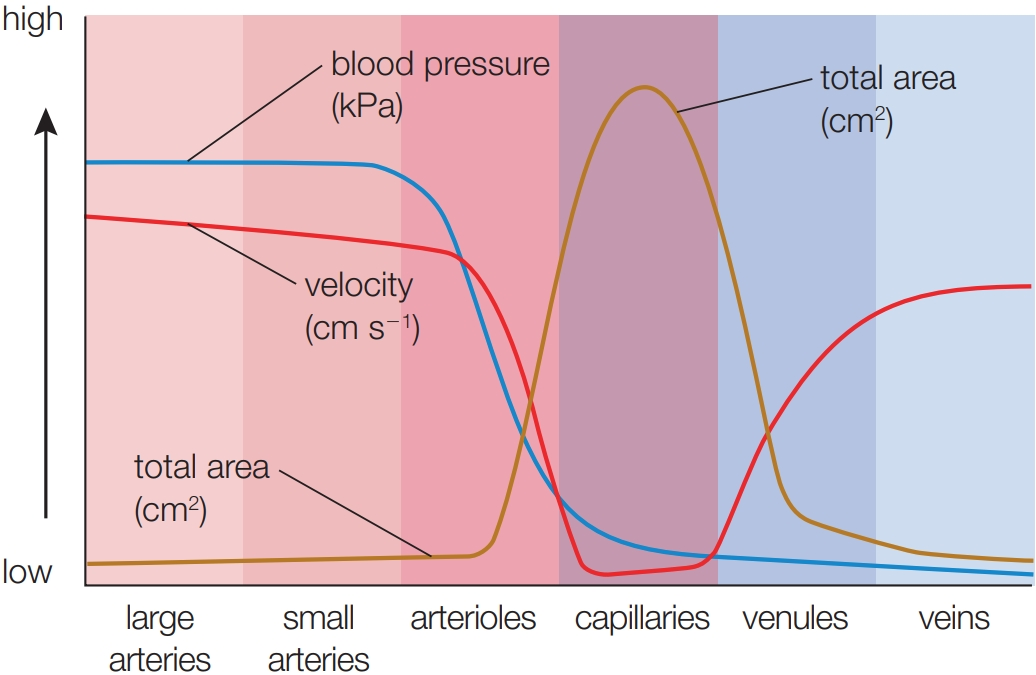
\includegraphics[scale=0.25]{Biology/1B/Images/1B-3-6.png}
    \caption{Graph to show the surface area of each major type of blood vessel in your body, along with the velocity and pressure
    of the blood travelling in them.}
\end{figure}
% ===============================
%          Chapter 1B.4
%       The Mammalian Heart
%     Created by Michael Tang
%           2025.01.12
% ===============================

\subsubsection{1B.4 The Mammalian Heart}
\paragraph{Structure of the Heart}
\begin{itemize}
    \item[1.] \textbf{General Description:}
    \begin{itemize}
        \item The heart is a \underline{four-chambered organ} (四腔器官) located in the \underline{thorax} (胸腔).
        \item Functions as a double pump to circulate oxygenated and deoxygenated blood.
        \item Composed of \underline{cardiac muscle} (心肌, specialized for continuous contraction without \underline{fatigue}
        疲倦).
    \end{itemize}
    \item[2.] \textbf{Chambers:}
    \begin{itemize}
        \item \textbf{\underline{Right Atrium} (右心房):} Recieves deoxygenated blood from the body via the \underline{vena cava}
        (腔静脉).
        \item \textbf{\underline{Right Ventricle} (右心室):} Pumps deoxygenated blood to the lungs via the \underline{pulmonary
        artery} (肺动脉).
        \item \textbf{\underline{Left Atrium} (左心房):} Recieves oxygenated blood from the lungs via the \underline{pulmonary
        vein} (肺静脉).
        \item \textbf{\underline{Left Ventricle} (左心室):} Pumps oxygenated blood to the body via the \underline{aorta} (主动脉).
        It has thicker walls than the right ventricle to withstand higher pressure.
    \end{itemize}
    \item[3.] \textbf{Key Structure:}
    \begin{itemize}
        \item \textbf{\underline{Septum} (隔膜):} Thick muscular wall seperating the left and right sides of the heart.
        \item \textbf{\underline{Valves} (瓣膜):} Prevent backflow of blood:
        \begin{itemize}
            \item \textbf{\underline{Tricuspid Valve} (三尖瓣):} Between the right atrium and ventricle.
            \item \textbf{\underline{Bicuspid (Mitral) Valve} (二尖瓣):} Between the left atrium and ventricle.
            \item \textbf{\underline{Semilunar Valves} (半月瓣):} At the exit of the pulmonary artery and aorta.
        \end{itemize}
        \item \textbf{\underline{Tendineae Cords} (腱索 Chordae Tendineae):} Prevent valves from inverting under pressure.
    \end{itemize}
    \item[4.] \textbf{\underline{Coronary Circulation} (冠状循环):}
    \begin{itemize}
        \item The heart muscle is supplied with oxygenand nutrients by the \underline{coronary arteries} (冠状动脉).
        \item Rich in \underline{myoglobin} (肌红蛋白), a \underline{respiratory pigment} (呼吸色素) with a higher oxygen
        \underline{affinity} (亲和力) than hemoglobin.
    \end{itemize}
    \begin{figure}[H]
        \centering
        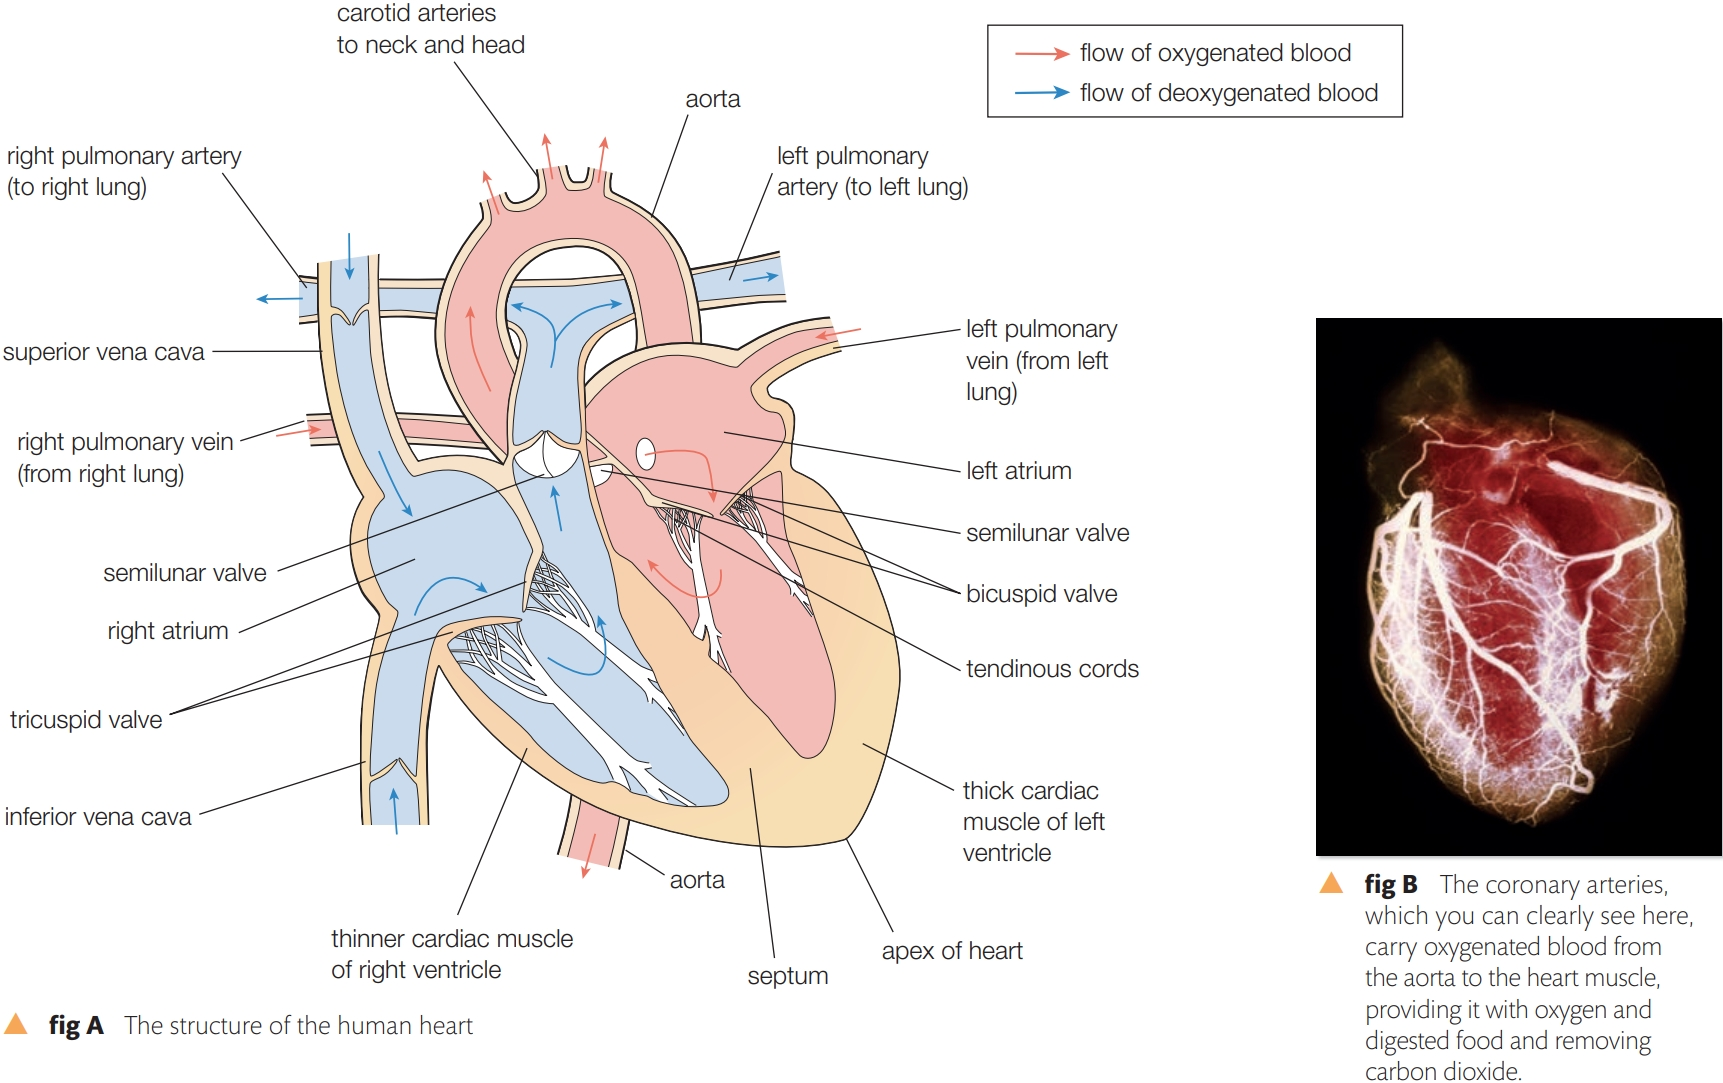
\includegraphics[scale=0.25]{Biology/1B/Images/1B-4-1.png}
    \end{figure}
\end{itemize}

\paragraph{Action of the Heart}
\begin{itemize}
    \item \textbf{Blood Flow Sequence:}
    \begin{itemize}
        \item[1.] \textbf{Deoxygenated Blood:}
        \begin{itemize}
            \item Enters the right atrium via the \underline{vena cava} (腔静脉).
            \item Flows into the left ventricle through the \underline{tricuspid valve} (三尖瓣).
            \item Is pumped to the body through the aorta.
        \end{itemize}
        \item[2.] \textbf{Oxygenated Blood:}
        \begin{itemize}
            \item Returns from the lungs to the left atrium via the \underline{pulmonary vein} (肺静脉).
            \item Flows into the left ventricle through the \underline{bicuspid valve} (二尖瓣).
            \item Is pumped to the body through the aorta.
        \end{itemize}
    \end{itemize}
    \item \textbf{Valve Function:}
    \begin{itemize}
        \item Valves open and close due to pressure difference to ensure \underline{unidirectional flow} (单向流动).
        \item Semilunar valves prevent backflow from arteries to ventricles.
        \item \underline{Atrioventricular valves} (房室瓣) prevent backflow from ventricles to atria.
    \end{itemize}
    \item \textbf{Pressure Adaptation:}
    \begin{itemize}
        \item The left ventricle has a thicker muscular wall to pump blood at higher pressure to the \underline{systemic circuit}
        (体循环).
        \item The right ventricle pumps blood at lower pressure to the lungs to avoid damaging the delicate capillaries.
    \end{itemize}
\end{itemize}

\paragraph{The Cardiac Cycle}
\begin{itemize}
    \item \textbf{Phases:}
    \begin{itemize}
        \item \textbf{\underline{Atrial Systole} (心房收缩):} Atria contract, forcing blood into the ventricles.
        \item \textbf{\underline{Ventricular Systole} (心室收缩):} Ventricles contract, pumping blood to the lungs and body.
        \item \textbf{\underline{Diastole} (舒张期):} Both atria and ventricles relax, allowing chambers to fill with blood.
    \end{itemize}
    \item \textbf{Heartbeat Sounds:}
    \begin{itemize}
        \item \textbf{\underline{'Lub' Sound} (第一心音):} Closing of atrioventricular valves during ventricular systole.
        \item \textbf{\underline{'Dub' Sound} (第二心音):} Closing of semilunar valves during ventricular diastole.
    \end{itemize}
    \item \textbf{Cycle Duration:} Each cardiac cycle lasts approximately 0.8 seconds in humans:
    \begin{itemize}
        \item Atrial systole: 0.1 seconds.
        \item Ventricular systole: 0.3 seconds.
        \item Diastole: 0.4 seconds.
    \end{itemize}
    \begin{figure}[H]
        \centering
        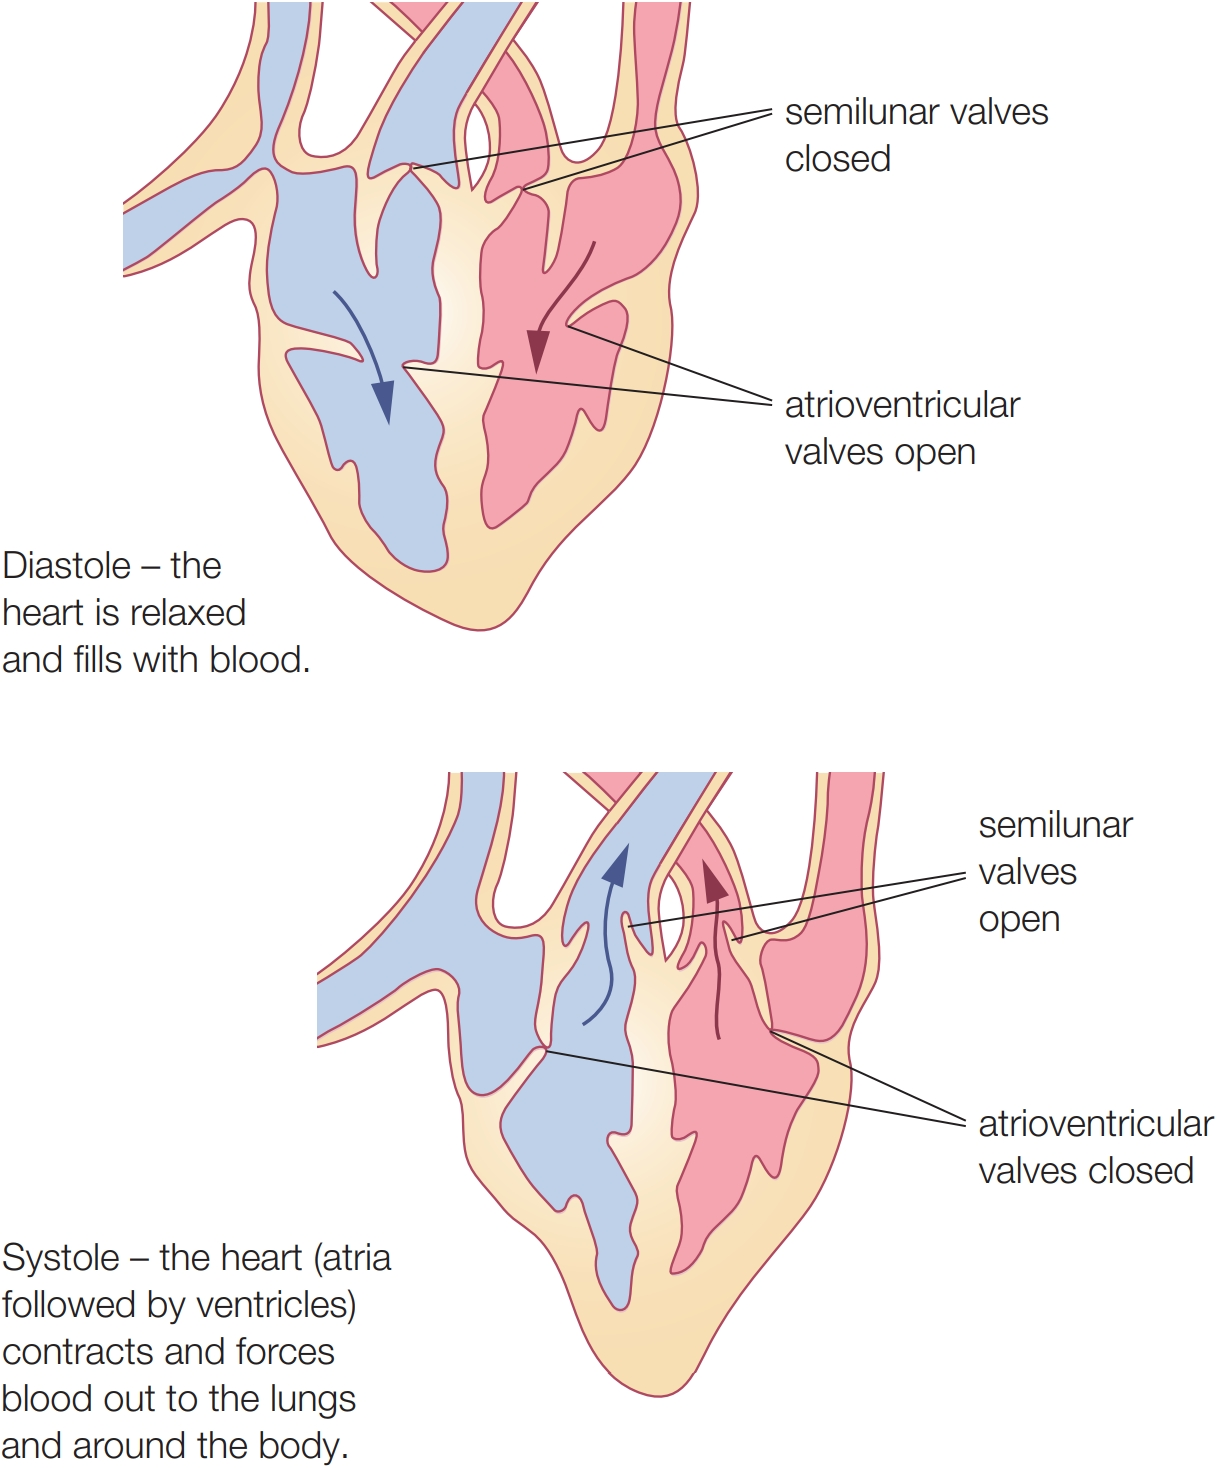
\includegraphics[scale=0.15]{Biology/1B/Images/1B-4-2.png}
        \caption{The cardiac cycle.}
    \end{figure}
\end{itemize}
% ===============================
%          Chapter 1B.5
%        Atherosclerosis
%     Created by Michael Tang
%           2025.01.13
% ===============================

\subsubsection{1B.5 Atherosclerosis}
\paragraph{Overview}
\begin{itemize}
    \item \underline{Cardiovascular diseases} (CVDs 心血管病) are the leading cause of death globally, responsible for 31\% of all
    global deaths (according to WHO data, 2017).
    \item Many CVDs are associated with \underline{atherosclerosis} (动脉粥样硬化), a condition where \underline{plaques} (斑块)
    build up inside arteries.
\end{itemize}

\paragraph{Atherosclerosis}
\begin{itemize}
    \item \textbf{Definition:} A desease where plaques (fatty deposits) from in arteries, narrowing the lumen and reducing blood
    flow.
    \item \textbf{Development:}
    \begin{itemize}
        \item \textbf{Step 1:} Damage to the \underline{endothelium} (内皮 e.g., due to high blood pressure or smoking).
        \item \textbf{Step 2:} \underline{Inflammatory response} (炎症反应); white blood cells migrate to the area.
        \item \textbf{Step 3:} \underline{Accumulation} (积累) of \underline{cholesterol} (胆固醇), forming a \underline{fatty
        deposit} (atheroma 脂肪沉积).
        \item \textbf{Step 4:} Calcium salts and fibrous tissue build up around the atheroma, forming a hardened plaque.
    \end{itemize}
    \item \textbf{Effects:}
    \begin{itemize}
        \item Narrowed arteries increase blood pressure.
        \item Increased risk of blood clots (\underline{thrombosis} 血栓形成) at the site of plaques.
    \end{itemize}
    \begin{figure}[H]
        \centering
        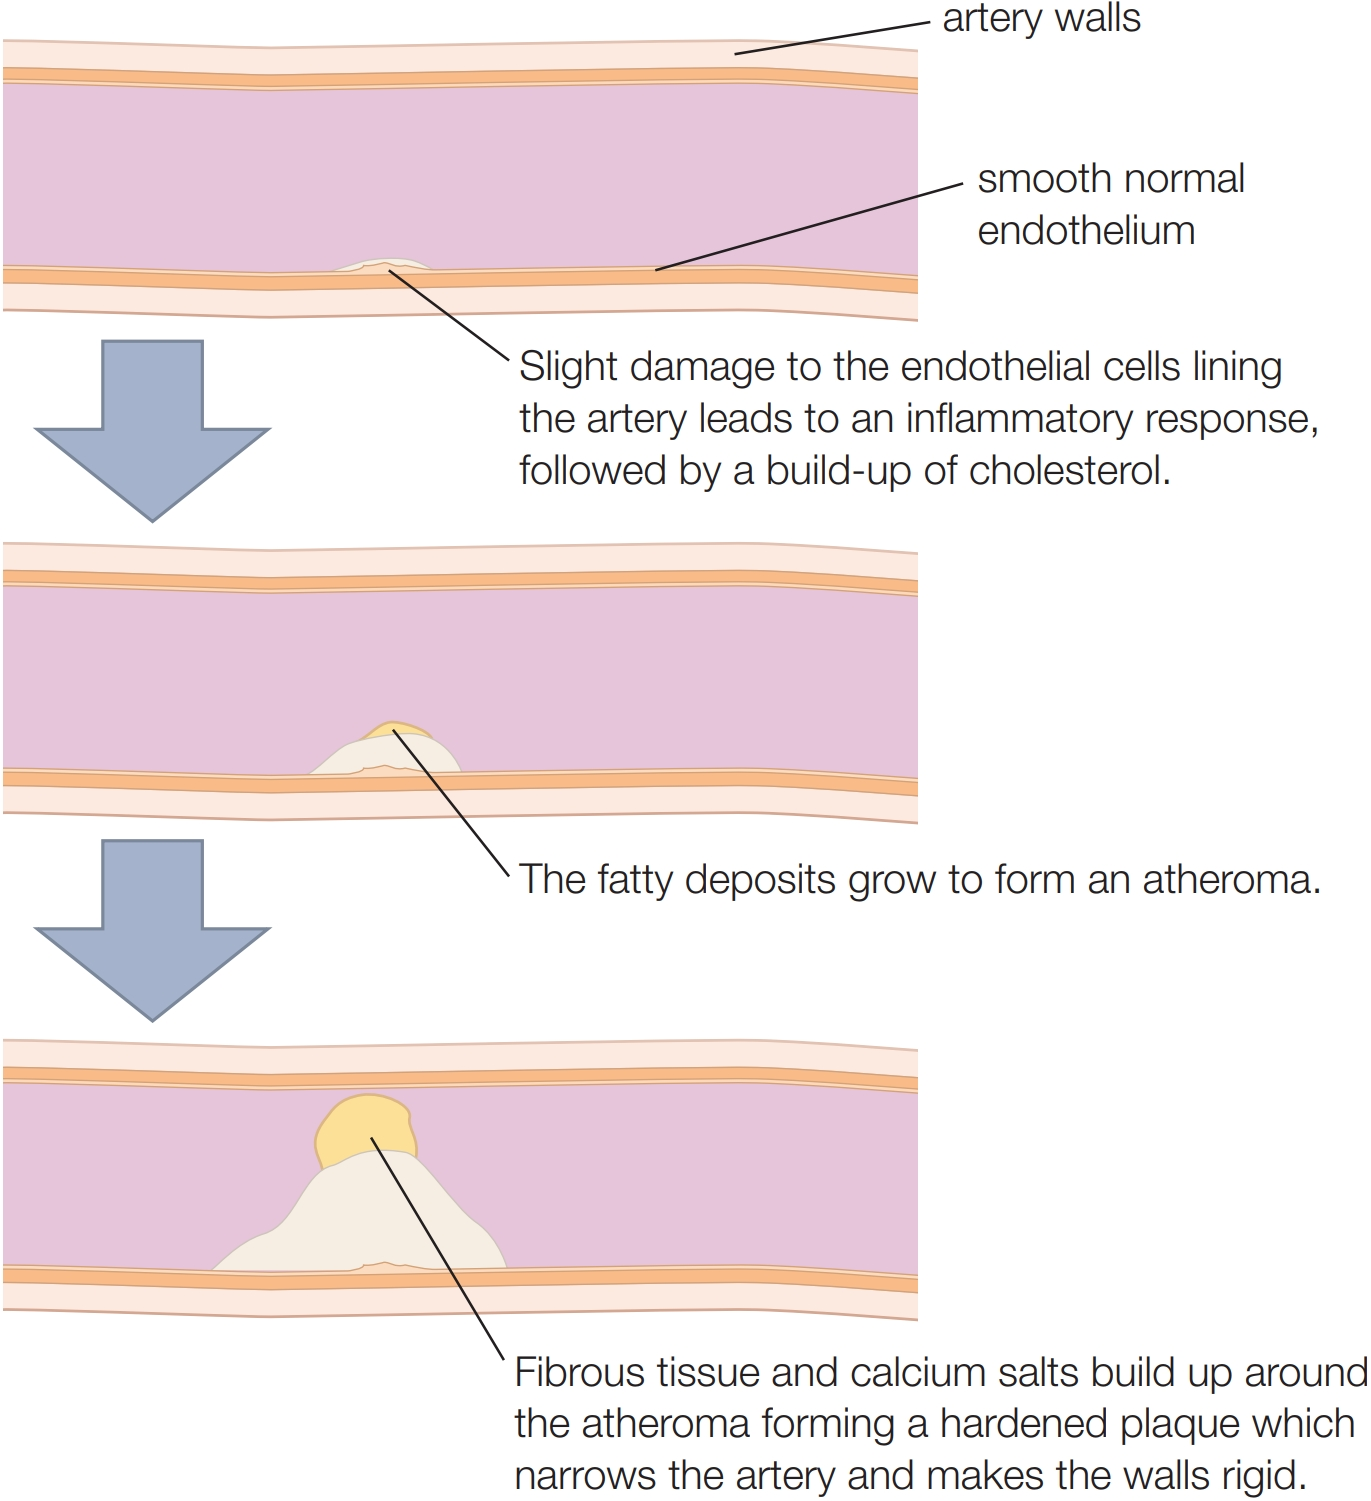
\includegraphics[scale=0.18]{Biology/1B/Images/1B-5-1.png}
        \caption{The development of atherosclerosis.}
    \end{figure}
\end{itemize}

\paragraph{Health Impacts of Atherosclerosis}
\begin{itemize}
    \item[1.] \textbf{\underline{Aneurysms} (动脉瘤):}
    \begin{itemize}
        \item Weakening of arterial walls due to plaque formation.
        \item The artery may \underline{bulge} (凸出) and \underline{rupture} (破裂), causing internal bleeding.
        \item Common in the aorta or brain arteries.
    \end{itemize}
    \item[2.] \textbf{\underline{Rised Blood Pressure} (高血压):}
    \begin{itemize}
        \item Narrowed arteries force the heart to pump harder.
        \item High blood pressure damages organs like the \underline{kidneys} (肾脏), eyes, and brain.
    \end{itemize}
    \item[3.] \textbf{Heart Diseases:}
    \begin{itemize}
        \item \textbf{\underline{Angina} (心绞痛):}
        \begin{itemize}
            \item Reduced blood flow to the heart muscle due to narrowed \underline{coronary arteries} (冠状动脉).
            \item Symptoms include chest pain, especially during exercise.
        \end{itemize}
        \item \textbf{\underline{Myocardial Infarction} (心肌梗死 Heart Attack):}
        \begin{itemize}
            \item Complete blockage of a coronary artery.
            \item Starves part of the heart muscle of oxygen, causing tissue death.
            \item Severity depends on the location and \underline{extent} (程度) of blockage.
        \end{itemize}
        \begin{figure}[H]
            \centering
            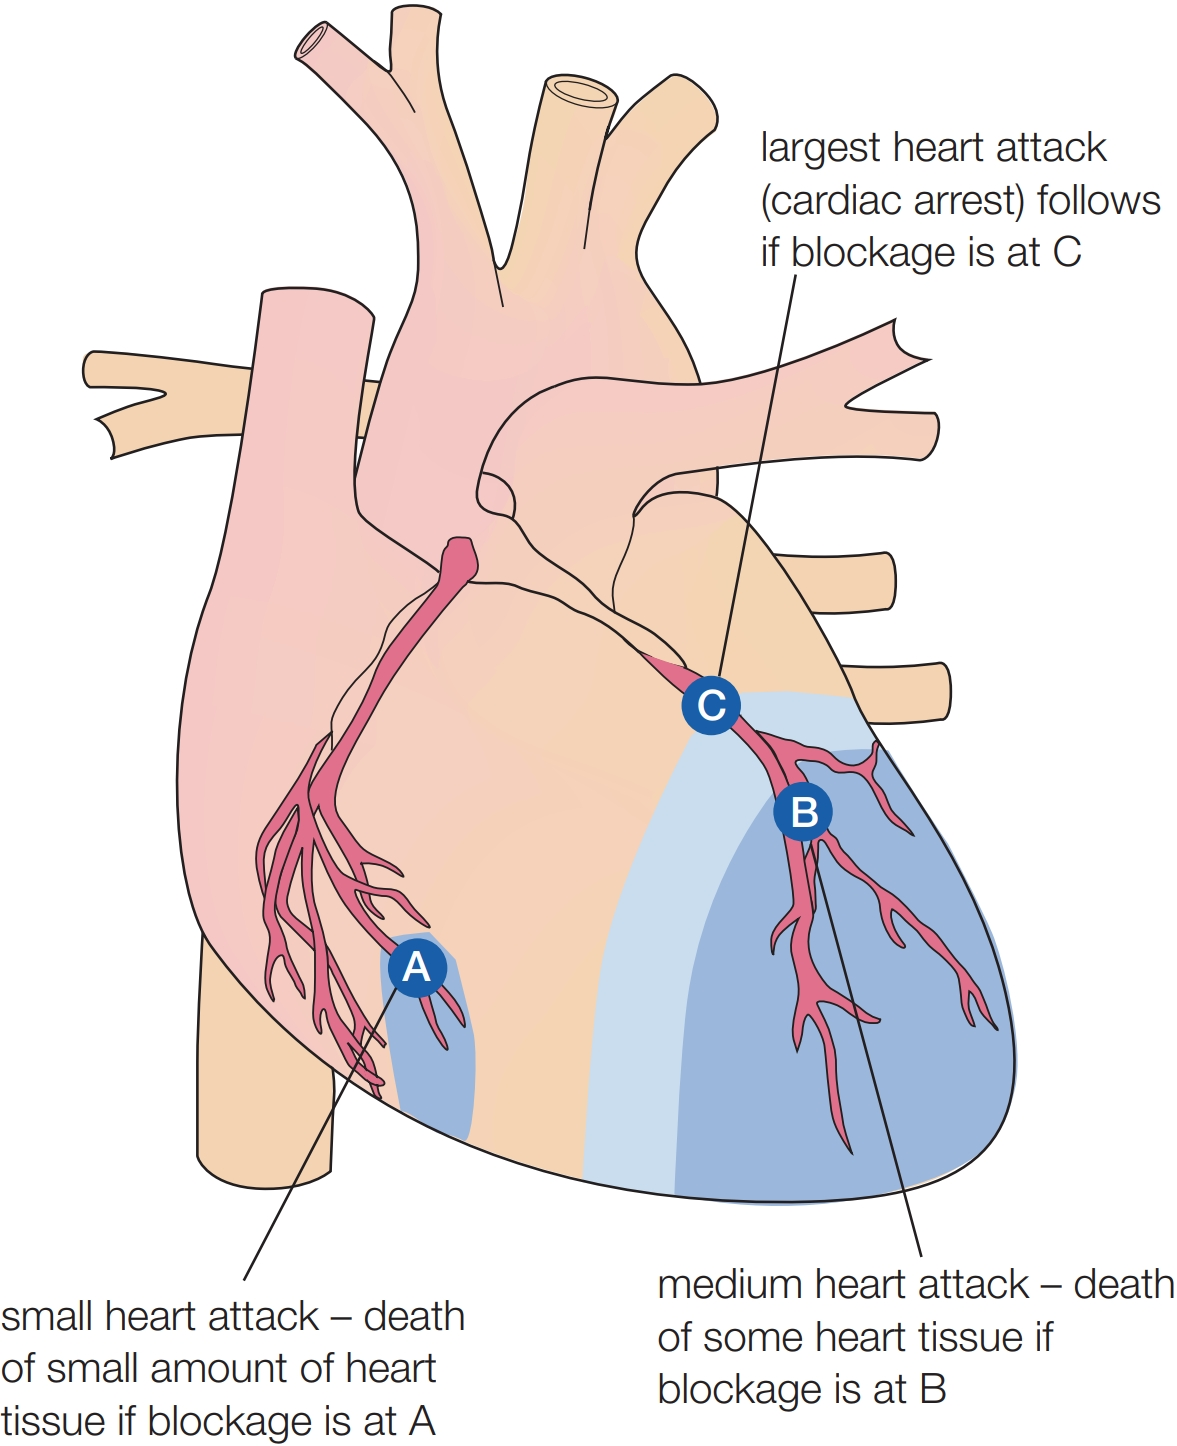
\includegraphics[scale=0.18]{Biology/1B/Images/1B-5-2.png}
            \caption{The size and severity of a heart attack is closely related to the position of the blockage in the coronary
            artery.}
        \end{figure}
    \end{itemize}
    \item[4.] \textbf{\underline{Stroke} (中风):}
    \begin{itemize}
        \item Disruption of blood supply to the brain due to a clot or \underline{hemorrhage} (出血).
        \item Symptoms include \underline{dizziness} (头晕), \underline{slurred speech} (口齿不清), and \underline{paralysis} (瘫痪).
        \item Quick treatment with \underline{clot-busting drugs} (溶栓药) increases survival chances.
    \end{itemize}
\end{itemize}

\paragraph{Prevention and Treatment}
\begin{itemize}
    \item \textbf{Prevention:}
    \begin{itemize}
        \item Regular exercise.
        \item Healthy diet low in saturated fats.
        \item Avoiding smoking and managing blood pressure.
    \end{itemize}
    \item \textbf{Treatment:}
    \begin{itemize}
        \item \textbf{Medication:} E.g., Statins (降脂药, lower cholesterol levels), \underline{antihypertensives} (降压药).
        \item \textbf{Surgery:} E.g., \underline{angioplasty} (血管成形术) to widen arteries, \underline{bypass surgery} (搭桥手术),
        \underline{stent insertion} (支架植入).
    \end{itemize}
\end{itemize}
\subsection{Cardiovascular Health and Rick}
% ===============================
%          Chapter 1C.1
%  Risk, Correlation, and Cause
%     Created by Michael Tang
%           2025.01.13
% ===============================

\subsubsection{1C.1 Risk, Correlation, and Cause}
\paragraph{What is Risk?}
\begin{itemize}
    \item \textbf{Definition:}
    \begin{itemize}
        \item Risk is the probability of an event occurring.
        \item Example: The probability of picking a blue ball from a bag of six colored balls is 1 in 6, 0.1666, or 16.7\%.
    \end{itemize}
    \item \textbf{How Risk is Rerceived:}
    \begin{itemize}
        \item Perception is influenced by:
        \begin{itemize}
            \item Familiarity with the activity.
            \item Enjoyment of the activity.
            \item Approval or disapproval of the activity.
        \end{itemize}
        \item Actual mathematical risk may differ from personal perception.
        \item Example: Risk of dying in a car accident is 1 in 5747, but many people fear flying more than driving.
    \end{itemize}
\end{itemize}

\paragraph{\underline{Epidemiology} (流行病学) and Risk Factors}
\begin{itemize}
    \item \textbf{Epidemiology:}
    \begin{itemize}
        \item The study of disease patterns and their causes in populations.
        \item Identifies risk factors that increase the likelihood of disease.
    \end{itemize}
    \item \textbf{Risk Factors:}
    \begin{itemize}
        \item Factors that increase the probability of developing a diesase (e.g., smoking, obesity, and lack of exercise).
        \item Diseases like atherosclerosis are termed multifactorial disease as they result from multiple interacting factors.
    \end{itemize}
    \item \textbf{Correlation vs. Causation:}
    \begin{itemize}
        \item \textbf{\underline{Correlation} (相关性):} Two sets of data change together but do not imply cause and effect.
        \item \textbf{\underline{Causation} (因果关系):} A direct cause-effect relationship is established.
    \end{itemize}
\end{itemize}

\paragraph{Obesity and Cardiovascular Disease}
\begin{itemize}
    \item \textbf{Impact of Obesity:} Increased risk of diabetes and cardiovascular disease.
    \item \textbf{Why People Stay Obese:}
    \begin{itemize}
        \item Overestimation of benefits or underestimation of risks of unhealthy behaviors.
        \item Enjoyment of certain activities or foods.
        \item Lack of motivation or understanding of the risks.
    \end{itemize}
\end{itemize}
% ==================================
%           Chapter 1C.2
%  Investigating the Causes of CVDs
%      Created by Michael Tang
%            2025.01.13
% ==================================

\subsubsection{1C.2 Investigating the Causes of CVDs}
\paragraph{Designing Studies}
\begin{itemize}
    \item \textbf{Purpose:}
    \begin{itemize}
        \item Investigate one factor or variable while controlling others.
        \item Larger sample sizes yield more statistically significant results.
    \end{itemize}
    \item \textbf{Longitudinal Studies:} Follow the same group of individuals over many years to observe long-term patterns.
    \item \textbf{Meta-Analysis:} Combines results from multiple studies for more reliable data.
\end{itemize}

\paragraph{Designing and Evaluating Studies}
\begin{itemize}
    \item \textbf{Key Criteria:}
    \begin{itemize}
        \item \textbf{Valid:} The study answers the questions it sets out to address.
        \item \textbf{Precise:} Measurements are consistent and have little variation.
        \item \textbf{Reliable:} Results can be reproduced by other scientists.
    \end{itemize}
    \item \textbf{Factors Affecting Reliability:}
    \begin{itemize}
        \item Who funded the study?
        \item Were measurements biased or affected by external interests?
    \end{itemize}
    \item \textbf{Importance:} Evaluation ensures practical applications in health and research are based on \underline{robust}
    (坚固的) evidence.
\end{itemize}

\paragraph{Risk Factors for Cardiovascular Diseases (CVDs)}
\textbf{Non-Modifiable Risk Factors:}
\begin{itemize}
    \item \textbf{Genetics:}
    \begin{itemize}
        \item \underline{Inherited tendency} (遗传趋势) for heart disease.
        \item Example: Twin studies show a higher likelihood of heart disease in identical twins than \underline{fraternal}
        (兄弟的) twins.
    \end{itemize}
    \item \textbf{Age:} Older individuals have reduced \underline{elasticity} (弹性) in arteries, leading to higher CVD risk.
    \item \textbf{Gender:}
    \begin{itemize}
        \item Men are more likely to develop CVDs than \underline{pre-menopausal women} (绝经前妇女).
        \item \underline{Oestrogen} (雌性激素) in women reduces plaque build-up, offering some protection before
        \underline{menopause} (绝经期).
    \end{itemize}
\end{itemize}
% =========================================
%              Chapter 1C.3
%  Risk Factors for Cardiovascular Disease
%          Created by Michael Tang
%               2025.01.13
% =========================================

\subsubsection{1C.3 Risk Factors for Cardiovascular Disease}
\paragraph{Cardiovascular Disease Overview}
\begin{itemize}
    \item \textbf{Definition:} Diseases affecting the heart and blood vessels.
    \item \textbf{Global Impact:}
    \begin{itemize}
        \item Account for 31\% of global deaths (WHO data, 2017).
        \item Significant causes include atherosclerosis.
    \end{itemize}
\end{itemize}

\paragraph{Atherosclerosis}
\begin{itemize}
    \item \textbf{Process:}
    \begin{itemize}
        \item Damage to \underline{endothelium} (内皮细胞) due to high pressure or smoking.
        \item \underline{Inflammatory} (炎症性的) response $\rightarrow$ Cholesterol accumulates forming an atheroma.
        \item Atheromas harden into plaques causing artery narrowing and reduced \underline{elasticity} (弹性).
    \end{itemize}
    \item \textbf{Effects:}
    \begin{itemize}
        \item Increased blood pressure.
        \item Risks of \underline{aneurysms} (颅内动脉瘤), \underline{angina} (心绞痛), \underline{myocardial infarction} (心肌梗死),
        and stroke.
    \end{itemize}
\end{itemize}

\paragraph{Heart Disease}
\begin{itemize}
    \item \textbf{Angina:}
    \begin{itemize}
        \item Chest pain from restricted blood flow to the heart.
        \item Triggered by \underline{anaerobic respiration} \footnote{\textbf{Anaerobic Respiration} Anaerobic respiration is the
        breakdown of glucose without oxygen to release energy. It occurs in the \underline{cytoplasm} (细胞质) of cells and
        produces less ATP compared to aerobic respiration.
        \textbf{Process:}
        \begin{itemize}
            \item \textbf{In Animals:}
            \begin{itemize}
                \item Glucose $\rightarrow$ \underline{Lactic Acid} (乳酸) + Energy (ATP).
                \item Reaction Formula:
                \begin{equation}
                    \ce{C6H12O6 -> 2C3H6O3 + ATP}
                \end{equation}
                \item Key Point: Lactic acid builds up and can cause muscle \underline{fatigue} (劳累) during
                \underline{strenuous} (费力的) activities.
            \end{itemize}
            \item \textbf{In Plants and \underline{Yeast} (酵母):}
            \begin{itemize}
                \item Glucose $\rightarrow$ \underline{Ethanol} (乙醇) + Carbon Dioxide + Energy (ATP).
                \item Reaction Formula:
                \begin{equation}
                    \ce{C6H12O6 -> 2C2H5OH + 2CO2 + ATP}
                \end{equation}
                \item Key Point: Ethanol is produced and used in the production of alcoholic beverages.
            \end{itemize}
        \end{itemize}} (无氧呼吸) in \underline{cardiac muscles} (心肌).
    \end{itemize}
    \item \textbf{Myocardial Infarction (Heart Attack):}
    \begin{itemize}
        \item Complete blockage of \underline{coronary arteries} (冠状动脉) $\rightarrow$ Heart muscle is
        \underline{oxygen-deprived} (氧气供应不足).
        \item Severe cases lead to \underline{cardiac arrest} (心脏骤停) and death.
    \end{itemize}
\end{itemize}

\paragraph{Stroke}
\begin{itemize}
    \item \textbf{Cause:} Interruption of blood supply to the brain (clot or \underline{rupture} 破裂).
    \item \textbf{Symptoms:} Dizziness, speech issues, \underline{numbness} (麻木) on one side.
    \item \textbf{Survival:} Quick medical intervention significantly increases recovery chances.
\end{itemize}

\paragraph{Risk Factors}
\begin{itemize}
    \item \textbf{Non-Modifiable Risk Factors:}
    \begin{itemize}
        \item \textbf{Age:} Increased risk as blood vessels lose elasticity.
        \item \textbf{Gender:}
        \begin{itemize}
            \item Males at higher risk.
            \item Females post-menopause are at increased risk due to reduced \underline{oestrogen} (雌性激素) levels.
        \end{itemize}
        \item \textbf{Genetics:} Family history of CVD or inheritable artery weakness.
    \end{itemize}
    \item \textbf{Modifiable Risk Factors:}
    \begin{itemize}
        \item \textbf{Smoking:}
        \begin{itemize}
            \item Increases plaque formation.
            \item Damages \underline{endothelium} (内皮细胞) and narrows arteries.
        \end{itemize}
    \end{itemize}
\end{itemize}
% =========================================
%              Chapter 1C.4
%      Diet and Cardiovascular Health
%          Created by Michael Tang
%               2025.02.13
% =========================================

\subsubsection{1C.4 Diet and Cardiovascular Health}
\paragraph{Weight Issues and CVD Risk}
\begin{itemize}
    \item \textbf{Obesity and CVDs:} Obesity, often caused by consuming more food than the body needs, increases the risk of
    cardiovascular diseases (CVDs) due to the \underline{accumulation} (积累) of \underline{excess} (过量的) fat.
    \item \textbf{BMI and Obesity:} The Body Mass Index (BMI) is commonly used to measure obesity. It is calculated as the
    following equation.
    \begin{equation}
        \text{BMI} = \frac{\text{Weight (kg)}}{\text{Height}^2 (\text{m}^2)}
    \end{equation}
\end{itemize}

\paragraph{Measuring Healthy Weight}
\begin{itemize}
    \item \textbf{BMI Classification for Adults:}
    \begin{itemize}
        \item Underweight: BMI $< 18.5 \text{kg}/\text{m}^2$
        \item Ideal weight: $18.5 \leq \text{BMI} < 25 \text{kg}/\text{m}^2$
        \item Overweight: $25 \leq \text{BMI} < 30 \text{kg}/\text{m}^2$
        \item Obese: BMI $\geq 30 \text{kg}/\text{m}^2$
        \item Severely obese: BMI $\geq 40 \text{kg}/\text{m}^2$
    \end{itemize}
    \item \textbf{\underline{Waist-to-Hip Ratio} (WHR 腰臀比):}
    \begin{itemize}
        \item \textbf{Waist size:} measured at the navel (肚脐) level.
        \item \textbf{Hip size:} measured at the widest part of the hips.
        \item \textbf{Indicator of Obesity:}
        \begin{itemize}
            \item \textbf{Male:} WHR $> 0.9$ indicates obesity.
            \item \textbf{Female:} WHR $> 0.85$ indicates obesity.
        \end{itemize}
        \item A high WHR indicates a higher risk of CVDs.
    \end{itemize}
\end{itemize}

\paragraph{BMI Limitations in Predicting CVD Risk}
\begin{itemize}
    \item \textbf{Muscle vs. Fat:} BMI doesn't account for muscle mass. Athletes or muscular individuals might be classified as
    overweight or obese even if they are healthy.
    \item \textbf{Genetic Variation:} People metabolize fats differently, and some can maintain a healthy balance of LDLs
    (Low-Density Lipoproteins 低密度脂蛋白) and HDLs (High-Density Lipoproteins 高密度脂蛋白) despite higher body fat.
\end{itemize}

\paragraph{\underline{Cholesterol} (胆固醇) and CVD Risk}
\begin{itemize}
    \item \textbf{LDL (Low-Density Lipoproteins):} Carry cholesterol from the liver to the cells. High LDL levels lead to plaque
    buildup in arteries, increasing the risk of CVD.
    \item \textbf{HDL (High-Density Lipoproteins):} Transport cholesterol from cells to the liver for disposal. Higher HDL levels
    reduce CVD risk.
    \item \textbf{Ideal LDL:HDL Ratio:} Around 3:1 (LDL:HDL).
\end{itemize}

\paragraph{Diet, Fat, and CVDs}
\begin{itemize}
    \item \textbf{Saturated Fats:} Linked to high cholesterol levels and increased risk of CVDs. Countries with high saturated
    fat intake (from animal fats) have higher heart disease rates.
    \item \textbf{Correlation between Fat Intake and CVDs:} Diets high in animal fats (mainly saturated fats) are associated with
    an increase in CVDs.
\end{itemize}

% =================================================
%                  Chapter 1C.5
%  Dietary Antioxidants and Cardiovascular Disease
%             Created by Michael Tang
%                   2025.02.13
% =================================================

\subsubsection{1C.5 Dietary Antioxidants and Cardiovascular Disease}
\paragraph{\underline{Antioxidants} (防老化) and Heart Health}
\begin{itemize}
    \item \textbf{Antioxidants:} Compounds found in fruits and vegetables that may reduce oxidative stress, which can contribute
    to CVDs.
    \item \textbf{Fruit and Vegetables:} Eating 5 or more portions of fruits and vegetables per day is linked to a lower risk of
    coronary heart disease (CVD), as seen in data from a longitudinal study.
    \item \textbf{Vitamin C:} An antioxidant known for its role in connective tissue and blood vessel health. It helps protect
    against damage in the arteries. A deficiency in vitamin C can lead to a higher risk of heart disease, as the body's blood
    vessels are more prone to damage.
\end{itemize}

\paragraph{Conflicting Evidence in Antioxidant Research}
\begin{itemize}
    \item Early studies suggested antioxidants like vitamin C could prevent heart disease.
    \item \textbf{Conflicting Evidence:} A major study in 2016 concluded that there was no clear relationship between vitamin C
    intake and heart health. It even showed that taking vitamin C supplements might damage heart health.
\end{itemize}

\paragraph{Testing for Vitamin C}
\begin{itemize}
    \item A simple laboratory test can be used to measure vitamin C in foods. The test uses a reagent called \underline{DCPIP}
    (2,6-Dichlorophenolindophenol 二氯酚靛酚, \ce{C12H7Cl2NO2}), which turns colorless when it reacts with vitamin C.
    \item The volume of DCPIP used indicates the concentration of vitamin C in the sample.
    \item \textbf{Application:} The test can be used to compare the vitamin C content in different foods
\end{itemize}
% =========================================
%              Chapter 1C.6
%           Using the Evidence
%          Created by Michael Tang
%               2025.02.13
% =========================================

\subsubsection{1C.6 Using the Evidence}
\paragraph{Prevention is Better Than Cure}
\begin{itemize}
    \item CVDs cost individuals, families, and society a lot in terms of healthcare and lost productivity.
    \item Prevention is more cost-effective than treatment. Healthy habits can prevent the need for expensive medical
    \underline{interventions} (干预).
\end{itemize}

\paragraph{Overweight or Underweight}
\begin{itemize}
    \item Being overweight or underweight both increase the risk of CVDs.
    \item Regular physical activity helps protect against CVDs by improving cardiovascular fitness. The more oxygen used during
    exercise, the lower the CVD risk.
\end{itemize}

\paragraph{Smoking and CVD Risk}
\begin{itemize}
    \item Smoking is one of the leading risk factors for CVD. Smokers are at a higher risk of developing heart disease. Research
    shows that people who quit smoking after 1 year see a significant reduction in their heart disease risk.
    \item \textbf{Global Smoking Statistics:} In the UAE, 21.9\% of people are smokers, with higher rates among men (24.8\%) than
    women (4.2\%).
\end{itemize}

\paragraph{Obesity and CVDs}
\begin{itemize}
    \item Obesity is linked to a higher risk of developing CVDs due to increased fat storage, which can lead to health
    \underline{complications} (并发症) like \underline{hypertension} (高血压) and \underline{poor blood circulation} (血液循环不良).
    \item \textbf{Diet and Exercise:} Eating a balanced diet and exercising regularly can help maintain a healthy weight and
    reduce the risk of obesity and related heart diseases.
\end{itemize}

\paragraph{Salt and CVDs}
In many developed countries, excessive salt intake is linked to high blood pressure and CVDs. Reducing salt intake globally could
lower blood pressure and the incidence of CVDs.

\paragraph{Lifestyle Choices and Perception of Risk}
\begin{itemize}
    \item \textbf{Risk Perception:} People often miscalculate the risks of smoking, high-fat diets, and lack of exercise.
    Immediate rewards (e.g., pleasure from eating high-fat food) may be prioritized over long-term health risks.
    \item \textbf{Psychological Factors:} The habit of smoking or eating unhealthy food may be hard to break, even if people know
    the risks.
\end{itemize}

\paragraph{Global Public Health Efforts}
Governments and health organizations spend billions on campaigns to reduce smoking and promote healthy diets. However, some argue
this spending might be a waste if individuals don't change their behavior.
% =========================================
%              Chapter 1C.7
%    The Benefits and Risks of Treatment
%          Created by Michael Tang
%               2025.02.13
% =========================================

\subsubsection{1C.7 The Benefits and Risks of Treatment}
\paragraph{Controlling Blood Pressure (Antihypertensives 降压药)}
\begin{itemize}
    \item Hypertension (high blood pressure) is a major risk factor for CVDs.
    \item Antihypertensive drugs help lower blood pressure and prevent complications.
\end{itemize}

\paragraph{Types of Antihypertensive Drugs}
\begin{itemize}
    \item[1.] \textbf{\underline{Diuretics} (利尿剂):} Increase urine output, removing excess fluids and salts, reducing blood
    volume and lowering blood pressure.
    \item[2.] \textbf{\underline{Beta-blockers} ($\beta$-受体阻滞剂):} Reduce the effects of \underline{adrenaline} (肾上腺素),
    slowing the heart rate and making contractions less forceful.
    \item[3.] \textbf{\underline{Symphathetic Nervous Inhibitors} (交感神经系统抑制剂):} Prevent nerve signals that cause arteries
    to \underline{constrict} (收缩), keeping arteries relaxed.
    \item[4.] \textbf{\underline{ACE Inhibitors} (ACE 抑制剂):} Block the production of angiotensin (a hormone that constricts
    blood vessels 血管紧张素), keeping blood pressure low.
\end{itemize}

\paragraph{Risks of Antihypertensive Drugs}
\begin{itemize}
    \item If not monitored properly, blood pressure may drop too low, causing falls, dizziness, and \underline{fainting} (晕厥).
    \item \textbf{\underline{Side Effects} (副作用):} \underline{Swelling} (肿胀), tiredness, fatigue, \underline{constipation}
    (便秘).
    \item \textbf{\textbf{Compliance Issue} (服从性问题):} Patients may stop taking medication due to side effects, ignoring the 
    greater but invisible risk of CVDs.
\end{itemize}

\paragraph{Statins (Cholesterol-Lowering Drugs 他汀类药物 / 降胆固醇药物)}
\begin{itemize}
    \item Statins reduce blood cholesterol levels, particularly LDLs (bad cholesterol), while increasing HDLs (good cholesterol).
    \item \textbf{Function}
    \begin{itemize}
        \item Block the enzyme in the liver responsible for cholesterol production.
        \item Reduce \underline{inflammation} (发炎) in the arteries, preventing plaque buildup.
    \end{itemize}
    \item \textbf{Effectiveness}
    \begin{itemize}
        \item Statins significantly reduce the risk of CVDs across different groups (e.g., smokers, diabetics, elderly).
        \item Greatest effect seen in diabetics and smokers.
    \end{itemize}
    \item \textbf{Risks}
    \begin{itemize}
        \item Common side effects: Muscle/joint aches, \underline{nausea} (恶心), \underbar{constipation} (便秘), and
        \underline{diarrhea} (腹泻).
        \item Rare but serious risks:
        \begin{itemize}
            \item Muscle inflammation (can be fatal).
            \item Liver damage (very rare but possible).
        \end{itemize}
    \end{itemize}
    \item \textbf{Long-Term Effects (UK Study)}
    \begin{itemize}
        \item Over 5 years, statin users had a lower risk of heart attacks and death.
        \item Protection lasted up to 10 years after stopping the drug.
    \end{itemize}
\end{itemize}

\paragraph{\underline{Plant Stanols} (植物甾烷醇 / 植物固醇) and Sterols}
\begin{itemize}
    \item Found in spreads and yoghurts, similar in structure to cholesterol.
    \item Reduce LDL absorption in the blood, lowering heart disease risk by \~25\%.
    \item Not as rigorously tested as statins, but still beneficial in a healthy diet.
\end{itemize}

\paragraph{\underline{Anticoagulants} (抗凝血药) and Platelet Inhibitors (Preventing Blood Clots)}
\begin{itemize}
    \item Used after surgery or for people at risk of blood clots (thrombosis 血栓形成).
    \item Prevent blood clotting too easily, reducing heart attack and stroke risk.
    \item \textbf{Types}
    \begin{itemize}
        \item \underline{Anticoagulants} (抗凝血药, e.g., \underline{Warfarin} (华法林))
        \begin{itemize}
            \item Interferes with \underline{prothrombin} (凝血酶原 / 凝血素) production, preventing clot formation.
            \item \textbf{Risk:} If not monitored, internal bleeding can occur.
        \end{itemize}
        \item \underline{Platelet Inhibitory Drugs} (血小板抑制剂, e.g., \underline{Aspirin} (阿司匹林), \underline{Clopidogrel}
        (氯吡格雷))
        \begin{itemize}
            \item Prevent platelets from sticking together, reducing clot risk.
            \item \textbf{Risk:} Can cause stomach \underline{irritation} (刺激) and bleeding.
        \end{itemize}
    \end{itemize}
    \item \textbf{Balancing Risks and Benefits}
    \begin{itemize}
        \item Combination of aspirin + clopidogrel can reduce CVD risk by 20-25\%.
        \item However, it increases the risk of serious bleeding.
        \begin{itemize}
            \item \textbf{In high-risk patients:} 5 cardiovascular events avoided per 1000 treated, but 3 major bleeds occur.
            \item \textbf{In low-risk patients:} 23 cardiovascular events avoided, but 10 major bleeds occur.
        \end{itemize}
    \end{itemize}
\end{itemize}

\section{Membranes, Proteins, DNA, Gene Expression}
\subsection{Membranes and Transport}
% ===============================
%          Chapter 2A.1
%         Cell Membranes
%     Created by Michael Tang
%           2025.02.14
% ===============================

\subsubsection{2A.1 Cell Membranes}
\paragraph{Cell Membranes and Their Functions}
\begin{itemize}
    \item \textbf{Cell Membrane:} Forms the outer boundary of a cell, controlling what enters and exits.
    \item \textbf{Membranes in Cells:} Found around \underline{organelles} \footnote{\textbf{Organelle:} An organelle is a
    specialized structure within a cell that performs a specific function. Examples include the nucleus (with contains genetic
    material), mitochondria (which produce energy), and the \underline{endoplasmic reticulum} (内质网, which hepls in protein and
    lipid synthesis). Organelles are often surrounded by membranes to \underline{compartmentalize} (划分) their functions within
    the cell.} (细胞器) like the nucleus and \underline{mitochondria} (线粒体).
    \item \textbf{Functions of Cell Membranes}
    \begin{itemize}
        \item Act as barriers, maintaining different conditions inside and outside the cell.
        \item Hold enzymes for reactions (e.g., respiration in mitochondria).
        \item Allow \underline{vesicles} (囊泡) to transport and secrete substances.
    \end{itemize}
\end{itemize}

\paragraph{The Structure of Membranes}
\begin{itemize}
    \item Composed of \underline{phospholipids} (磷脂) and proteins arranged in a specific way.
    \item \textbf{\underline{Phospholipid Bilayer} (磷酸双分子层)}
    \begin{itemize}
        \item \textbf{Phospholipid Molecule:}
        \begin{itemize}
            \item \textbf{\underline{Hydrophilic head} (亲水头):} Attracted to water, faces outwards.
            \item \textbf{\underline{Hydrophobic tail} (疏水尾):} Repelled by water, faces inwards.
        \end{itemize}
        \begin{figure}[H]
            \centering
            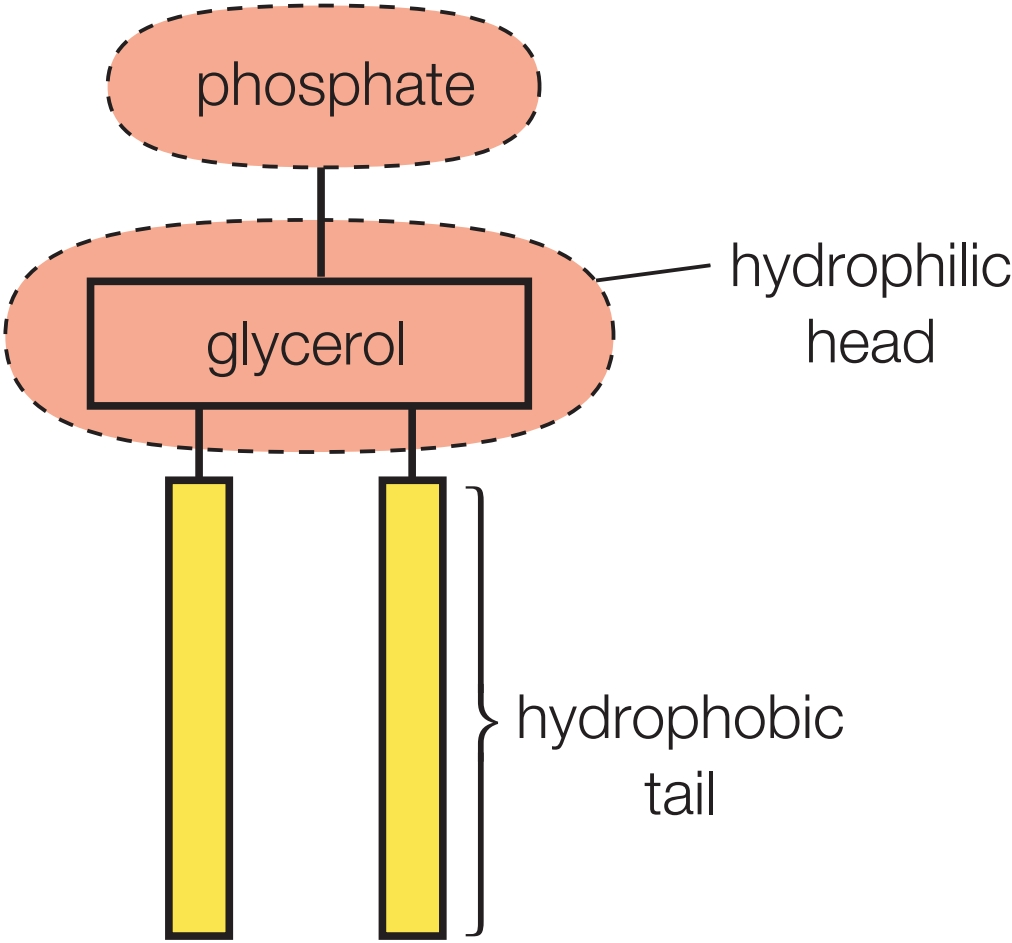
\includegraphics[scale=0.12]{Biology/2A/Images/2A-1-1.png}
            \caption{A phospholipid molecule.}
        \end{figure}
        \item In water, phospholipids self-assemble:
        \begin{itemize}
            \item \textbf{\underline{Monolayer} (单分子层):} At air / water interface.
            \item \textbf{\underline{Bilayer} (双分子层):} Hydrophilic heads outward, hydrophobic tails inward.
            \item \textbf{\underline{Micelle} (胶束):} Spherical structure in water.
        \end{itemize}
        \begin{figure}[H]
            \centering
            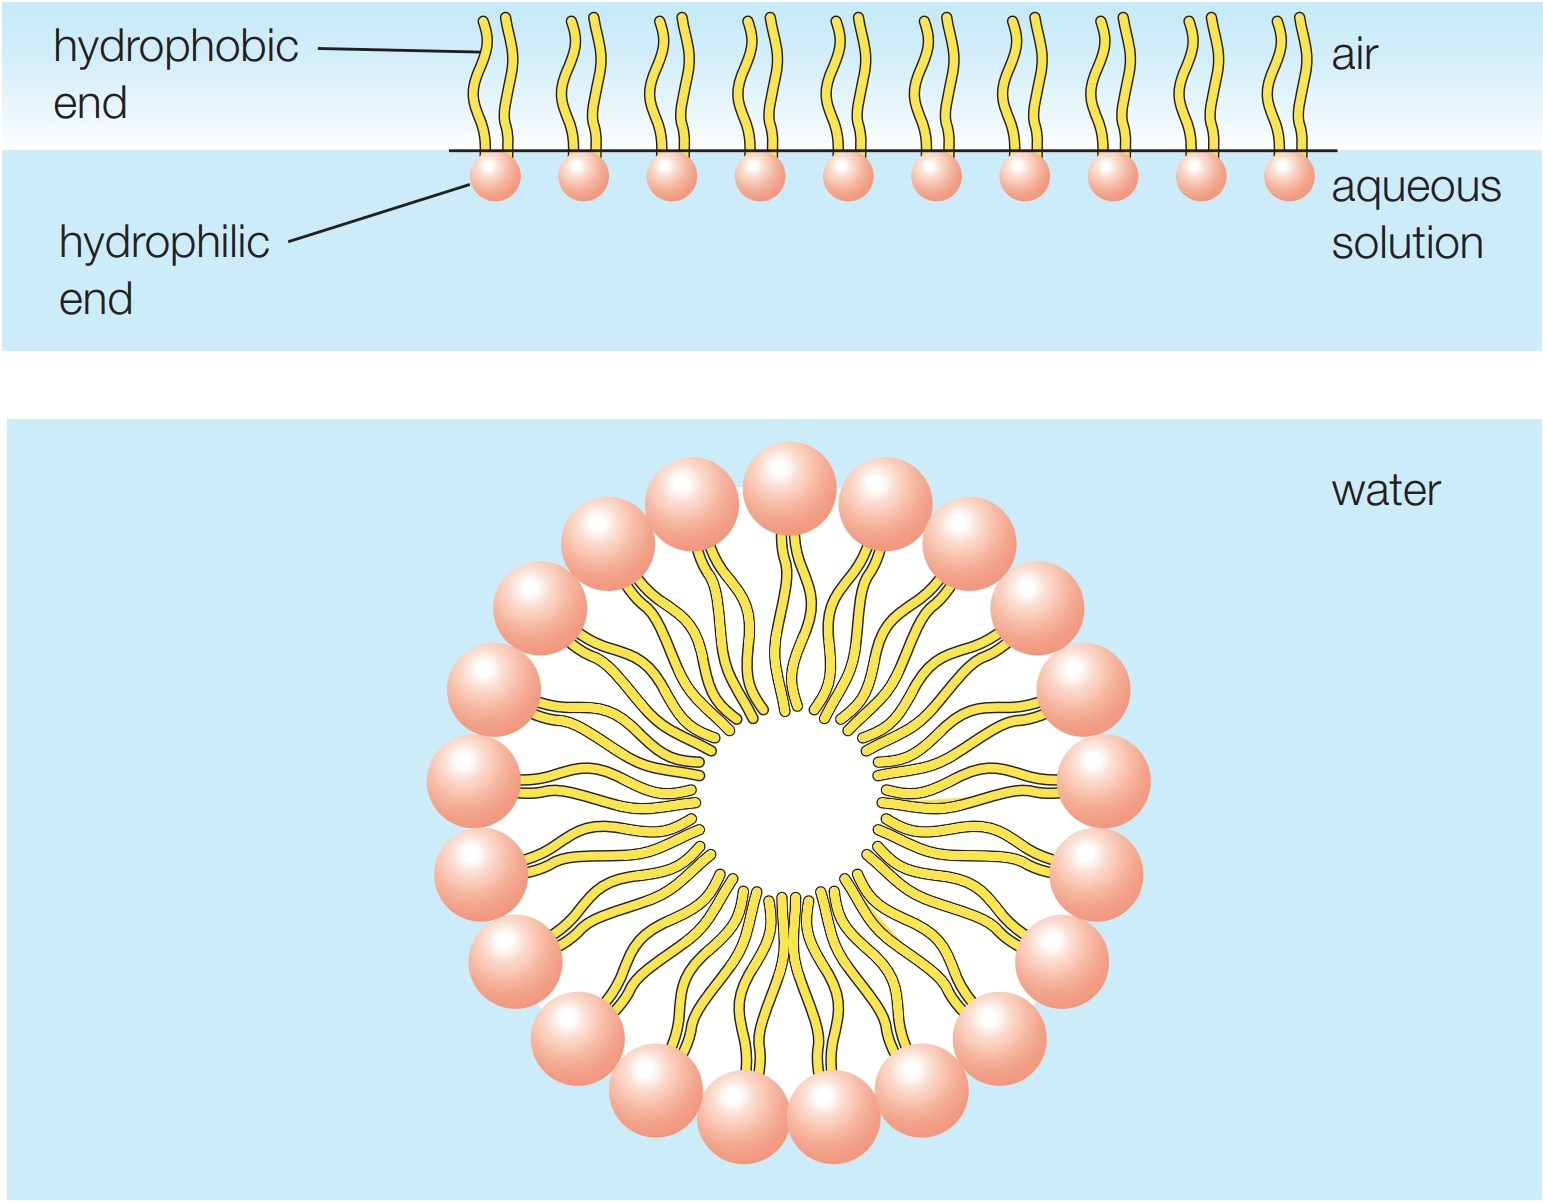
\includegraphics[scale=0.12]{Biology/2A/Images/2A-1-2.png}
            \caption{Phospholipids form a monolayer at an air / water junction and a micelle when water surrounds them.}
        \end{figure}
    \end{itemize}
    \item \textbf{Properties of the Bilayer}
    \begin{itemize}
        \item Acts as a barrier to most molecules.
        \item Allows fat-soluble molecules to pass but not ions.
        \item More fluid with unsaturated fatty acids.
        \item Cholestrol makes the membrane stronger and less \underline{permeable} (渗透性).
    \end{itemize}
\end{itemize}

\paragraph{\underline{The Fluid Mosaic Model} (流动镶嵌模型)}
\begin{itemize}
    \item Proposed by S. J. Singer and G. Nicolson in 1972.
    \item Membrane is dynamic, not rigid.
    \item Proteins float inthe lipid bilayer.
    \begin{itemize}
        \item \underline{Integral proteins} (整合蛋白) span the membrane.
        \item \underline{Peripheral proteins} (外周蛋白) are attached to the surface.
        \item \underline{Glycoproteins} (糖蛋白) help in cell recognition.
    \end{itemize}
    \begin{figure}[H]
        \centering
        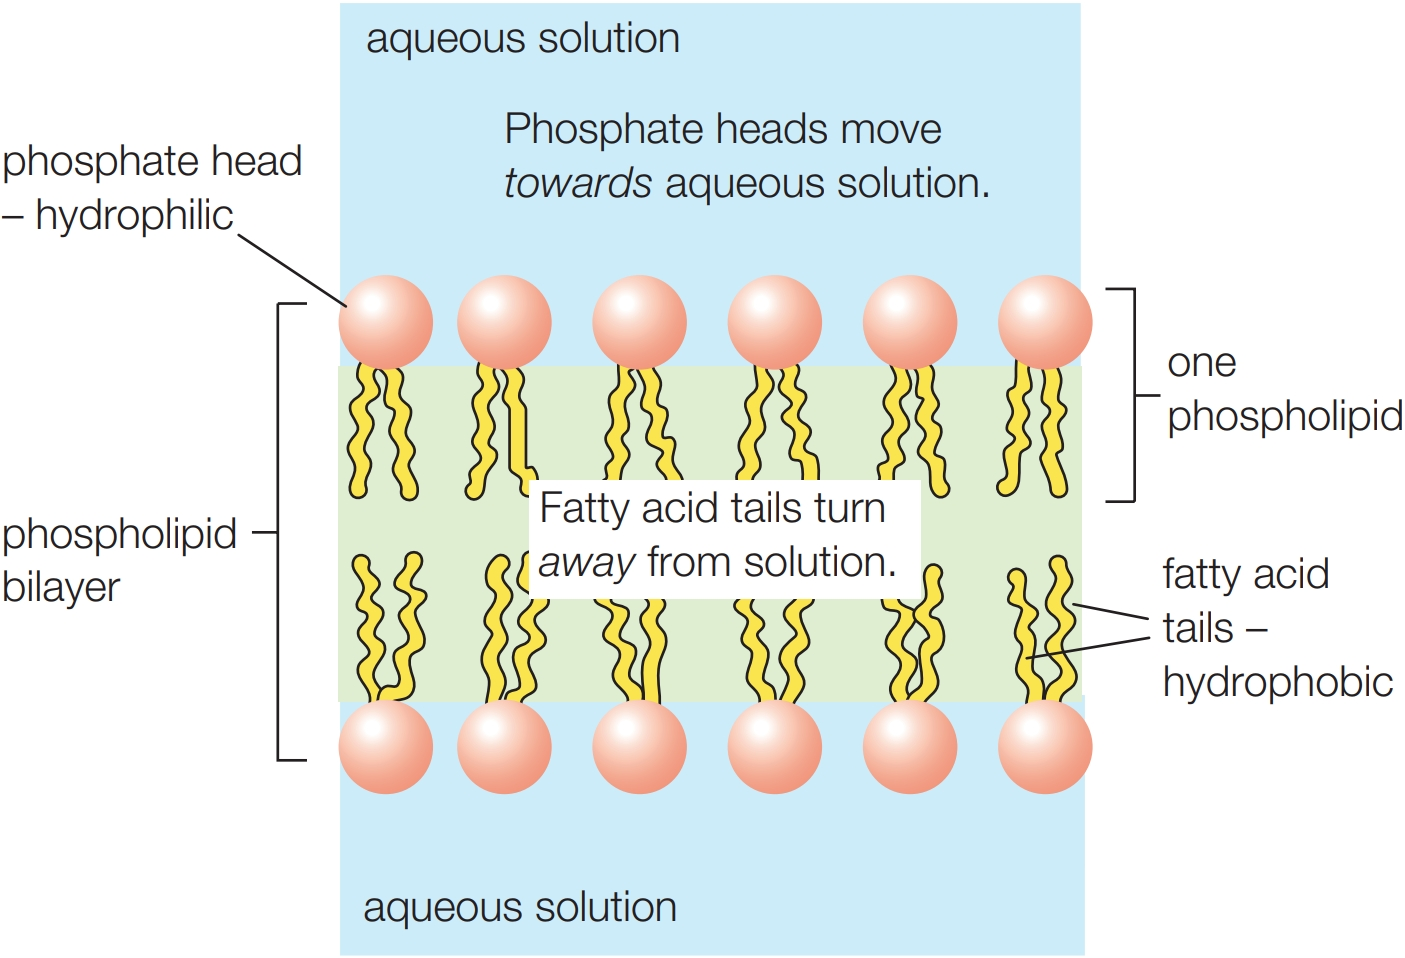
\includegraphics[scale=0.15]{Biology/2A/Images/2A-1-3.png}
        \caption{Phospholipids form a monolayer at an air / water junction and a micelle when water surrounds them.}
    \end{figure}
    \item \textbf{Functions of Membrane Proteins}
    \begin{itemize}
        \item \textbf{Transport:} Gated channels allow specific molecules through.
        \item \textbf{\underline{Receptors} (受体):} Detect hormones / signals.
        \item \textbf{Enzymes:} Speed up reactions.
        \item \textbf{Glycoproteins:} Involved in cell recognition.
    \end{itemize}
\end{itemize}

\paragraph{Scientific Models of Membranes}
\begin{itemize}
    \item Early experiments showed membranes contained lipids.
    \item 1935: \underline{Davson-Danielli Model} (达夫森-丹尼利模型) - Membrane had a lipid core with a protein layer.
    \item 1950s: \underline{Electron Microscopy} (电子显微镜) confirmed a bilayer.
    \item 1972: \underline{Fluid Mosaic Model} (流动镶嵌模型) replaced older models after further studies.
    \begin{figure}[H]
        \centering
        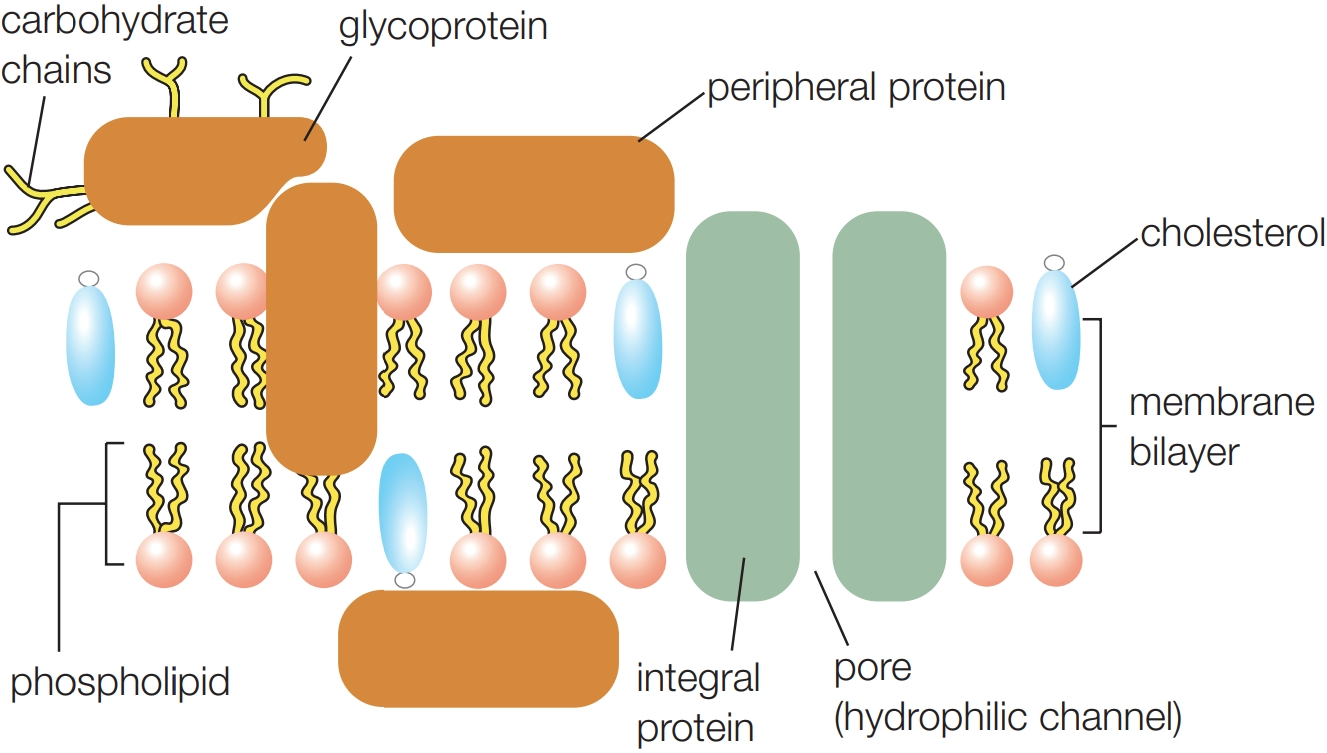
\includegraphics[scale=0.18]{Biology/2A/Images/2A-1-4.png}
        \caption{The fluid mosaic model of the cell membrane - a phospholipid sea with associated proteins, which may be floating
        or anchored within the membrane.}
    \end{figure}
\end{itemize}

\paragraph{Investigating Membrane Properties}
\begin{itemize}
    \item \underline{Red beet experiments} (红甜菜实验): More red \underline{dye} (染料) in water = more permeable membrane.
    \item Alcohol dissolves lipids, increasing permeability.
    \item High temperature \underline{denatures} (变性) proteins, making membranes leaky.
\end{itemize}

\paragraph{Exam Keys}
\begin{itemize}
    \item Phospholipid bilayer = barrier, but proteins control permeability.
    \item Membranes are flexible and fluid, not rigid.
    \item Cholesterol increases strength and reduces permeability.
    \item Use experimental data to explain membrane permeability changes.
\end{itemize}
% ===============================
%          Chapter 2A.2
%  Cell Transport and Diffusion
%     Created by Michael Tang
%           2025.02.16
% ===============================

\subsubsection{2A.2 Cell Transport and Diffusion}
\paragraph{Types of membrane transport}
Substance move across membranes via passive transport (no energy required / no ATP used) or active transport (energy required /
ATP used).
\begin{itemize}
    \item \textbf{Diffusion:} No energy required / no ATP used. Molecules move from high concentration to low concentration.
    Random movement of molecules.
    \item \textbf{Facilitated diffusion:} No energy required / no ATP used. Molecules move from high concentration to low
    concentration. Uses carrier or \underline{channel proteins} (管道蛋白).
    \item \textbf{Osmosis:} No energy required / no ATP used. Movement of water molecules from high concentration to low
    concentration. Water moves through a selectively \underline{permeable membrane} (渗透膜).
    \item \textbf{Active transport:} Energy required / ATP used. Molecules move from low concentration to high concentration.
    Uses carrier proteins.
    \item \textbf{\underline{Endocytosis} (内吞作用):} Energy required / ATP used. Molecules move into the cell.
    \underline{Vesicle} (囊泡) forms around the substance.
    \item \textbf{\underline{Exocytosis} (胞吐作用):} Energy required / ATP used. Molecules move out of the cell.
    Vesicle fuses with the cell membrane.
\end{itemize}

\paragraph{Passive Diffusion}
No ATP required - molecules move down a concentration gradient.
\begin{itemize}
    \item \textbf{Diffusion}
    \begin{itemize}
        \item Movement of molecules from high concentration to low concentration due to \underline{kinetic energy} (动能).
        \item Example: Oxygen (\ce{O2}) and carbon dioxide (\ce{CO2}) diffuse freely across the cell membrane.
    \end{itemize}
    \begin{figure}[H]
        \centering
        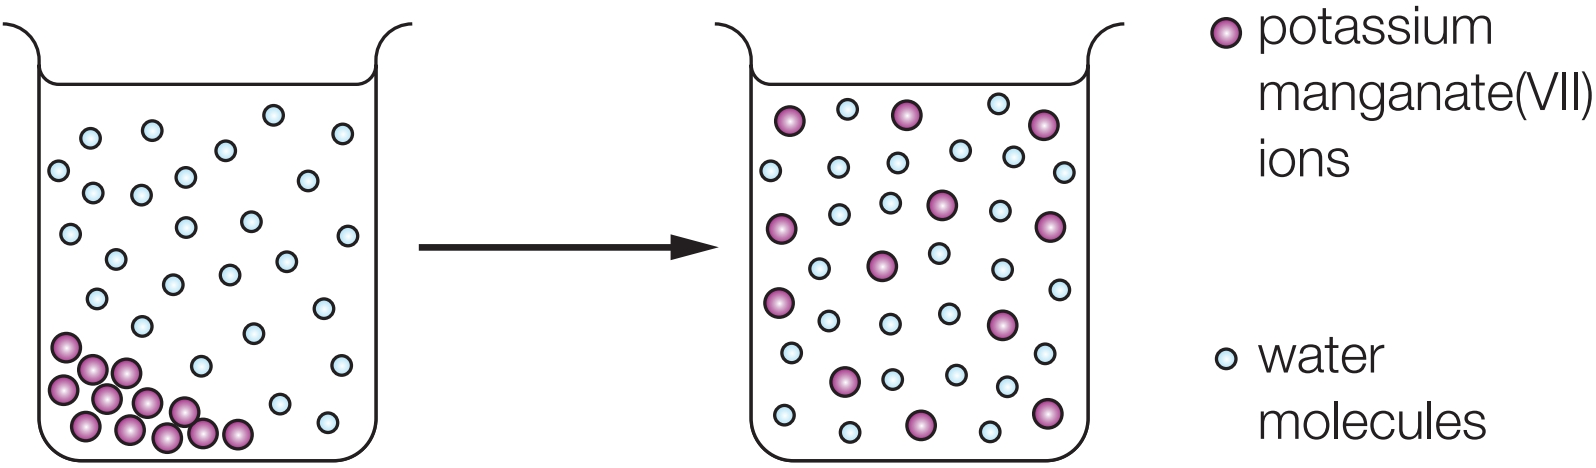
\includegraphics[scale=0.12]{Biology/2A/Images/2A-2-1.png}
        \caption{If the beaker is left to stand, diffusion takes place as the random movement of both the water and the
        \underline{potassium manganate (VII) ions} (\ce{MnO4^-}) ensures that they become evenly mixed.} 
    \end{figure}
    \item \textbf{Facilitate Diffusion}
    \begin{itemize}
        \item \textbf{Larger / polar molecules} (e.g., glucose, amino acids) need carrier or channel proteins.
        \item \textbf{Channel proteins}
        \begin{itemize}
            \item Specific to certain ions / molecules.
            \item Can be gated (open / close in response to signals).
        \end{itemize}
        \textbf{Carrier proteins:} Bind to a molecule and change shape to move it across the membrane.
    \end{itemize}
    \begin{figure}[H]
        \centering
        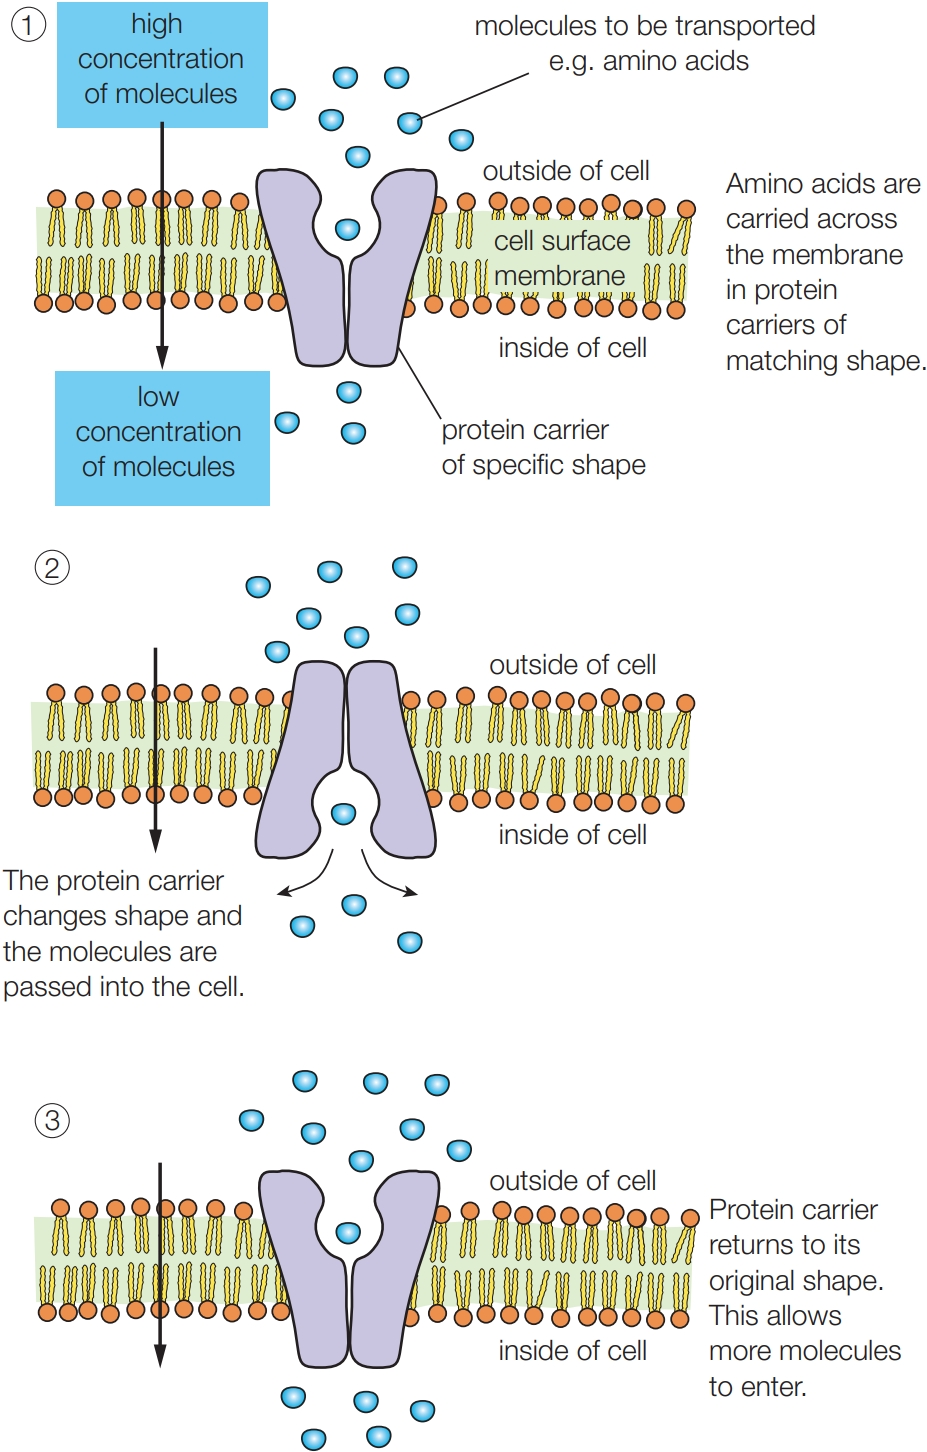
\includegraphics[scale=0.25]{Biology/2A/Images/2A-2-2.png}
        \caption{Facilitated diffusion acts as a ferry across the lipid membrane sea. It is not an active process, so it can only
        work when the concentration gradient is in the right direction.} 
    \end{figure}
    \item \textbf{Osmosis}
    \begin{itemize}
        \item The movement of water molecules from a high water potential to a low water potential.
        \item Occurs through a partially permeable membrane.
    \end{itemize}
\end{itemize}

\paragraph{Active Transport (ATP Required)}
\begin{itemize}
    \item Moves molecules against the concentration gradient.
    \begin{itemize}
        \item Uses carrier proteins powered by ATP.
        \item Example: \underline{Sodium-potassium pump} \footnote{The sodium-potassium pump (\ce{Na^+} / \ce{K^+} pump) is a
        type of active transport that moves sodium (\ce{Na^+}) out of the cell and potassium (\ce{K^+}) into the cell, against
        their concentration gradients. This process requires ATP and helps maintain the resting membrane potential in nerve and
        muscle cells. The pump exchanges 3\ce{Na^+} ions out for 2\ce{K^+} ions in, making the inside of the cell more negative
        compared to the outside. This is essential for nerve impulse transmission, muscle contraction, and overall cell function.}
        (钾钠泵) in nerve cells.
    \end{itemize}
    \item \textbf{\underline{Endocytosis} (内吞作用) and \underline{Exocytosis} (胞吐作用)}
    \begin{itemize}
        \item \textbf{Endocytosis:} Large molecules enter the cell by forming vesicles.
        \item \textbf{Exocytosis:} Large molecules exit the cell by \underline{vesicle fusion} \footnote{Vesicle fusion is the
        process by which a vesicle, a small \underline{membrane-bound sac} (膜结合囊 / 膜包囊) containing substances, fuses with
        the cell membrane to release its contents into or out of the cell. This is a key mechanism in exocytosis (moving
        substances out of the cell) and endocytosis (bringing substances into the cell). During fusion, the vesicle membrane
        merges with the cell membrane, allowing the vesicle's contents, such as hormones or waste products, to be transported
        across the membrane. This process often requires energy in the form of ATP.} (囊泡融合) with the membrane.
        \item Example: Secretion of enzymes, hormones, \underline{neurotransmitters} \footnote{Neurotransmitters are chemical
        messagers that transmit signals across a \underline{synapse} (突触, the gap between two nerve cells). They are released
        from the \underline{axon terminal} (轴突终末) of a neuron and bind to \underline{receptors} (受体 / 感受器) on the
        \underline{dendrites} (树突) of the next neuron triggering a response. Neurotransmitters play a key role in nerve signals
        transmission, influencing functions like mood, movement, and \underline{cognition} (认知). Examples include
        \underline{dopamine} (多巴胺, related to reward and movement), \underline{serotonin} (血清素 / 五羟色胺, influences mood
        and sleep), and \underline{acetylcholine} (乙酰胆碱, involved in muscle contraction). The proper balance of
        neurotransmitters is essential for normal brain function} (神经递质).
    \end{itemize}
\end{itemize}

\paragraph{Exam Keys}
\begin{itemize}
    \item Diffusion = kinetic energy only, no ATP.
    \item Facilitated diffusion uses proteins but still no ATP.
    \item Active transport uses ATP and carrier proteins to move substances against a gradient.
    \item Endocytosis and exocytosis uses vesicles for bulk transport.
\end{itemize}
% ======================================
%            Chapter 2A.3
%  Osmosis: A Special Case of Diffusion
%        Created by Michael Tang
%             2025.02.17
% ======================================

\subsubsection{2A.3 Osmosis: A Special Case of Diffusion}
\paragraph{What is Osmosis?}
\begin{itemize}
    \item Osmosis is the movement of free water molecules through a partially permeable membrane from an area of high water
    potential to an area of low water potential.
    \item Water potential is a measure of the potential for water to move in or out of a solution due to osmosis. It depends on
    the concentration of free water molecules.
    \item Water always moves doen the water potential gradient, meaning form areas of high water potential (more free water
    molecules) to low water potential (less free water molecules).
    \item Water moves through membranes, but solute molecules cannot move in the same way.
    \begin{figure}[H]
        \centering
        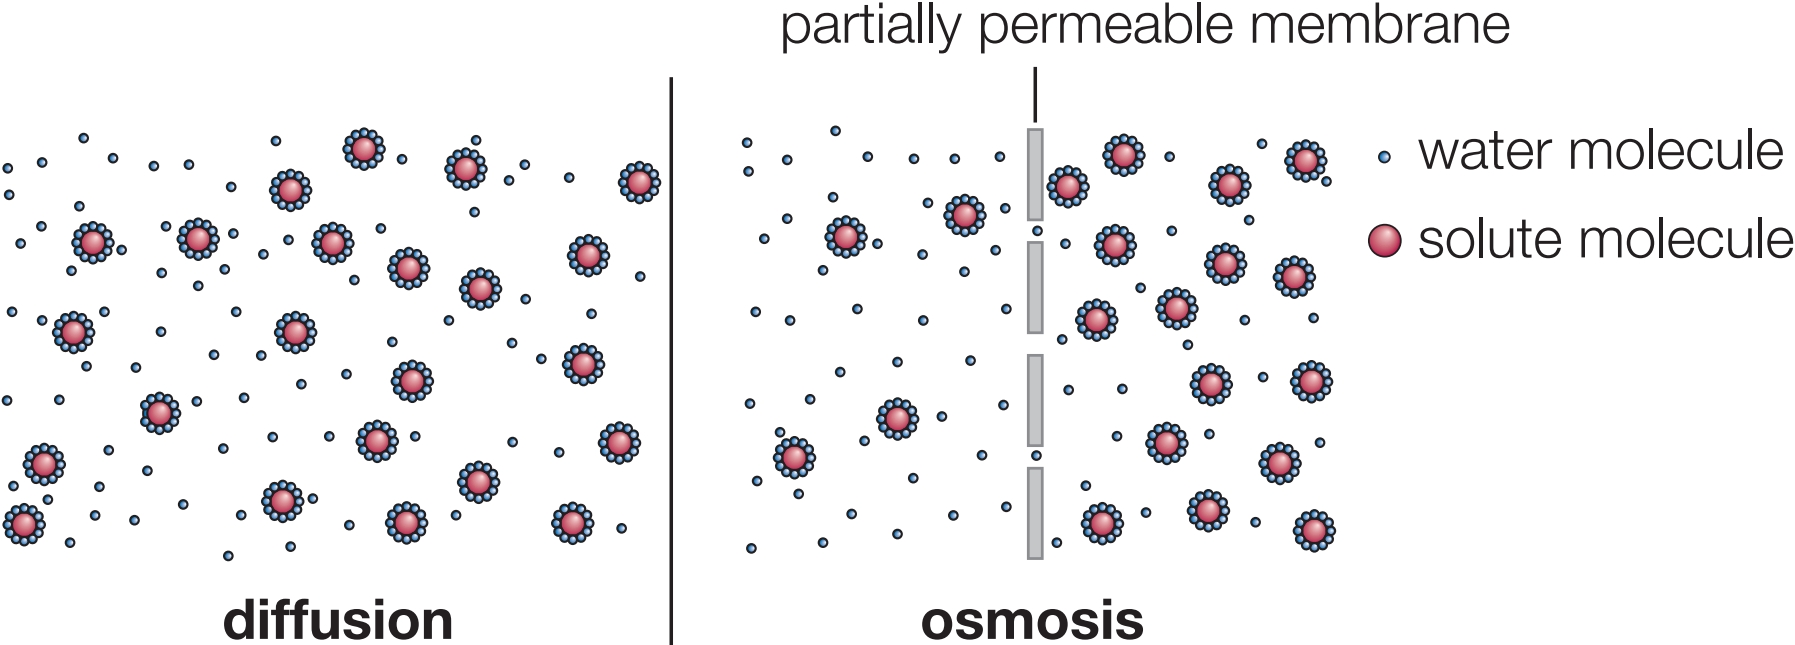
\includegraphics[scale=0.12]{Biology/2A/Images/2A-3-1.png}
        \caption{In diffusion, the random movement of particles results in an even distribution of both solute and solvent
        particles. In osmosis, a partially permeable membrane means only solvent molecules and very small solute particles can
        move freely.}
    \end{figure}
\end{itemize}

\paragraph{Osmotic Concentrations}
\begin{itemize}
    \item Osmotic concentration refers to the amount of dissolved solutes in a solution. A solution with more solutes has lower
    water potential.
    \item Solutions are categorized as:
    \begin{itemize}
        \item \textbf{\underline{Isotonic solution} (等渗溶液):} The concentration of solutes is the same as inside the cell.
        \item \textbf{\underline{Hypotonic solution} (低渗溶液):} The concentration of solutes is lower than inside the cell,
        causing water to enter the cell.
        \item \textbf{\underline{Hyperonic solution} (高渗溶液):} The concentration of solutes is higher than inside the cell,
        causing water to leave the cell.
    \end{itemize}
\end{itemize}

\paragraph{Osmosis in Animal Cells}
Animal cells must maintain a delicate balance of water to prevent cell bursting or shrinking.
\begin{itemize}
    \item \textbf{Hypotonic solution:} Water enters the cell, causing it to swell and burst.
    \item \textbf{Hypertonc solution:} Water leaves the cell, causing it to shrink and shrivel.
\end{itemize}
\begin{figure}[H]
    \centering
    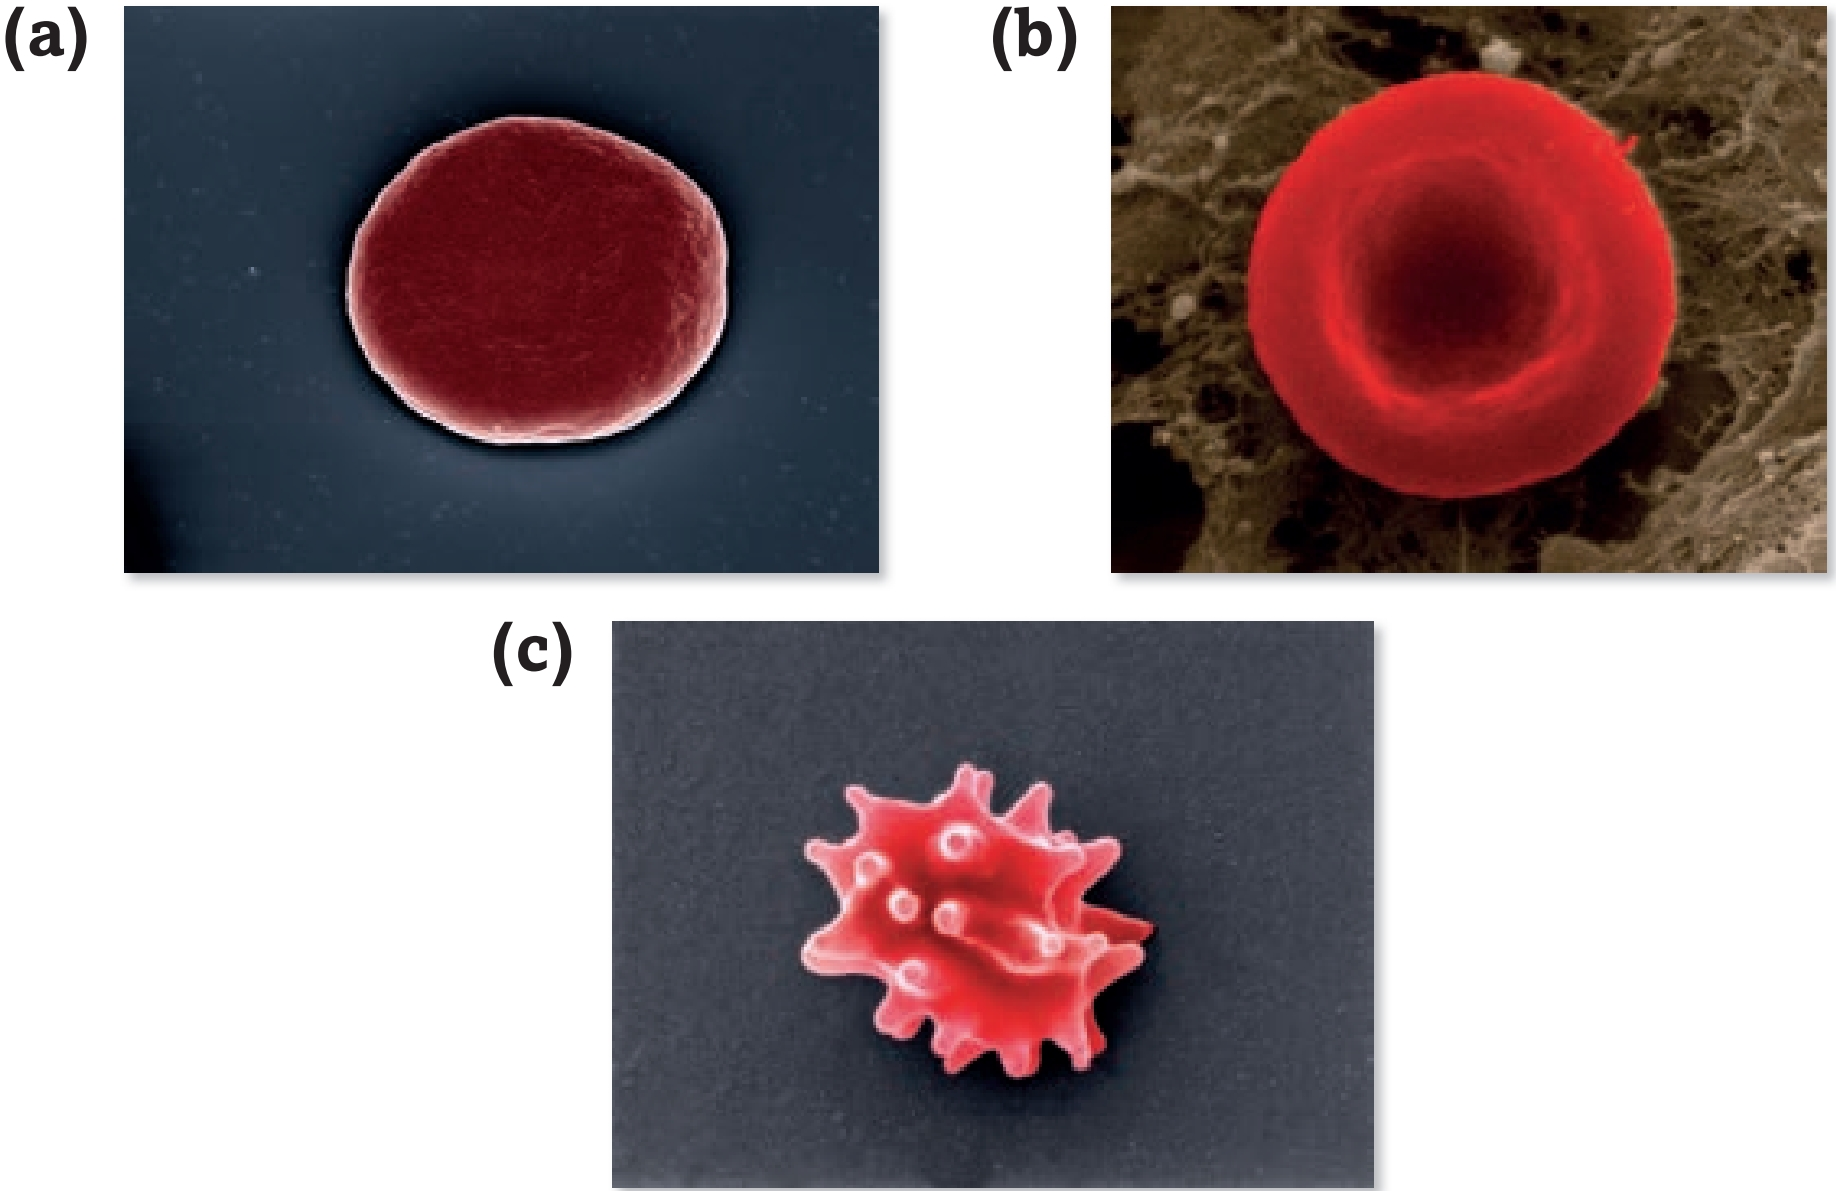
\includegraphics[scale=0.12]{Biology/2A/Images/2A-3-2.png}
    \caption{The effects of osmosis on red blood cells show why the systmes of the body that maintain solute concentrations and
    water balance are so important. \textbf{(a)} In hypotonic solution, water moves in and the cell swells and brusts;
    \textbf{(b)} in isotonic solution the red blood cell maintains its normal shape; \textbf{(c)} in hypertonic solution, water
    moves out and the cell shrinks.}
\end{figure}

\paragraph{Osmosis in Plant Cells}
Plant cells are more resistant to osmotic pressure due to their rigid cell walls.
\begin{itemize}
    \item \textbf{Hypotonic solution:} Water enters the cell, causing it to swell and generate hydrostatic pressure (inward
    pressure that prevents further water influx). This is called \underline{turgor} (膨压).
    \item \textbf{Hypertonic solution:} Water exits the cell, causing the \underline{protoplast} (原生质, cell contents) to
    shrink from the cell wall in a process called \underline{plasmolysis} (胞质裂解).
\end{itemize}
\begin{figure}[H]
    \centering
    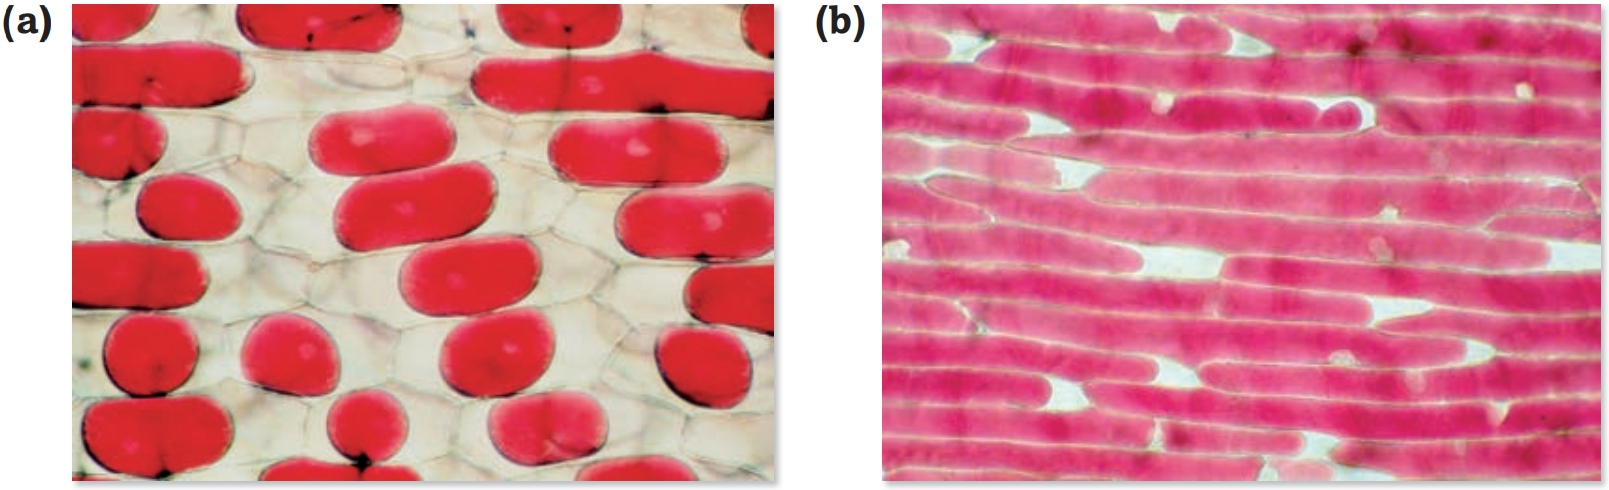
\includegraphics[scale=0.15]{Biology/2A/Images/2A-3-3.png}
    \caption{Plant cells from red beet showing \textbf{(a)} plasmolysis; and \textbf{(b)} turgor.}
\end{figure}

\paragraph{Modelling Osmosis in Cells}
\begin{itemize}
    \item \textbf{Experimental model:} We can model osmosis using an artificial membrane to \underline{demonstrate} (证明) the
    movement of water through a \underline{partially permeable membrane} (半透膜).
    \item \textbf{Sucrose solution} can be used to \underline{illustrate} (说明) osmotic movement (water moves to the area with
    higher solute concentration).
\end{itemize}

\paragraph{Exam Tips}
\begin{itemize}
    \item Use the term water potential to explain osmotic movement in and out of cells.
    \item \textbf{Remember the gradient:} Water always moves from high to low water potential.
    \item Osmosis requires \textbf{no ATP} - It is a passive process relying on kinetic energy of water molecules.
\end{itemize}

\chapter{Chemistry}

\section{Formulae, Equations and Atoms of Substances}

\subsection{Atoms, Elements and Molecules}
% ===============================================
%                 Chapter 1A.1
%  Techniques for Measuring the Rate of Reaction
%             Created by Michael Tang
%                  2024.12.30
% ===============================================

\subsubsection{1A.1 Techniques for Measuring the Rate of Reaction}
\paragraph{What is an Element?}
\begin{itemize}
    \item \textbf{Definition of an Element:} A pure substance that cannot be broken down into simpler substances through
    chemical reactions.
    \begin{itemize}
        \item It consists of only one type of atom.
        \item Represented on the \underline{Periodic Table} (元素周期表) by a one or two-letter symbol. Example: \ce{H} for
        hydrogen, \ce{Ne} for neon.
    \end{itemize}
    \item \textbf{Periodic Table Representation}
    
\end{itemize}


\chapter{Physics}


% Bibliography
%\chapter*{Bibliography}
%\addcontentsline{toc}{chapter}{Bibliography}
%\begin{thebibliography}{9}
%\bibitem{author1} Author Name. \textit{Book Title}. Publisher, Year.
%\bibitem{author2} Author Name. \textit{Book Title}. Publisher, Year.
%\end{thebibliography}

\end{document}
